\documentclass[11pt]{article}
\usepackage[margin=1in]{geometry}
\usepackage{amsmath,amssymb,amsthm,mathtools}
\usepackage{booktabs}
\usepackage[colorlinks=true,linkcolor=blue!50!black,citecolor=blue!50!black,urlcolor=blue!50!black]{hyperref}
\usepackage{xcolor}
\usepackage{graphicx}

\newtheorem{theorem}{Theorem}
\newtheorem{proposition}[theorem]{Proposition}
\newtheorem{lemma}[theorem]{Lemma}
\newtheorem{corollary}[theorem]{Corollary}
\theoremstyle{definition}
\newtheorem{definition}[theorem]{Definition}
\newtheorem{remark}[theorem]{Remark}
\newtheorem{problem}[theorem]{Open problem}

\newcommand{\E}{\mathbb{E}}
\newcommand{\Var}{\operatorname{Var}}
\newcommand{\Aut}{\operatorname{Aut}}
\newcommand{\Unif}{\operatorname{Unif}}
\newcommand{\norm}[1]{\lVert #1\rVert}
\newcommand{\cH}{\mathcal H}
\newcommand{\hgt}{\operatorname{ht}}
\newcommand{\R}{\mathbb R}
\newcommand{\Cov}{\operatorname{Cov}}

\title{Learning a Self-Similar Grammar from One Example:\\
Tied Random Hierarchy Models, Context Clustering, and the Value of Scale Symmetry}
\author{Companion note to ``Self-Similar Recursive Grids'' (srg.pdf), Open Problem 9.2}
\date{September 2026}

\begin{document}
\maketitle

\begin{abstract}
The Random Hierarchy Model (RHM) is a synthetic compositional task: a context-free grammar of
depth $L$ with $v$ symbols, $m$ synonymous rules per symbol, and branching $s$. Backprop-trained
deep CNNs need $P^*\propto v\,m^L$ labelled examples \cite{cagnetta2024}. Latent-prediction
methods need $\asymp v m^3$ examples, which is independent of $L$ \cite{korchinski2026}. In both
lines of work the rules are drawn \emph{independently at every level}. We study the
\emph{tied} (self-similar) RHM, in which one grammar is used at every level. This is the
stochastic-process counterpart of the scale-tied recursive grid. Three results follow.
\textbf{(1) Without tying, labels are unavoidable.} In the untied RHM, \emph{every} learner has
root accuracy at most $1/v+P/(vm)$ from $P$ labelled examples. This holds even with unlimited
unlabelled data and an oracle for all lower-level rules, because the top rule has no context.
\textbf{(2) With tying, clustering bottom tuples by their sibling context recovers the grammar.}
This rule is a statistical form of the Myhill--Nerode quotient. Given the latents at height
$\ge2$, the $s^{L-2}$ bottom grids of each example are independent, so correlations inside a
tree enter only through one non-degeneracy condition. The number of examples needed falls like
$s^{-(L-2)}$. \textbf{(3) The clusters are named by self-similarity.} The consistent namings are
exactly a coset of the automorphism group of the valid-tuple set, which is trivial with high
probability. Together: from a \emph{single unlabelled example} of sufficient depth, the learner
recovers the grammar exactly and classifies the root perfectly, without labels or backpropagation.
Experiments ($v{=}8$, $m{=}4$, $s{=}2$) confirm this. Exact recovery needs about $1024$--$2048$ bottom
grids however they are packaged into trees, and one example suffices from $L=11$ on. Backprop through
untied or tied CNNs with root labels moves the other way: its label requirement roughly doubles
per level ($512$ at $L=2$, $16384$ at $L=6$), and the tied architecture alone does not help it.
The gap between backprop's labelled examples and the context learner's unlabelled examples is
therefore $1\times$ at $L=2$ and $512\times$ at $L=6$.
\textbf{(4) Partial tying degrades gracefully.} If each rule at each level is reused with
probability $\rho$ and replaced otherwise, every zero-label learner has error at least
$\approx(1-\rho)(1-1/v)$, the root's own unexplained rules. A level-wise learner attains this
floor up to an $O((1-\rho)vm\log(vmL)/P)$ term, and \emph{neither bound depends on depth}: the
number of nodes at a level controls both how easily its deviations are learned and how often they
matter, and the two effects cancel. Experiments reach the floor at every depth for
$0.6\le\rho\le0.9$, and the breakdown near $\rho=0.5$ is explained.
\textbf{(5) The gains are not an artifact of discreteness.} In a linear-Gaussian self-similar
tree, the same pipeline carries over: sibling moments whose within-tree correlations cancel, and
naming as fixing the latent basis by self-similarity (unique up to the Gaussian sign symmetry).
It learns from one unlabelled tree of depth 9, while an untied tree provably needs labels. What
does \emph{not} carry over is backprop's exponential label cost, which is a combinatorial effect:
in the linear model backprop needs a few hundred labels at any depth tested.
\textbf{(6) The mechanism is general.} For an arbitrary tied tree process (noisy, continuous,
nonlinear), context identifies each grid's belief about its parent, i.e.\ its belief-propagation
message; estimating it depends on the data only through the total number of bottom grids; and
naming is identified up to the automorphisms of the kernel, which additive Gaussian noise reduces
to a finite-dimensional group of isometries commuting with the sibling maps. For bounded nonlinear
Gaussian trees, the laws of the bottom two levels (hence one deep tree) determine the noise, the
kernel and its naming up to that group, with no labels (\S\ref{sec:general}, Theorem~\ref{thm:ngt}).
\textbf{(7) Why backprop slows with depth.} The correlation between the root label and any local
feature of the leaves decays like $q_1^{L/2}$, where $q_1\le s\lambda^2$ is a linear Kesten--Stigum
number of the kernel. The first phase of gradient descent sees only this signal. Gaussian trees have
no gap (their Bayes predictor is linear); tied grammars with $q_1<1$ do. For the grammars above
$q_1\approx0.4$, and $1/q_1$ matches the measured growth of backprop's labels per level
(\S\ref{sec:claim2}).
\textbf{(8) Real images.} On CIFAR-10 the state of a region is its $2\times2$ thumbnail, which is
parent-determined and observed, together with a hidden context type that context theory requires
(siblings stay dependent given the thumbnail). Sum--product over types is then exact, and the tree is an
exact density on images. With zero labels it reaches $4.75$ bits/dim, and its samples reproduce the
per-scale heavy tails of natural images. Its excess loss from $N$ unlabelled images is $\approx2.5k/(2N)$
spread over all scales, while an untied top pays the predicted $492/N$ bits per coordinate. About $10^3$
images give the kernel that $5\cdot10^4$ give. A linear head on the root is the Bayes readout, but a
likelihood-trained root holds little class information ($0.30$--$0.38$). The top scale is where CIFAR
stops being self-similar (\S\ref{sec:cifar}). The class information is not lost in the tree but at its
last merge: the four quadrant states give $0.55$, and the hidden types add to the thumbnails at every scale.
Observing labels at the root in the joint likelihood costs at most $H(Y)$ per image in density, and it can
therefore move only what the pixels leave undecided. The root type is already decided by the pixels, so labels add
little ($0.17\to0.25$ with an untied top). An observed label's influence on a node falls about twentyfold per
level on CIFAR, and it bounds the root-label backprop gradient there as well (\S\ref{sec:semtop}).
\end{abstract}

%==========================================================================
\section{Models}
%==========================================================================
Let $V=\{1,\dots,v\}$ and fix a branching $s\ge2$. A \emph{grammar} $G=(R_a)_{a\in V}$ assigns to
each symbol $m$ rules $R_a\subset V^s$, $|R_a|=m$, and the sets are pairwise disjoint
(unambiguity). Write $D=\bigcup_aR_a$ ($|D|=vm$) for the valid tuples,
$f=m/v^{s-1}\in(0,1]$ for their fraction, and $g:D\to V$ for the parent map. For the random
grammar, $D$ is a uniformly random $vm$-subset of $V^s$, partitioned uniformly into $v$ blocks
of size $m$.

\begin{definition}[tied and untied RHM]
Draw the root $z_\epsilon\sim\Unif(V)$. Every internal node $w$ independently picks a rule
uniformly from $R^{(\hgt(w))}_{z_w}$, and its $s$ children take the symbols of that rule. The
input is the $s^L$ leaf symbols and the label is $y=z_\epsilon$. In the \emph{untied} RHM of
\cite{cagnetta2024,korchinski2026}, $R^{(h)}$ are independent random grammars. In the
\emph{tied} RHM (SRHM), $R^{(h)}=R$ at every height.
\end{definition}

For both models, knowing the grammar(s) makes classification trivial: parse bottom-up with
$g$. For the tied model this is a discrete scale-tied recursive grid with state space
$V\cup\{\bot\}$ and one table $g$ (srg.pdf, \S3). By the Myhill--Nerode theorem for grids, the
minimal grid for the task has exactly the grammar's symbols as states. \emph{Learning the
grammar means finding the synonym partition of $D$ and naming its blocks.}

%==========================================================================
\section{Without tying, labels are unavoidable}
%==========================================================================
\begin{theorem}\label{thm:lower}
In the untied RHM with a uniformly random top grammar $R^{(L)}$, consider any learner that
receives $P$ labelled examples, any number of unlabelled examples, and the lower-level grammars
$R^{(1)},\dots,R^{(L-1)}$ exactly. Its expected root accuracy on a fresh example is at most
\[
\frac1v+\frac{P}{vm}.
\]
Accuracy $1-\varepsilon$ therefore needs $P\ge(1-\tfrac1v-\varepsilon)\,vm$ labels.
\end{theorem}
\begin{proof}
Given the lower grammars, the leaves determine the top tuple $u\in D_L$ (the root's children),
and nothing more is relevant. For every example, $u$ is uniform on $D_L$. Conditioned on $u$
and the root, the rest of the tree does not depend on how $D_L$ is partitioned. Unlabelled data
therefore reveal at most $D_L$. By exchangeability of the random partition, the posterior given
$D_L$ and the $U\le P$ distinct labelled top tuples is uniform over the partitions consistent
with them. A test tuple $u^*$ is one of the labelled tuples with probability $U/(vm)$. Otherwise
its parent is $a$ with probability $(m-k_a)/(vm-U)\le m/(vm-U)$, where $k_a$ counts the labelled
tuples with parent $a$. The success probability is at most
$\frac{U}{vm}+\big(1-\frac{U}{vm}\big)\frac{m}{vm-U}=\frac{U}{vm}+\frac1v$.
\end{proof}
\noindent The top grid is the one grid without context. Nothing below it can reveal which
tuples are synonyms at the top, and only labels can. Latent-prediction learners
\cite{korchinski2026} recover levels $1,\dots,L-1$ without labels, but the last level still
costs $\Theta(vm)$ labels. \emph{Tying removes this barrier.} The top level uses the same
partition as the bottom level, where every tuple has abundant context.

%==========================================================================
\section{With tying: context clustering at the bottom}
%==========================================================================
Let $\cH_2$ be the latents at all heights $\ge2$, and let $b_w$ be the symbol of a height-2 node
$w$ (a \emph{grid} whose $s$ children are bottom tuples). Let $n_b$ be the number of grids with
$b_w=b$, pooled over the $P$ examples, and $n_2=\sum_bn_b=Ps^{L-2}$. For $b\in V$ and ordered
positions $i\ne j$, let $c_b(a,a')=\#\{r\in R_b:(r_i,r_j)=(a,a')\}$ and
$c_b(a)=\sum_{a'}c_b(a,a')$. Given a histogram $n=(n_b)$, the \emph{realized sibling law} is
\[
\nu^{n}(a'\mid a)=\frac{\sum_bn_b\,c_b(a,a')}{\sum_bn_b\,c_b(a)},\qquad
\Delta(n)=\min_{a_1\ne a_2}\norm{\nu^n(\cdot\mid a_1)-\nu^n(\cdot\mid a_2)}_1 .
\]
For a bottom tuple $t$, let $\hat\mu_t$ be the empirical distribution of the tuple at position $j$
over all grids having $t$ at position $i$.

\begin{lemma}[statistical Myhill--Nerode]\label{lem:ctx}
Conditioned on $\cH_2$, the grids are independent. For $t\in R_a$, the conditional mean of
$\hat\mu_t$, reweighted by selection probabilities, is
\[
\mu^n_t=\sum_{a'}\nu^n(a'\mid a)\,\Unif(R_{a'}),
\]
which depends on $t$ \emph{only through its parent $a$}. Synonymous tuples have identical context
laws, and tuples with parents $a_1\ne a_2$ have context laws at $L^1$ distance
$\norm{\nu^n(\cdot|a_1)-\nu^n(\cdot|a_2)}_1\ge\Delta(n)$.
\end{lemma}
\begin{proof}
Given $\cH_2$, grid $w$ picks $r\sim\Unif(R_{b_w})$, and its children pick $t_{wk}\sim\Unif(R_{r_k})$
independently. So $P(t_{wi}=t,t_{wj}=t')=c_{b_w}(a,a')/m^3$ for $t\in R_a$, $t'\in R_{a'}$.
Summing over grids and normalizing gives $\mu^n_t$. The $L^1$ identity holds because the
$\Unif(R_{a'})$ have disjoint supports.
\end{proof}
\noindent This is the context-equivalence of srg.pdf, Thm.~3.2, in statistical form. Two grids
are merged when \emph{no context distinguishes them}, and here the context is the sibling. It is
also the ``copy grids with equal histories'' rule of the original notes.

\begin{theorem}[partition recovery; correlation-free]\label{thm:rec}
Condition on $\cH_2$ with $\Delta(n)\ge\Delta_0>0$. Let $\gamma_a=\sum_bn_bc_b(a)/(m\,n_2)$ be the
realized frequency of parent $a$ at position $i$, and $\gamma_{\min}=\min_a\gamma_a$. There is
an absolute constant $C$ such that, if
\[
n_2=P\,s^{L-2}\ \ge\ C\,\frac{v\,m^2\log(vm/\delta)}{\Delta_0^2\,\gamma_{\min}},
\]
then with probability $\ge1-\delta$ every $t\in D$ satisfies
$\norm{\hat\mu_t-\mu^n_t}_1\le\Delta_0/4$. Single-linkage clustering of
$\{\hat\mu_t\}$ into $v$ clusters then returns exactly the synonym partition of $D$.
\end{theorem}
\begin{proof}
Fix $t\in R_a$ and write $X_w=\mathbf 1[t_{wi}=t]$ and $p_w=\E X_w=c_{b_w}(a)/m^2$.
Then $\E N_t=\sum_wp_w=n_2\gamma_a/m$. Put $A=\sum_w(X_w\mathbf e_{t_{wj}}-p_w\ell_w)$, with
$\ell_w$ the conditional law of $t_{wj}$ given $X_w=1$, and $B=N_t-\E N_t$. Both are sums of
independent, centred, bounded terms with variance proxy $\le\E N_t$, and
$\hat\mu_t-\mu^n_t=(A-B\mu^n_t)/N_t$. A vector Bernstein inequality \cite{pinelis1994} and a
Chernoff bound ($N_t\ge\E N_t/2$) give
$\norm{\hat\mu_t-\mu^n_t}_2\le C'\sqrt{\log(1/\delta')/\E N_t}$ with probability $1-\delta'$.
Since $\norm{\cdot}_1\le\sqrt{vm}\,\norm{\cdot}_2$, the condition $\E N_t\ge C''vm\log(1/\delta')/\Delta_0^2$
suffices. Take a union bound over the $vm$ tuples with $\delta'=\delta/(vm)$. Synonyms then lie
within $\Delta_0/2$ of each other and non-synonyms at least $\Delta_0/2$ apart (by
Lemma~\ref{lem:ctx}). Each block has $m$ members at mutual distance $<\Delta_0/2$, so
single-linkage merges every block before any two blocks.
\end{proof}

\begin{corollary}[examples needed fall exponentially with depth]\label{cor:depth}
If $\Delta(n)\ge\Delta_0$ and $\gamma_{\min}\ge\gamma_0$ on the realized $\cH_2$, then
\[
P^*_{\rm tied}(L)\ \le\ \Big\lceil C\,\frac{v\,m^2\log(vm/\delta)}{\Delta_0^2\,\gamma_0}\;s^{-(L-2)}\Big\rceil ,
\]
so a \emph{single example} suffices once $L\ge2+\log_s\!\big(Cvm^2\log(vm/\delta)/(\Delta_0^2\gamma_0)\big)$.
\end{corollary}
\noindent Correlations inside a tree enter \emph{only} through the realized histogram $n$, by way of
$\Delta(n)$ and $\gamma_{\min}$. This mirrors the kernel-learning result for broadcast processes
(srg.pdf, Thm.~5.6). Both are continuous functions of $n/n_2$ away from degenerate histograms,
so they are close to their population values whenever the histogram concentrates. The following
proposition makes that quantitative.

\begin{proposition}[histogram concentration; non-CI extension of srg.pdf Thm.~5.5]\label{prop:neff}
Let $\lambda$ be the largest maximal correlation of a parent--child pair and $\lambda_{\rm sib}$
the largest maximal correlation of a sibling pair ($i\ne j$ children of one node). Let
$q=s\lambda^2$. For any function $\phi$ of a height-2 node's latent with $\Var\phi\le V$,
\[
\Var\Big(\tfrac1{s^{L-2}}\sum_{\hgt(w)=2}\phi(b_w)\Big)\le\frac{V}{s^{L-2}}\Big[1+(s-1)\lambda_{\rm sib}\sum_{j=0}^{L-3}q^j\Big].
\]
\end{proposition}
\begin{proof}
For $u\ne w$ at height 2 with lowest common ancestor at height $2+j$, the path
$\phi(b_u)-z_u-\cdots-z_{c_u}-z_{c_w}-\cdots-z_w-\phi(b_w)$ is a Markov chain. Here $c_u,c_w$ are
the children of the LCA, whose joint law is a sibling link. Its maximal correlation is at most
$\lambda^{2(j-1)}\lambda_{\rm sib}$ by submultiplicativity. There are $(s-1)s^{j-1}$ such $w$ per $u$.
\end{proof}
\noindent In the conditionally independent (broadcast) case $\lambda_{\rm sib}\le\lambda^2$, which
recovers srg.pdf, Thm.~5.5. Combined with continuity of $\Delta(\cdot)$ and $\gamma(\cdot)$, the
proposition bounds $P(\Delta(n)<\Delta_0)$ by Chebyshev. This is a sufficient condition with a
worst-case $\lambda$, and it is conservative: in the experiments the realized histogram of a
\emph{single} deep tree was always non-degenerate.

%==========================================================================
\section{Naming by self-similarity}
%==========================================================================
Clustering yields the blocks with arbitrary ids $k\in\{1,\dots,v\}$. Parsing the level above
requires the map $\pi:\text{ids}\to V$, because the level-1 latents are \emph{the same kind of
symbol} as the leaves. For each height-2 grid, map its children's tuples to ids. The resulting
id-tuples are $\pi_0^{-1}$ of the true level-1 tuples, which are valid.

\begin{theorem}[naming]\label{thm:name}
Suppose the partition is correct and every $d\in D$ occurs as the true children tuple of some
height-2 grid. Then $\pi$ maps every observed id-tuple into $D$ iff
$\pi\pi_0^{-1}\in\Aut(D):=\{\tau\in S_V:\tau^{\otimes s}(D)=D\}$. In particular, the naming is
identified with \emph{zero labels} iff $\Aut(D)$ is trivial. If it is not trivial, at most
$|\Aut(D)|$ candidates remain for labels to decide between.
\end{theorem}
\begin{proof}The observed id-tuples are exactly $\pi_0^{-1}(D)$. So $\pi$ is consistent iff
$\tau(D)\subseteq D$ with $\tau=\pi\pi_0^{-1}$, which by cardinality means $\tau(D)=D$.\end{proof}

\begin{lemma}[random valid sets are asymmetric]\label{lem:aut}
Let $D$ be a uniformly random subset of $V^s$ of density $f\in(0,1)$, and put
$\beta=f^2+(1-f)^2<1$. Then
\[
P\big(\Aut(D)\ne\{\mathrm{id}\}\big)\ \le\ C\,v^{s/2}\cdot 2\big(v\,\beta^{v^{s-1}/2}\big)^2
\qquad\text{whenever } v\beta^{v^{s-1}/2}\le\tfrac12 .
\]
\end{lemma}
\begin{proof}
First work in the Bernoulli model, where each tuple is valid independently with probability
$f$. A permutation $\tau$ moving $k$ symbols moves $u\ge v^s-(v-k)^s\ge kv^{s-1}$ tuples.
$\tau(D)=D$ requires every $\tau^{\otimes s}$-cycle of length $\ell\ge2$ to be all valid or all
invalid, which has probability $f^\ell+(1-f)^\ell\le\beta^{\ell/2}$ (the $\ell$-norm is at most
the $2$-norm). Cycles are disjoint, so $P(\tau\in\Aut)\le\beta^{u/2}\le\beta^{kv^{s-1}/2}$.
A union over the at most $v^k$ permutations moving $k$ symbols, summed over $k\ge2$, gives
$2(v\beta^{v^{s-1}/2})^2$. Passing to the fixed-size model costs at most a factor
$1/P(\mathrm{Bin}(v^s,f)=vm)\le Cv^{s/2}$.
\end{proof}
\noindent The bound is asymptotic: it is vacuous at $v=8$, $s=2$, and meaningful from about
$v=32$. We therefore also computed $|\Aut(D)|$ exactly for every grammar used; all were trivial
(Table~\ref{tab:consts}).

\begin{corollary}[one-example, zero-label learning of a self-similar grammar]\label{cor:main}
In the tied RHM, suppose $\Aut(D)$ is trivial and the realized histograms are non-degenerate
($\Delta_0,\gamma_0>0$). Then context clustering followed by naming by self-similarity recovers
the grammar exactly, and classifies every root correctly, from
$P=O\big(vm^2\log(vm/\delta)\,\Delta_0^{-2}\gamma_0^{-1}s^{-(L-2)}\big)$ unlabelled examples
and zero labels. By contrast, in the untied RHM every learner needs $\Omega(vm)$ labels
(Theorem~\ref{thm:lower}).
\end{corollary}

%==========================================================================
\section{Experiments}
%==========================================================================
We use $v=8$, $m=4$, $s=2$ ($f=1/2$, $|D|=32$) and 8 random grammars. The practical learner
refines a spectral (co-occurrence) initialization by hard EM on sibling cluster-ids, uses
capacity-$m$ balanced assignment and 15 restarts, and selects among restarts without labels (the
naming-consistency count first, then likelihood). Naming is by brute force over $S_8$. The code
is in \texttt{verify/srhm.py} and \texttt{verify/exp\_srhm.py}.

\begin{table}[h]\centering
\caption{Channel constants of the 8 grammars (max over all edges of a depth-8 tree) and
automorphism counts.}\label{tab:consts}
\small\begin{tabular}{ccccc}\toprule grammar & $\lambda$ & $\lambda_{\rm sib}$ & $q=s\lambda^2$ & $|\Aut(D)|$\\ \midrule
0 & 0.801 & 0.712 & 1.28 & 1\\
1 & 0.760 & 0.749 & 1.16 & 1\\
2 & 0.971 & 0.667 & 1.88 & 1\\
3 & 0.904 & 0.788 & 1.63 & 1\\
4 & 0.916 & 0.740 & 1.68 & 1\\
5 & 0.812 & 0.751 & 1.32 & 1\\
6 & 0.687 & 0.687 & 0.94 & 1\\
7 & 0.886 & 0.747 & 1.57 & 1\\
\bottomrule\end{tabular}
\end{table}

\begin{table}[h]\centering
\caption{Zero-label context learner on the tied RHM: fraction of 8 grammars recovered
\emph{exactly} (root accuracy $=1$), by depth $L$ and number of unlabelled examples $P$.
Parentheses give the number of bottom grids $P\,s^{L-1}$.}\label{tab:ctx}
\small\begin{tabular}{ccccccc}\toprule
$L$ & $P=1$ & $P=2$ & $P=4$ & $P=8$ & $P=16$ & $P=32$\\ \midrule
5 & 0 (16) & 0 (32) & 0 (64) & 0 (128) & 0 (256) & 0 (512)\\
6 & 0 (32) & 0 (64) & 0 (128) & 0 (256) & 0 (512) & \textbf{0.75} (1024)\\
7 & 0 (64) & 0 (128) & 0 (256) & 0 (512) & \textbf{0.75} (1024) & \textbf{1} (2048)\\
8 & 0 (128) & 0 (256) & 0.12 (512) & \textbf{0.88} (1024) & \textbf{1} (2048) & \textbf{1} (4096)\\
9 & 0 (256) & 0 (512) & \textbf{0.88} (1024) & \textbf{1} (2048) & \textbf{1} (4096) & \textbf{1} (8192)\\
10 & 0 (512) & \textbf{0.88} (1024) & \textbf{1} (2048) & \textbf{1} (4096) & \textbf{1} (8192) & --\\
11 & \textbf{0.88} (1024) & \textbf{1} (2048) & \textbf{1} (4096) & \textbf{1} (8192) & -- & --\\
\bottomrule\end{tabular}
\end{table}

\begin{table}[h]\centering
\caption{Sample complexity on the \emph{same} tied RHM. Backprop: smallest $P$ (powers of 2) of
labelled examples with test accuracy $\ge0.9$ (mean of 2 seeds; Adam, width 256), for a standard
deep CNN (kernel = stride = $s$, untied layers) and for the scale-tied CNN (one cell map applied
$L$ times). Context learner: smallest $P$ of \emph{unlabelled} examples with exact recovery in
$\ge6/8$ grammars. Full logs are in \texttt{verify/exp\_cnn*.log}.}\label{tab:cnn}
\small\begin{tabular}{ccccc}\toprule
& \multicolumn{2}{c}{backprop, root labels: $P^*$ (acc $\ge0.9$)} & context learner, 0 labels & ratio\\
$L$ & untied CNN & tied CNN (SRG) & $P^*$ unlabelled (success $\ge0.75$) & labels / unlabelled\\\midrule
2 & 512 & 512 & 512 & 1\\
3 & 2048 & 2048 & 256 & 8\\
4 & 4096 & 4096 & 128 & 32\\
5 & 8192 & 8192 & 128 & 64\\
6 & 16384 & $>65536$ (not trained; best 0.34) & 32 & 512\\
7--11 & (not run) & (not run) & 16, 8, 4, 2, \textbf{1} & --\\
\bottomrule\end{tabular}
\end{table}

\paragraph{Reading the tables.}
(i)~Exact recovery by the zero-label learner is governed by the \emph{total number of bottom
grids}, not by the number of examples. At every depth, success jumps between $1024$ and $2048$
grids (Table~\ref{tab:ctx}; at $L\le5$ we tested only the $1024$/$2048$/$4096$ points, with
success $0.62$--$0.88$, then $1$, then $1$). The unlabelled examples needed therefore halve with
every level, and a \emph{single} example of depth $11$ (2048 leaves) recovers the grammar in
$7/8$ grammars, as Corollary~\ref{cor:depth} predicts. The worst-case bound of
Prop.~\ref{prop:neff} is far more pessimistic, since all but one grammar have $q>1$; the
correlation-free Theorem~\ref{thm:rec} is the relevant description. Naming was unique in every
successful run, consistent with $|\Aut(D)|=1$.
(ii)~Backprop from root labels moves the other way: $P^*$ roughly \emph{doubles} per level, from
$512$ at $L=2$ to $16384$ at $L=6$. At this grammar size the growth is slower than the $m^L$
reported for the untied RHM at other parameters \cite{cagnetta2024}. Giving backprop the
scale-tied architecture does \emph{not} help. The tied CNN matches the untied one up to $L=5$,
and at $L=6$ it failed to train within our budget, which we attribute to optimization of a
depth-6 recurrence without normalization rather than to the statistics. The gap between labelled
examples for backprop and unlabelled examples for the context learner grows from $1\times$ at
$L=2$ to $512\times$ at $L=6$.
(iii)~Caveats: one grammar size, two seeds per backprop point, a fixed training budget, and no
hyperparameter search for the CNNs. The backprop numbers are indicative; the context-learner
numbers are the object of the theorems.

%==========================================================================
\section{Partial tying: graceful degradation}\label{sec:partial}
%==========================================================================
Real data are at best approximately self-similar. We therefore interpolate between the two
models.

\begin{definition}[PT-RHM$(\rho)$]
Fix a base grammar $R$, used at height 1, with valid set $D$ and $f\le1/2$. At every height
$h\ge2$, each of the $vm$ rule \emph{slots} $(a,j)$ independently keeps its base rule
$R_{a,j}$ with probability $\rho$. Otherwise it receives a \emph{fresh} tuple, drawn without
replacement (per height) from $V^s\setminus D$. Let $K_h$ be the number of fresh slots at
height $h$ and $k_{h,a}$ the number belonging to class $a$. $\rho=1$ is the tied RHM; $\rho=0$
is an untied RHM whose rules avoid $D$.
\end{definition}

\paragraph{Learner.} (1)~Learn the base partition at the bottom by context clustering
(\S3). (2)~Name the clusters \emph{structurally} (Prop.~\ref{prop:snaming}). (3)~For
$h=2,\dots,L-1$, parse the level below. A tuple at height $h$ outside the learned $D$ is a
deviation. Once it has been seen $N_0$ times with a parsable sibling, assign it to the class
whose sibling-context profile at height $h$ it matches best. The profiles are estimated from
base tuples at the same height with the same filtering, so any selection bias cancels.
Assignment is \emph{capacity-constrained}. Every class has exactly $m$ rules per height, so class
$a$ has $m-(\text{base rules of $a$ observed at height $h$})$ fresh slots, a label-free
quantity. A few EM rounds then re-estimate the profiles including the assigned deviations.
Without the capacities, a class that keeps none of its base rules at some height has no profile,
and its deviations are misassigned. At $\rho=0.6$ this happened, and the errors cascaded upward.
With the capacities, all deviations were assigned correctly. (4)~At
the root there is no context: assign fresh root tuples by elimination, to the class with the
most base rules never seen at the top.

\begin{theorem}[zero-label floor; any learner]\label{thm:ptlower}
In PT-RHM$(\rho)$, give a learner $P_{\rm lab}$ labelled examples, unlimited unlabelled data,
and \emph{all} rules except the parent of each fresh root tuple, including which root slots are
fresh. Then its expected root error is at least
\[
\frac{\E\big[K_L-\max_ak_{L,a}\big]}{vm}-\frac{P_{\rm lab}}{vm}\ \ \ge\ \ (1-\rho)-\frac1v-\frac{P_{\rm lab}}{vm}.
\]
\end{theorem}
\begin{proof}
A test root uses a fresh slot with probability $K_L/(vm)$. The fresh tuples are assigned to the
fresh slots uniformly at random. Unlabelled data carry no information about that assignment:
every slot is used with probability $1/(vm)$, and the subtree below a root tuple depends only on
the tuple. Given $U\le P_{\rm lab}$ labelled fresh tuples, an unlabelled fresh tuple has parent
$a$ with probability $(k_{L,a}-\ell_a)/(K_L-U)$, where $\ell_a$ counts the labelled ones in
class $a$. The success probability on fresh roots is therefore at most
$U/K_L+\max_ak_{L,a}/K_L$. Multiply by $K_L/(vm)$ and take expectations. The last inequality uses
$\max_ak_{L,a}\le m$ and $\E K_L=(1-\rho)vm$.
\end{proof}
\noindent At $\rho=0$ this is Theorem~\ref{thm:lower}. The floor is linear in the tying deficit
$1-\rho$ and does not depend on $L$.

\begin{lemma}[depth--frequency cancellation]\label{lem:cancel}
Let $x_h=s^{L-h}$ be the number of height-$h$ nodes, and suppose a slot at height $h$ is used by
each node with probability $q_h\in[\gamma,\Gamma]/(vm)$. Call a fresh slot \emph{unlearned}
if it occurred fewer than $N_0$ times in $P$ training examples. Then, for every slot index
$(a,j)$ and every $L$,
\[
\sum_{h=2}^{L-1}x_hq_h\,P\big(\text{slot $(a,j)$ unlearned at height }h\big)\ \le\ C\,\frac{\Gamma}{\gamma}\,\frac{N_0+1}{P}.
\]
\end{lemma}
\begin{proof}
Conditioned on the latents at height $h$, slot choices are independent. The count is then a sum
of $Px_h$ independent indicators with mean $Px_hq_h$, so $P(\text{unlearned})\le1$ if
$Px_hq_h<2N_0$, and $P(\text{unlearned})\le e^{-Px_hq_h/8}$ otherwise (Chernoff). The first set
of heights forms a geometric series in $x_h$ (ratio $s$) capped at $2N_0/(\gamma P)\cdot vm$,
contributing at most $\frac{s}{s-1}\frac{2N_0\Gamma}{\gamma P}$. The second set contributes
$\sum x_hq_he^{-Px_hq_h/8}\le\frac{C\Gamma}{\gamma P}$, again geometrically.
\end{proof}
\noindent This is the heart of the matter. \emph{The levels where a deviation is rarely seen are
exactly the levels where it rarely matters.} The number of nodes $x_h$ controls both how much
data there is for learning a height-$h$ deviation and how often a test tree hits it, so depth
drops out.

\begin{theorem}[the learner reaches the floor; no depth dependence]\label{thm:ptupper}
Suppose the conditions of Theorem~\ref{thm:rec} hold at the bottom, structural naming is correct
(Prop.~\ref{prop:snaming}), and at every height $h<L$ the sibling-context profiles of distinct
classes are $\Delta_{\rm ctx}$-separated, with a constant fraction of usable contexts. Suppose
also that every class keeps at least one base rule at every height, which holds with probability
at least $1-vL(1-\rho)^m$; capacity-constrained EM removes this condition in practice. Take
$N_0=C\log(vmL/\delta)/\Delta_{\rm ctx}^2$ and $P\ge Cvm\log(vm/\delta)$. Then the expected root
error of the learner, with zero labels, is at most
\[
\underbrace{\frac{\E\big[K_L-\max_ak_{L,a}\big]}{vm}}_{\text{floor (Thm.~\ref{thm:ptlower})}}
\;+\;(1-\rho)\,C\,\frac{\Gamma}{\gamma}\,\frac{vm\,(N_0+1)}{P}\;+\;\delta .
\]
\end{theorem}
\begin{proof}
Take a union bound over the nodes of a test tree. A node at height $2\le h<L$ errs only if it
uses an unlearned fresh slot, or a learned one that was misassigned (total probability $\le\delta$
by the choice of $N_0$ and a union bound over slots and heights). Each slot index is fresh at a
given height with probability $1-\rho$. Summing Lemma~\ref{lem:cancel} over the $vm$ slot
indices gives the middle term. Tied slots are parsed by the base grammar. At the root, once
$P\ge Cvm\log(vm/\delta)$ every kept root slot has been observed, so elimination knows
$k_{L,a}$ and attains the floor.
\end{proof}
\noindent Theorems~\ref{thm:ptlower} and~\ref{thm:ptupper} match: the zero-label learner is
Bayes-optimal up to an $O\big((1-\rho)vm\log(vmL)/P\big)$ term, and \emph{nothing depends on
depth}. At $\rho=1$ both terms vanish and the result of \S3--4 is recovered. Tying buys a
reduction of the unavoidable error from $\approx1$ to $\approx(1-\rho)$, and the cost of
learning the deviations is spread over the levels exactly as their usage is.

\begin{proposition}[structural naming]\label{prop:snaming}
Cluster the height-2 id-tuples by their own sibling context to obtain the level-2 synonym
partition $B$. For a candidate naming $\pi$, let $A_\pi$ group two id-tuples iff their images
under $\pi$ are base synonyms. Let $S(\pi)$ be the number of pairs grouped together by both.
For the true naming $\pi_0$, $S(\pi_0)=\sum_a\kappa_a(\kappa_a-1)$, where $\kappa_a$ counts the
kept slots of class $a$ at height 2. For $\tau=\pi\pi_0^{-1}\ne\mathrm{id}$ moving the symbol
set $M$: pairs of tuples that avoid $M$ contribute identically to $S(\pi)$ and $S(\pi_0)$.
Among pairs touching $M$, $\pi_0$ keeps every pair of kept synonyms (a fraction $\approx\rho^2$
of them), whereas $\pi$ keeps only pairs whose $\tau$-images happen to be base synonyms. For
a random grammar that is a fraction $O(m/(vm))=O(1/v)$ of them. Hence
$S(\pi_0)>S(\pi)$ for all $\tau\ne\mathrm{id}$ whenever $\rho^2$ exceeds $O(1/v)$ plus
fluctuations.
\end{proposition}
\noindent Structural naming compares \emph{partitions} across scales, not merely valid sets, so
it tolerates fresh rules. It also works if fresh rules reuse valid tuples. By contrast, the
validity naming of \S4 needs $\rho>f$ on average. With $v=8$ and $\rho=0.8$ it named 2 of 6
grammars correctly and structural naming 6 of 6; at $\rho=0.6$ the counts were 0/6 and 6/6
(\texttt{verify/test\_pt.py}).

\begin{table}[h]\centering
\caption{PT-RHM$(\rho)$, $v{=}8$, $m{=}4$, $s{=}2$: zero-label root error of the learner
/ exact floor of Theorem~\ref{thm:ptlower} for the same grammars (means over 4 grammars), by
depth $L$ and number of unlabelled examples $P$. Code: \texttt{verify/ptrhm.py},
\texttt{verify/exp\_pt.py}.}\label{tab:pt}
\small\begin{tabular}{c|ccc|ccc}\toprule
& \multicolumn{3}{c|}{$P=256$} & \multicolumn{3}{c}{$P=1024$}\\
$\rho$ & $L=6$ & $L=8$ & $L=10$ & $L=6$ & $L=8$ & $L=10$\\ \midrule
0.9 & 0.024/0.023 & 0.081/0.062 & 0.072/0.047 & 0.024/0.023 & 0.067/0.062 & 0.047/0.047\\
0.8 & 0.167/0.117 & 0.225/0.172 & 0.169/0.125 & 0.115/0.117 & 0.168/0.172 & 0.127/0.125\\
0.7 & 0.395/0.258 & 0.323/0.188 & 0.386/0.227 & 0.270/0.258 & 0.192/0.188 & 0.300/0.227\\
0.6 & 0.561/0.320 & 0.608/0.289 & 0.513/0.328 & 0.315/0.320 & 0.290/0.289 & 0.330/0.328\\
0.5 & 0.857/0.438 & 0.911/0.453 & 0.964/0.391 & 0.680/0.438 & 0.706/0.453 & 0.655/0.391\\
\bottomrule\end{tabular}
\end{table}

\paragraph{Reading Table~\ref{tab:pt}.} Each entry is (learner's zero-label error)/(exact
floor for the same four grammars).
(i)~For $0.6\le\rho\le0.9$, the learner reaches the floor at $P=1024$ at \emph{every} depth,
e.g.\ $0.290/0.289$ at $\rho=0.6$, $L=8$. The error is linear in the tying deficit and flat in $L$, as
Theorems~\ref{thm:ptlower} and~\ref{thm:ptupper} predict. The single exception
($\rho=0.7$, $L=10$: $0.300/0.227$) is one grammar at the largest depth we could afford.
(ii)~At $P=256$ the excess over the floor is the $O((1-\rho)vm/P)$ learning term, and it grows
as $\rho$ falls, as predicted.
(iii)~\emph{Breakdown near $\rho=0.5$.} The bottom partition was still exact in all grammars;
the failures have two identified causes. First, structural naming failed in 1 of 4 grammars,
because its margin shrinks like $\rho^2$. Second, when \emph{two} classes keep none of their base
rules at the same height, neither has an anchor there, and capacity-constrained assignment
cannot tell their deviations apart. For $v=8$, $m=4$ and 6 heights, this happens with probability
$0.41$ at $\rho=0.5$, $0.10$ at $0.6$ and $0.01$ at $0.7$ (Monte Carlo), matching where the
learner breaks. This is a limit of the learner, not of the information: exchanging two
anchorless classes breaks validity one level up, so cross-level consistency should restore
identifiability. We leave that open.
(iv)~Development note: a first version assigned deviations without capacities. It stalled far
above the floor at $\rho=0.6$, because a class with zero kept rules at some height had its
deviations misassigned and the errors cascaded upward. The results with that learner are kept in
\texttt{verify/exp\_pt\_results\_v1\_nocapacity.jsonl}.

%==========================================================================
\section{Continuous check: the linear-Gaussian self-similar tree}\label{sec:cont}
%==========================================================================
Are the gains above an artifact of finite alphabets, exact parsing and combinatorics? We repeat
the program for a continuous process.

\begin{definition}[LG tree]
$z_\epsilon\sim N(0,\Sigma_0)$, and every node's children are $z_{wi}=A^{(h)}_iz_w+\varepsilon_{wi}$
with $\varepsilon\sim N(0,\Psi)$, $i=1,\dots,n$. The leaves $x\in\R^d$ are observed. The task is
to predict the root vector (score: $R^2$). \emph{Tied}: $A^{(h)}=A$ at every height.
\emph{Untied}: independent maps per height.
\end{definition}

\paragraph{Dictionary.} Belief propagation becomes the upward Kalman pass, which is a linear
recursive grid; its height-dependent gains converge, so it is asymptotically tied. Context
clustering becomes the method of moments on sibling cross-covariances. Naming becomes fixing the
basis (the gauge) of the latent space. $\Aut(D)$ becomes the residual symmetry of the Gaussian law.

\begin{theorem}[bottom moments are correlation-free]\label{thm:cmom}
Let $n\ge3$ and let $\hat C_{jk}$ be the empirical cross-covariance of children $j,k$ over the
$N_1$ bottom grids. Conditioned on the height-1 latents,
$\hat C_{jk}=A_j\hat SA_k^\top+E_{jk}$, where $\hat S$ is the \emph{realized} second moment of the
height-1 latents and $\E[\norm{E_{jk}}^2\mid\cdot]=O(1/N_1)$. Hence
\[
\hat C_{jk}\hat C_{1k}^{-1}=A_jA_1^{-1}+O_P\big(N_1^{-1/2}\big)\qquad(k\notin\{1,j\}),
\]
with no dependence on the correlations inside a tree, which all enter through $\hat S$ and cancel.
\end{theorem}
\begin{proof}
$x_{wj}=A_jz_w+\varepsilon_{wj}$. The cross terms $A_j\frac1N\sum z\varepsilon_k^\top$ etc.\ are
conditionally centred with variance $O(1/N_1)$. The ratio cancels $\hat S$ exactly, and the
error is controlled by $\norm{(A_1\hat SA_k^\top)^{-1}}$.
\end{proof}
\noindent This is the exact analogue of Theorem~\ref{thm:rec} and srg.pdf Thm.~5.6: the realized
latent covariance plays the role of the realized mixture weights.

\begin{theorem}[fixing the basis by self-similarity]\label{thm:gauge}
Let $B_j=A_jA_1^{-1}$ (bottom) and $D_j=A_1B_jA_1^{-1}$ (the same ratios at height 2, estimable
from posterior means of the height-1 latents after correcting for their known shrinkage). The
solutions $X$ of $XB_j=D_jX$ for all $j$ are exactly $X=A_1Y$ with $Y$ in the commutant of
$\{B_j\}$. If the $B_j$ generate the full matrix algebra (generic; Burnside), $X=cA_1$. Noise
consistency ($A_1\Psi A_1^\top$ must equal the height-2 noise in the learned coordinates) forces
$c^2=1$. The residual $\pm1$ is a true symmetry of the model when $\Sigma_0$ is symmetric: flipping
every latent leaves the leaves' law unchanged. One label, or any asymmetric noise, resolves it.
\end{theorem}
\begin{proof}Substitute $X=A_1Y$: $A_1YB_j=A_1B_jY$, i.e.\ $YB_j=B_jY$.\end{proof}

\begin{theorem}[untied: labels are unavoidable]\label{thm:cuntied}
In the untied model with isotropic $\Sigma_0$, let the top maps be $\tilde A_iU$ with $U$ a Haar
rotation independent of everything else. The law of the leaves does not depend on $U$. A
learner that knows everything except $U$ and has $P$ labelled roots satisfies
\[
R^2\ \le\ \frac{1}{\operatorname{tr}\Sigma_0}\sum_{k\le P}\lambda_k\big(\Cov\,\E[z_\epsilon\mid x]\big),
\]
which is at most $\min(1,P/d)$ times the oracle's $R^2$ in the isotropic case, and $\le0$ for $P=0$.
\end{theorem}
\begin{proof}
$Uz_\epsilon\sim N(0,\Sigma_0)$, so the leaves are independent of $U$. The labels reveal $U$ at
most on the span of the $P$ labelled posterior means. On the orthogonal complement, the
conditional law of $U$ is invariant under rotations, so the best prediction of that component is
$0$.
\end{proof}

\paragraph{Learner and a second use of self-similarity.} Moments at the bottom, then the Sylvester
system at height 2 for the basis, then the Kalman pass with $\hat A$ at every height. The root
prior $\Sigma_0$ is a top-level quantity: estimated from the root posteriors, it has one sample
per tree and was badly wrong for few trees. Under \emph{stationarity}, i.e.\ self-similarity of
the marginals, where the root is just another node, $\Sigma_0$ equals the height-1 latent
covariance, which the bottom estimates from thousands of grids. This fixed it.

\begin{table}[h]\centering
\caption{LG tree, $d=3$, $n=3$, $A_i=0.75\,Q_i$ ($Q_i$ random orthogonal), $\Psi=(1-0.75^2)I$,
$\Sigma_0=I$ (oracle $R^2\approx0.60$). Zero-label learner (sign-invariant $R^2$): fraction of 8
random models within $0.05$ of the oracle, by depth $L$ and number of unlabelled trees $U$.
Code: \texttt{verify/lgtree.py}, \texttt{verify/exp\_lg.py}.}\label{tab:lgzero}
\small\begin{tabular}{c|ccccccc|c}\toprule
$L$ & $U{=}1$ & 2 & 4 & 8 & 16 & 32 & 64 & $U^*$\\ \midrule
4 & 0 & 0 & 0 & .13 & 0 & .50 & .63 & $>64$\\
5 & .13 & 0 & 0 & .13 & .50 & .75 & .88 & 32\\
6 & 0 & .13 & .25 & .75 & .75 & 1 & 1 & 8\\
7 & .25 & .63 & .63 & .88 & .88 & 1 & 1 & 8\\
8 & .38 & .75 & 1 & 1 & 1 & 1 & 1 & 2\\
9 & .75 & 1 & 1 & 1 & 1 & -- & -- & \textbf{1}\\
\bottomrule\end{tabular}
\end{table}

\begin{table}[h]\centering
\caption{Untied LG tree ($L=6$ / $L=8$; oracle $R^2=0.61$). The zero-label learner fails
(median $R^2=-0.22$ / $-0.12$). A learner told everything except the top rotation fits it by
orthogonal Procrustes from $P$ labels; mean $R^2$ over 8 models.}\label{tab:lguntied}
\small\begin{tabular}{c|cccccc}\toprule
$P$ & 1 & 2 & 3 & 4 & 8 & 16\\ \midrule
$L=6$ & $-0.06$ & 0.05 & 0.34 & 0.30 & 0.35 & 0.59\\
$L=8$ & $-0.42$ & 0.06 & 0.26 & 0.42 & 0.56 & 0.57\\
\bottomrule\end{tabular}
\end{table}

\begin{table}[h]\centering
\caption{Backprop with root labels on the tied LG tree: median gap to the oracle $R^2$ (2 models;
Adam, 3000 full-batch steps), for a tied linear recursive grid and an untied linear network.
The run was stopped before tied $L=8$, $P=4096$ and untied $L=8$ (compute cost).}\label{tab:lgbp}
\small\begin{tabular}{c|ccccccccc}\toprule
$P$ & 8 & 16 & 32 & 64 & 128 & 256 & 512 & 1024 & 4096\\ \midrule
tied, $L=4$ & 14.1 & 4.35 & 0.81 & 0.12 & 0.19 & 0.11 & 0.17 & 0.06 & 0.04\\
untied, $L=4$ & 0.96 & 1.38 & 5.76 & 0.94 & 0.15 & 0.07 & \textbf{0.03} & 0.01 & 0.00\\
tied, $L=6$ & 6.57 & 3.73 & 1.18 & 0.18 & 0.13 & \textbf{0.02} & 0.01 & 0.00 & 0.07\\
untied, $L=6$ & 0.95 & 1.30 & 2.09 & 3.61 & 0.55 & 0.15 & 0.05 & \textbf{0.02} & 0.00\\
tied, $L=8$ & 5.85 & 7.93 & 1.72 & 0.76 & 0.19 & 0.09 & 0.11 & 0.18 & --\\
\bottomrule\end{tabular}
\end{table}

\paragraph{What transfers and what does not.}
\emph{Transfers:} zero-label learning of the shared map from the bottom level; cancellation of
within-tree correlations (Thm.~\ref{thm:cmom}); unlabelled examples needed falling with depth, down
to \emph{one tree} at $L=9$ (Table~\ref{tab:lgzero}; the relevant count is again the total
number of bottom grids, a few thousand); naming by self-similarity (Thm.~\ref{thm:gauge}); and
the necessity of labels without tying (Thm.~\ref{thm:cuntied}, Table~\ref{tab:lguntied}).
\emph{Differs:} (i)~Backprop's label cost no longer grows exponentially with depth. In the linear
model a few hundred to a thousand labels suffice at $L=4$--$6$, and the tied network's
difficulties at $L=8$ look like optimization, not statistics (Table~\ref{tab:lgbp}). The
exponential label cost in the discrete RHM is therefore a property of \emph{combinatorial}
structure (discovering synonyms from label correlations), not of self-similarity. What remains is
zero labels against hundreds, with data per example that grows with depth. (ii)~The residual
symmetry is always $\pm1$ for Gaussian models, where for discrete grammars it was generically
trivial. (iii)~Continuous inference is sensitive to parameter errors accumulated over many levels,
and the root prior needs the stationarity form of self-similarity.
\emph{Not yet tested:} nonlinear continuous models, where identification needs more than second
moments (the theory is developed in \S\ref{sec:general}), and continuous partial tying. There every child carries information about its parent,
so we conjecture a floor $\approx(1-\rho)^n$ for per-position tying instead of $(1-\rho)$.

%==========================================================================
\section{Beyond symbols: noisy and continuous tied processes}\label{sec:general}
%==========================================================================
The learner of \S3--4 has three steps: \emph{context} (Lemma~\ref{lem:ctx}: a bottom tuple's
sibling context depends only on its parent), \emph{concentration} (Theorem~\ref{thm:rec}: given
the latents above, bottom grids are independent, so only their total number matters), and
\emph{naming} (Theorem~\ref{thm:name}, Prop.~\ref{prop:snaming}: consistency across scales
fixes the labels). None of the three uses discreteness or the absence of noise in an essential
way. This section proves each step for an arbitrary tied tree process. The outcome:
(a)~what context identifies is the grid's \emph{belief} about its parent, i.e.\ the upward
belief-propagation message, so the state space and the cell are dictated by the theory
(Theorem~\ref{thm:mng});
(b)~depth adds data exactly as before: only the total number of bottom grids enters, now at a
nonparametric rate (Theorem~\ref{thm:depthg});
(c)~naming is identified up to the automorphisms of the kernel (Theorem~\ref{thm:nameg}), and
additive Gaussian noise cuts these down to a finite-dimensional group of isometries that commute
with the ``sibling maps'' (Proposition~\ref{prop:gaussaut}), which recovers the $\pm1$ of
Theorem~\ref{thm:gauge}.

\subsection{Tied tree processes}
\begin{definition}[tied tree process]\label{def:ttp}
Let $\mathcal Z$ be a standard Borel space and $K$ a Markov kernel from $\mathcal Z$ to
$\mathcal Z^s$. If $K(\cdot\mid z)$ has a density $k(t\mid z)$ with respect to $\lambda^{\otimes s}$
for a $\sigma$-finite $\lambda$ on $\mathcal Z$, we call $K$ \emph{dominated}. Draw the root $z_\epsilon\sim\pi$; every internal node $w$ draws its
children's tuple $C_w=(z_{w1},\dots,z_{ws})\sim K(\cdot\mid z_w)$, independently given $z_w$,
with the \emph{same} $K$ at every height. The leaves are observed. Latents and leaves take
values in the same space $\mathcal Z$.
\end{definition}
\noindent Examples: the tied RHM ($\mathcal Z=V$, $k(t\mid a)=\mathbf 1[t\in R_a]/m$); a
\emph{soft grammar} (any $k$ on $V^s$); the LG tree of \S\ref{sec:cont}
($k(t\mid z)=\prod_iN(t_i;A_iz,\Psi)$); and the \emph{nonlinear Gaussian tree}
$k(t\mid z)=\prod_iN(t_i;\varphi_i(z),\Psi)$ with arbitrary measurable $\varphi_i$.

As in \S3, condition on $\cH_2$ (all latents at heights $\ge2$), fix ordered positions $i\ne j$,
and let $u$ range over the $n_2$ height-2 nodes; write $t_{ui}=C_{ui}$ for the tuple of the
height-1 grid $ui$. Let $K_{ij}(\cdot\mid z)$ be the joint law of the $i$-th and $j$-th
coordinates of a draw from $K(\cdot\mid z)$. Define the realized objects
\[
J^n(da,db)=\frac1{n_2}\sum_uK_{ij}(da,db\mid z_u),\qquad
J^n(da,db)=J^n_1(da)\,\nu^n(db\mid a),
\]
(the realized law of a sibling pair of height-1 latents, its first marginal, and its
disintegration). Let $m^n(dt)=\int J^n_1(da)K(dt\mid a)$ be the realized tuple law, and let the
\emph{belief} $\beta^n_t$ be the regular conditional law of the parent $a$ given the tuple $t$
under the joint law $J^n_1(da)K(dt\mid a)$; it exists because $\mathcal Z$ is standard Borel. If
$K$ is dominated, then $m^n(dt)=Z^n_t\,\lambda^{\otimes s}(dt)$ with $Z^n_t=\int k(t\mid a)J^n_1(da)$, and
\[
\beta^n_t(da)=\frac{k(t\mid a)\,J^n_1(da)}{Z^n_t}.
\]
Finally define the linear \emph{context operator} $\Lambda_n$, which maps a finite signed measure $\beta$ on
$\mathcal Z$ to $\Lambda_n\beta=\int\beta(da)\int\nu^n(db\mid a)K(\cdot\mid b)$, a signed measure on
$\mathcal Z^s$, and put $\mu^n_t=\Lambda_n\beta^n_t$.

\begin{lemma}[pooled context law]\label{lem:pooled}
For every measurable $A\subseteq\mathcal Z^s$ and $\psi:\mathcal Z^s\to[0,1]$,
\[
\E\Big[\sum_u\mathbf 1[t_{ui}\in A]\,\psi(t_{uj})\ \Big|\ \cH_2\Big]
=n_2\int_A\Big(\int\psi\,d\mu^n_t\Big)\,m^n(dt).
\]
So $\mu^n_t$ is the pooled conditional law of the sibling tuple given the tuple $t$: the
population object that the empirical context $\hat\mu_t$ of \S3 estimates. For the RHM it is the
$\mu^n_t$ of Lemma~\ref{lem:ctx}.
\end{lemma}
\begin{proof}
Given $\cH_2$, grid $u$ draws $(z_{ui},z_{uj})\sim K_{ij}(\cdot\mid z_u)$ and then $t_{ui}\sim
K(\cdot\mid z_{ui})$, $t_{uj}\sim K(\cdot\mid z_{uj})$ independently. Hence the left side equals
$\sum_u\iint K_{ij}(da,db\mid z_u)K(A\mid a)\int\psi\,dK(\cdot\mid b)=n_2\int J^n_1(da)\,K(A\mid a)\,F(a)$
with $F(a)=\int\nu^n(db\mid a)\int\psi\,dK(\cdot\mid b)$. By the definition of $\beta^n_t$,
$\int J^n_1(da)K(A\mid a)F(a)=\int_Am^n(dt)\int\beta^n_t(da)F(a)=\int_A\mu^n_t(\psi)\,m^n(dt)$. For the RHM,
$\beta^n_t=\delta_{g(t)}$ and $K(\cdot\mid b)=\Unif(R_b)$.
\end{proof}

\subsection{Context identifies beliefs: a general statistical Myhill--Nerode theorem}
For a dominated kernel, call two tuples \emph{likelihood-equivalent}, $t\equiv t'$, if $k(t\mid\cdot)=c\,k(t'\mid\cdot)$
$J^n_1$-almost everywhere for a constant $c>0$. This is the classical minimal-sufficiency
relation of a tuple for its parent.

\begin{theorem}[context identifies beliefs]\label{thm:mng}
\begin{enumerate}
\item $\mu^n_t=\Lambda_n\beta^n_t$: the context law depends on the tuple only through its belief
about the parent.
\item ($K$ dominated.) If $t\equiv t'$ then $\beta^n_t=\beta^n_{t'}$ and $\mu^n_t=\mu^n_{t'}$, for \emph{every}
realized histogram.
\item ($K$ dominated.) If $\Lambda_n$ is injective on finite signed measures absolutely continuous with respect
to $J^n_1$, then
\[
\mu^n_t=\mu^n_{t'}\iff\beta^n_t=\beta^n_{t'}\iff t\equiv t'.
\]
The context classes are then exactly the classes of the minimal sufficient statistic of a tuple
for its parent. Equivalently, they are the distinct normalized height-1 upward messages of
belief propagation (srg.pdf, Thm.~5.2), and the context map $t\mapsto\mu^n_t$ is that message
seen through the injective linear map $\Lambda_n$. The classes depend on the realized histogram
only through the support of $J^n_1$.
\item If the kernel is \emph{parent-determined} (there is a measurable $g:\mathcal Z^s\to\mathcal Z$
with $K(g^{-1}(a)\mid a)=1$ for every $a$; dominated or not), every belief is a point mass
$\delta_{g(t)}$, and $\mu^n_t=\mu^n_{t'}\iff g(t)=g(t')$ holds as soon as $a\mapsto\Lambda_n\delta_a$
is injective.
\end{enumerate}
\end{theorem}
\begin{proof}
(1) is the definition, justified by Lemma~\ref{lem:pooled}. (2) The constant $c$ cancels in the
normalization of $\beta^n_t$. (3) If $\mu^n_t=\mu^n_{t'}$ then $\Lambda_n(\beta^n_t-\beta^n_{t'})=0$,
so $\beta^n_t=\beta^n_{t'}$, i.e.\ $k(t\mid a)/Z^n_t=k(t'\mid a)/Z^n_{t'}$ for $J^n_1$-a.e.\ $a$,
which is $t\equiv t'$ with $c=Z^n_t/Z^n_{t'}$. The converse is (2). (4) The joint law $J^n_1(da)K(dt\mid a)$ is concentrated on
$\{a=g(t)\}$, so $\beta^n_t=\delta_{g(t)}$ for $m^n$-a.e.\ $t$, and $\mu^n_t=\Lambda_n\delta_{g(t)}$.
\end{proof}

\begin{remark}[the injectivity condition]
$\Lambda_n$ is the composition of $\beta\mapsto\int\beta(da)\nu^n(\cdot\mid a)$ (the realized
sibling channel between latents) and $\gamma\mapsto\int\gamma(db)K(\cdot\mid b)$ (the kernel as a
map from mixing laws to tuple laws). It is injective if both are: the realized sibling channel is
invertible (for finite $\mathcal Z$: the matrix $\nu^n$ is invertible), and $K$ is
\emph{mixture-identifiable} (a tuple law determines its mixing law over parents; automatic for
disjoint supports). In the parent-determined case (4) asks only that distinct parents have
distinct context laws. For the RHM, where the $K(\cdot\mid b)$ have disjoint supports,
$\norm{\Lambda_n\delta_{a_1}-\Lambda_n\delta_{a_2}}_1=\norm{\nu^n(\cdot|a_1)-\nu^n(\cdot|a_2)}_1$,
so this is exactly the condition $\Delta(n)>0$ of Theorem~\ref{thm:rec}.
\end{remark}

\begin{corollary}[three regimes]\label{cor:regimes}
\begin{enumerate}
\item \emph{Parent-determined kernels} (the RHM; also its continuous form
$K(\cdot\mid z)=\frac1m\sum_{r=1}^m\delta_{\Phi_r(z)}$ with injective $\Phi_r$ and pairwise disjoint
images). The classes are the fibres of the parent map $g$: the synonyms. If
$a\mapsto\Lambda_n\delta_a$ is injective, the context map $t\mapsto\Lambda_n\delta_{g(t)}$ is an
injective function of the parent, so it recovers the parent up to the bijection
$z\mapsto\Lambda_n\delta_z$. This bijection is the \emph{gauge} that naming must remove.
\item \emph{Exponential-family kernels} $k(t\mid a)=\eta_0(t)\exp\big(\eta(a)^{\!\top}S(t)-A(a)\big)$.
Then $t\equiv t'$ iff $S(t)-S(t')\perp\operatorname{span}\{\eta(a)-\eta(a'):a,a'\in\operatorname{supp}J^n_1\}$.
For the LG tree, $\eta(a)=(A_1a,\dots,A_sa)$ spans a $d$-dimensional space, and the classes are the
level sets of the $d$-dimensional statistic $\sum_iA_i^{\!\top}\Psi^{-1}t_i$ (the Kalman update):
a linear tree compresses a tuple to $d$ numbers. For the nonlinear Gaussian tree,
$\eta(a)=(\varphi_1(a),\dots,\varphi_s(a))$. If these vectors affinely span $\R^{sd}$ as $a$ ranges
over the support, which is typical for nonlinear $\varphi_i$, then no two distinct tuples are
equivalent.
\item \emph{Soft grammars.} Likewise, for generic $k$ all tuples have distinct likelihood
vectors.
\end{enumerate}
In cases (2)--(3) nothing collapses into finitely many classes. What the bottom level identifies
is the whole belief map $t\mapsto\beta^n_t$, up to the linear map $\Lambda_n$.
\end{corollary}
\begin{proof}
(1) is Theorem~\ref{thm:mng}(4). (2) $k(t\mid a)/k(t'\mid a)=\frac{\eta_0(t)}{\eta_0(t')}
\exp\big(\eta(a)^{\!\top}(S(t)-S(t'))\big)$ is constant in $a$ iff
$(\eta(a)-\eta(a'))^{\!\top}(S(t)-S(t'))=0$ for all $a,a'$. For the Gaussian trees,
$S(t)=(\Psi^{-1}t_1,\dots,\Psi^{-1}t_s)$, and $\sum_i(A_ia)^{\!\top}\Psi^{-1}t_i=a^{\!\top}\sum_iA_i^{\!\top}\Psi^{-1}t_i$.
\end{proof}

\begin{remark}[the state is a belief, and it is the same type as a leaf]\label{rem:belief}
Theorem~\ref{thm:mng} says what the outside state of a grid must be for context to act on it: its
normalized likelihood for the parent, i.e.\ its belief. A leaf's belief is the point mass
$\delta_x$. So leaves and grids have states of the \emph{same type}, namely probability measures
on $\mathcal Z$, in every regime. This is the precise form of ``latents are the same kind of
symbol as leaves'', which \S4 needed. The cell that maps the children's beliefs to the parent's is
the sum--product map of $K$ (srg.pdf, Thm.~5.2). Once $K$ is known, nothing else remains to be
learned: no representation and no auxiliary objective. Only in the parent-determined regime may
the state be taken to be a point; there beliefs \emph{are} points. With genuine noise a
point-valued state discards the spread of the belief. That spread is exactly what has to be
combined with the evidence from the parent's other children.
\end{remark}

\subsection{Depth adds data, in general}
The proof of Theorem~\ref{thm:rec} used only one fact: conditioned on $\cH_2$, the bottom grids of
different height-2 nodes are independent. That fact holds for every tied tree process. In the
continuous case the context law of a single tuple is not observed; it is estimated by pooling the
tuples that fall into a small bin, and the price is a bias that we control through the beliefs.

\begin{lemma}[belief diameter]\label{lem:beliefdiam}
If $\sup_a|\log k(t\mid a)-\log k(t'\mid a)|\le\varepsilon$, then
$\norm{\beta^n_t-\beta^n_{t'}}_{\rm TV}\le1-e^{-2\varepsilon}\le2\varepsilon$ for every realized
histogram.
\end{lemma}
\begin{proof}
The ratio $d\beta^n_t/d\beta^n_{t'}=\frac{k(t\mid a)}{k(t'\mid a)}\cdot\frac{Z^n_{t'}}{Z^n_t}$ lies in
$[e^{-2\varepsilon},e^{2\varepsilon}]$, since both factors lie in $[e^{-\varepsilon},e^{\varepsilon}]$. Hence
$\norm{\beta^n_t-\beta^n_{t'}}_{\rm TV}=\int(1-\tfrac{d\beta_t}{d\beta_{t'}})_+\,d\beta_{t'}\le1-e^{-2\varepsilon}$.
\end{proof}

\begin{theorem}[context estimation; only the total number of bottom grids enters]\label{thm:depthg}
Condition on $\cH_2$. Let $\mathfrak B$ be a finite family of disjoint measurable bins in
$\mathcal Z^s$ and $\Psi_0$ a finite family of test functions $\mathcal Z^s\to[0,1]$. For
$B\in\mathfrak B$, let $N_B=\#\{u:t_{ui}\in B\}$, let
$\hat\mu_B(\psi)=N_B^{-1}\sum_{u:t_{ui}\in B}\psi(t_{uj})$, and let
$\omega(B)=\sup_{t,t'\in B,\ \psi\in\Psi_0}|\mu^n_t(\psi)-\mu^n_{t'}(\psi)|$ be the context diameter
of $B$. Since $\Lambda_n$ maps probability measures to probability measures,
$\omega(B)\le\sup_{t,t'\in B}\norm{\beta^n_t-\beta^n_{t'}}_{\rm TV}$.
There are absolute constants $C,C'$ such that, with probability $\ge1-\delta$, simultaneously
for all bins with $n_2m^n(B)\ge C\log(2|\mathfrak B||\Psi_0|/\delta)$, all $\psi\in\Psi_0$ and
all $t\in B$,
\[
\big|\hat\mu_B(\psi)-\mu^n_t(\psi)\big|\ \le\ \omega(B)+C'\sqrt{\frac{\log(2|\mathfrak B||\Psi_0|/\delta)}{n_2\,m^n(B)}} .
\]
\end{theorem}
\begin{proof}
Let $X_u=\mathbf 1[t_{ui}\in B]$, $Y_u=X_u\psi(t_{uj})$, and
$\bar\mu_B(\psi)=\int_B\mu^n_t(\psi)\,m^n(dt)/m^n(B)$. By Lemma~\ref{lem:pooled},
$\E\sum_u(Y_u-\bar\mu_BX_u)=0$. The summands are independent given $\cH_2$ and lie in $[-1,1]$, with
total variance at most $\sum_u\E X_u=n_2m^n(B)$. Bernstein's inequality for the numerator and a
Chernoff bound $N_B\ge n_2m^n(B)/2$ give
$|\hat\mu_B(\psi)-\bar\mu_B(\psi)|=|\sum_u(Y_u-\bar\mu_BX_u)|/N_B\le C'\sqrt{\log(\cdot)/(n_2m^n(B))}$.
Next, $\bar\mu_B(\psi)$ is an average of $\mu^n_{t'}(\psi)$ over $t'\in B$, so
$|\bar\mu_B(\psi)-\mu^n_t(\psi)|\le\omega(B)$.
Finish with a union bound over bins and test functions.
\end{proof}

\begin{corollary}[one example suffices, continuous case]\label{cor:depthg}
Let $K$ be dominated. Suppose the tuples fall in a region covered by $N(\eta)$ bins of diameter
$\eta$ (in a metric on $\mathcal Z^s$). Suppose also that $\log k(\cdot\mid a)$ is $G$-Lipschitz
there, uniformly in $a$,
and that every bin has realized mass $m^n(B)\ge\gamma/N(\eta)$. Then every context law is estimated
to accuracy $\varepsilon$ on $\Psi_0$, with probability $\ge1-\delta$, as soon as
\[
n_2=P\,s^{L-2}\ \ge\ C\,\frac{N\!\big(\varepsilon/4G\big)\,\log\!\big(N(\varepsilon/4G)|\Psi_0|/\delta\big)}{\gamma\,\varepsilon^2}.
\]
If the tuples have intrinsic dimension $D$, then $N(\eta)\asymp\eta^{-D}$ and the requirement is
$n_2\gtrsim\varepsilon^{-(D+2)}$ up to logarithms. It is a requirement on $n_2$ alone. So the number
of examples needed falls like $s^{-(L-2)}$, and one example suffices once $s^{L-2}$ exceeds it.
\end{corollary}
\begin{proof}
Lemma~\ref{lem:beliefdiam} gives $\omega(B)\le2G\eta=\varepsilon/2$ for $\eta=\varepsilon/4G$. Make the
square-root term of Theorem~\ref{thm:depthg} at most $\varepsilon/2$.
\end{proof}
\noindent For finite $\mathcal Z$ take singleton bins: then $\omega=0$, $N=|D|$, and this is
Theorem~\ref{thm:rec}. For continuous parent-determined kernels the Lipschitz condition is replaced
by continuity of $a\mapsto\Lambda_n\delta_a(\psi)$ along the parent map $g$. Continuity changes the \emph{exponent} (nonparametric, $D+2$), not the
depth law. Under a parametric kernel family (such as the exponential families of
Corollary~\ref{cor:regimes}), bins are replaced by moments of $S$ and the rate is again
$n_2^{-1/2}$, as in Theorem~\ref{thm:cmom}. Correlations inside a tree enter only through the
realized quantities $J^n$, $m^n$ and $\Lambda_n$, exactly as before.

\subsection{Naming as a kernel automorphism}
Naming is a statement about the \emph{population} objects that the lower two levels deliver. Let
$\mathcal Z_1$ and $\mathcal Z_2$ be the sets of values taken by the height-1 and height-2 latents,
and assume $\mathcal Z_2\subseteq\mathcal Z_1$ (every value that occurs as a height-2 parent also
occurs at height 1; this is automatic under stationarity, and for the RHM it holds with high
probability).

\medskip\noindent\textbf{(N)} The learner knows, for unknown bijections $h:\mathcal Y\to\mathcal Z_1$
and $h_2:\mathcal X\to\mathcal Z_2$:
(a)~the bottom kernel in its own coordinates, $P_y=K(\cdot\mid h(y))$ for $y\in\mathcal Y$; and
(b)~the level-2 kernel in those coordinates,
$Q_x=(h^{-1})^{\otimes s}_{\#}K(\cdot\mid h_2(x))$ for $x\in\mathcal X$, i.e.\ the law of the
coordinates $y$ of a height-2 grid's children given its (arbitrarily labelled) class $x$.
\medskip

\noindent A \emph{naming} is a candidate $h':\mathcal Y\to\mathcal Z$ (injective, measurable). It
asserts the kernel $K'(\cdot\mid z)=P_{h'^{-1}(z)}$ and the leaf-type values $h'(y)$ of the height-1
latents. It is \emph{consistent with self-similarity} if every level-2 law, mapped into leaf
coordinates, is a member of the asserted kernel: for every $x$ there is $z'\in h'(\mathcal Y)$ with
$h'^{\otimes s}_{\#}Q_x=K'(\cdot\mid z')$.

\begin{theorem}[naming by self-similarity, general]\label{thm:nameg}
Define the automorphism set of the kernel
\[
\operatorname{Aut}(K)=\Big\{\tau:\mathcal Z_1\to\mathcal Z\text{ injective measurable}\ :\
\forall z\in\mathcal Z_2\ \exists z''\in\mathcal Z_1,\ \ \tau^{\otimes s}_{\#}K(\cdot\mid z)=K(\cdot\mid z'')\Big\}.
\]
Under (N), a naming $h'$ is consistent iff $h'=\tau\circ h$ with $\tau\in\operatorname{Aut}(K)$. In
particular, the true naming $h$ is identified with zero labels iff $\operatorname{Aut}(K)=\{\mathrm{id}\}$.
Otherwise it is identified up to $\operatorname{Aut}(K)$, and labels must decide among the
remaining candidates.
\end{theorem}
\begin{proof}
Write $\tau=h'\circ h^{-1}$, so $h'=\tau\circ h$, and $z=h_2(x)\in\mathcal Z_2$. Then
$h'^{\otimes s}_{\#}Q_x=\tau^{\otimes s}_{\#}K(\cdot\mid z)$, and
$K'(\cdot\mid z')=P_{h'^{-1}z'}=K(\cdot\mid\tau^{-1}z')$ with $z''=\tau^{-1}z'$ ranging over
$h(\mathcal Y)=\mathcal Z_1$ as $z'$ ranges over $h'(\mathcal Y)$. So consistency says: for every
$z\in\mathcal Z_2$ there is $z''\in\mathcal Z_1$ with $\tau^{\otimes s}_{\#}K(\cdot\mid z)=K(\cdot\mid z'')$,
i.e.\ $\tau\in\operatorname{Aut}(K)$. Every step is reversible.
\end{proof}

\noindent\emph{Special cases.}
For the RHM, $\operatorname{Aut}(K)$ is the set of permutations mapping every synonym block
$R_a$ onto a synonym block. That is a subgroup of $\operatorname{Aut}(D)$
(Theorem~\ref{thm:name} used only validity, a weaker test), and it is the population version of
structural naming (Prop.~\ref{prop:snaming}). For a conditionally independent discrete kernel
$K(\cdot\mid z)=\bigotimes_iM_i[:,z]$, with $\tau$ a permutation matrix $R$, the condition reads
$RM_i=M_iS$ for a permutation $S$; this is the condition of srg.pdf, Thm.~5.3(2), after
rearrangement.

\noindent\emph{How (N) is delivered.} For parent-determined kernels,
Theorems~\ref{thm:mng}(4) and~\ref{thm:depthg} applied at height 1 give (a), with
$y=\Lambda_n\delta_z$ as the coordinate. Applied at height 2 to the $y$-tuples, which are again
parent-determined, they give (b). With genuine noise, (a) is \emph{mixture identification} of the
bottom tuple law (which parent law produced which tuple law). (b) additionally needs the channel
$y\mapsto P_y$ to be injective, so that the law of the height-1 latents in $y$-coordinates can be
recovered from the law of whole height-2 blocks. For the LG tree both hold, and \S\ref{sec:cont}
carried them out (``correcting for the known shrinkage''). For bounded nonlinear Gaussian kernels,
Theorem~\ref{thm:ngt} below proves (a) and the channel part of (b), and shows that the grouping in
(b) is not needed.

\begin{proposition}[additive Gaussian noise: naming up to commuting isometries]\label{prop:gaussaut}
Let $\mathcal Z=\R^d$ and $K(\cdot\mid z)=\bigotimes_{i=1}^sN(\varphi_i(z),\Psi)$ with $\Psi\succ0$ and
measurable $\varphi_i$, so that $\mathcal Z_1=\R^d$. Suppose that for some $i_0$ the set
$\varphi_{i_0}(\mathcal Z_2)$ affinely spans $\R^d$.
\begin{enumerate}
\item Every $\tau\in\operatorname{Aut}(K)$ agrees almost everywhere with a \emph{$\Psi$-isometry}
$T(x)=Ux+b$, $U\Psi U^{\!\top}=\Psi$. Moreover, there is a map $S$ with $T\varphi_i(z)=\varphi_i(S(z))$
for all $i$ and all $z\in\mathcal Z_2$.
\item Conversely, every $\Psi$-isometry $T$ with such an $S$ lies in $\operatorname{Aut}(K)$.
\item If $\varphi_1$ is injective, then $\operatorname{Aut}(K)$ is (up to null sets) the group of
$\Psi$-isometries commuting with every \emph{sibling map} $B_i=\varphi_i\circ\varphi_1^{-1}$ on
$\varphi_1(\mathcal Z_2)$, provided $T$ maps $\varphi_1(\mathcal Z_2)$ into $\varphi_1(\R^d)$. This is a
closed subgroup of a Lie group of dimension $d(d+1)/2$.
\item For the LG tree ($\varphi_i=A_i$ linear) with $\{B_i\}$ generating the full matrix algebra and
$\bigcap_i\ker(B_i-I)=0$: $\operatorname{Aut}(K)=\{\pm\mathrm{id}\}$, which is Theorem~\ref{thm:gauge}.
\end{enumerate}
\end{proposition}
\begin{proof}
(1) Taking the $i_0$-th marginal, $\tau_{\#}N(m,\Psi)$ is Gaussian with covariance $\Psi$ for every
$m\in M=\varphi_{i_0}(\mathcal Z_2)$. Pick affinely independent $m_0,\dots,m_d\in M$, and let
$m'_k$ be the corresponding means of the images. Radon--Nikodym derivatives are transported by
bijections: $\frac{d\tau_\#\mu}{d\tau_\#\nu}(\tau x)=\frac{d\mu}{d\nu}(x)$. Applied to
$\mu=N(m_k,\Psi)$ and $\nu=N(m_0,\Psi)$, this gives, for a.e.\ $x$,
\[
(m_k-m_0)^{\!\top}\Psi^{-1}x=(m'_k-m'_0)^{\!\top}\Psi^{-1}\tau(x)+c_k,\qquad k=1,\dots,d.
\]
Stacked, the left sides are $A^{\!\top}\Psi^{-1}x$ with $A=[m_k-m_0]_k$ invertible. If
$A'=[m'_k-m'_0]_k$ were singular, the right sides would lie in a proper affine subspace for a.e.\
$x$, which the left sides do not. So $A'$ is invertible, and $\tau(x)=Ux+b$ a.e., with
$U=\Psi A'^{-\top}A^{\!\top}\Psi^{-1}$. Then
$\tau_{\#}N(m,\Psi)=N(Um+b,U\Psi U^{\!\top})$, so $U\Psi U^{\!\top}=\Psi$. Comparing the means of every
marginal gives $T\varphi_i(z)=\varphi_i(S(z))$ with $S(z)=z''$.
(2) $T^{\otimes s}$ maps $\bigotimes_iN(\varphi_i(z),\Psi)$ to
$\bigotimes_iN(U\varphi_i(z)+b,\Psi)=\bigotimes_iN(\varphi_i(Sz),\Psi)=K(\cdot\mid Sz)$.
(3) The first coordinate gives $S=\varphi_1^{-1}\circ T\circ\varphi_1$. Substituting,
$T\varphi_i(z)=\varphi_i\varphi_1^{-1}T\varphi_1(z)$, i.e.\ $TB_i=B_iT$ at every point $\varphi_1(z)$.
Commuting isometries form a closed subgroup of the $\Psi$-isometry group, whose dimension is
$d(d-1)/2+d$.
(4) $TB_i=B_iT$ with $T=U\cdot+b$ and linear $B_i$ gives $UB_i=B_iU$ and $(B_i-I)b=0$. By Burnside,
$U=cI$, and $U\Psi U^{\!\top}=\Psi$ forces $c=\pm1$; the kernel condition forces $b=0$.
\end{proof}

\begin{remark}[noise is what makes continuous naming finite]\label{rem:noisehelps}
Without noise, $K(\cdot\mid z)=\delta_{(\varphi_i(z))_i}$, the same computation leaves
$\operatorname{Aut}(K)$ equal to \emph{all} bijections commuting with the sibling maps. This can be
infinite-dimensional. In the noise-free version of the LG tree of Table~\ref{tab:lgzero}, where the
$B_i=Q_iQ_1^{-1}$ are orthogonal, every radial reparametrization $x\mapsto\rho(\norm x)\,x/\norm x$ with
$\rho$ an increasing bijection of $[0,\infty)$ commutes with every $B_i$. The Gaussian noise law is
a ruler in leaf coordinates: it forces $\tau$ to be affine, and reduces the ambiguity to a
finite-dimensional group, which is $\{\pm\mathrm{id}\}$ in the linear case and should be trivial
for generic nonlinear $\varphi_i$. Like $|\operatorname{Aut}(D)|$ in Table~\ref{tab:consts},
$\operatorname{Aut}(K)$ is computable for any given kernel. Noise therefore costs something in
Theorem~\ref{thm:mng} (beliefs instead of points) and in (N) (mixture identification), and pays it
back here.
\end{remark}

\subsection{Hypothesis (N) for the nonlinear Gaussian tree}\label{sec:ngt}
We now prove (N) for nonlinear Gaussian trees with bounded maps. We also show that the
\emph{component} form of (N)(b), with height-2 grids grouped by their parent, is not needed: the
height-2 \emph{mixture} already determines the naming up to $\operatorname{Aut}(K)$. Throughout,
$\mathbb B$ is the closed unit ball of $\R^d$, $\mathbb B^\circ$ its interior, and
$\sigma(z)=z/(1+\norm z)$ is a homeomorphism $\R^d\to\mathbb B^\circ$.

\begin{definition}[bounded nonlinear Gaussian tree]\label{def:ngt}
A tied tree process on $\mathcal Z=\R^d$ with $s\ge3$ and $K(\cdot\mid z)=\bigotimes_{i=1}^sN(\varphi_i(z),\Psi)$,
where $\Psi\succ0$ is unknown and $\varphi_i=g_i\circ\sigma$ for continuous maps
$g_i:\mathbb B\to\R^d$ that are injective on the \emph{closed} ball.
\end{definition}
\noindent So each $\varphi_i$ is bounded and injective, and it extends continuously and injectively
to the ``points at infinity'' $\partial\mathbb B$. Write $\Phi=(\varphi_1,\dots,\varphi_s)$,
$G=(g_1,\dots,g_s)$, $\Sigma_s=I_s\otimes\Psi$, and $B_i=g_i\circ g_1^{-1}$ on $g_1(\mathbb B)$ for the
(extended) sibling maps. For $C=\{3,\dots,s\}$, let the \emph{exposed parents} $E\subseteq\mathbb B$
be the points that are the unique maximizer over $\mathbb B$ of $p\mapsto\sum_{k\in C}\theta_k^{\!\top}g_k(p)$
for some $\theta\in\R^{|C|d}$.

\medskip\noindent\textbf{(A)} $g_1(E)\cup g_2(E)$ affinely spans $\R^d$.
\medskip

\noindent The \emph{data} are the law of a bottom tuple and the law of a height-2 block (its $s^2$
leaves), as mixtures over height-1 and height-2 latent laws $\rho_1,\rho_2$. Each of these is itself
a mixture of Gaussians and so has a positive Lebesgue density, whether it is the population law or the
law realized given the latents above. Theorem~\ref{thm:depthg} supplies $n_2$ and $n_3$ conditionally
independent copies of the two.

We need four lemmas. Write $\mathcal N_\Sigma=N(0,\Sigma)$, and $\hat Q$ for a Fourier transform.

\begin{lemma}[the Gaussian part of a compactly supported mixture]\label{lem:hadamard}
If $Q*\mathcal N_\Sigma=Q'*\mathcal N_{\Sigma'}$ for compactly supported probability measures $Q,Q'$ on
$\R^D$ and $\Sigma,\Sigma'\succeq0$, then $\Sigma=\Sigma'$ and $Q=Q'$.
\end{lemma}
\begin{proof}
If $Q$ is supported in a ball of radius $R$, then $\hat Q$ extends to an entire function on $\mathbb C^D$ with
$|\hat Q(\omega)|\le e^{R|\operatorname{Im}\omega|}$, and likewise $\hat Q'$. The identity
$\hat Q(\omega)e^{-\omega^{\!\top}\Sigma\omega/2}=\hat Q'(\omega)e^{-\omega^{\!\top}\Sigma'\omega/2}$ therefore holds on
$\mathbb C^D$. Fix $v\in\R^D$ and put $f(w)=\hat Q(wv)$, $g(w)=\hat Q'(wv)$ for $w\in\mathbb C$. Both are
entire of order $\le1$, $f(0)=1$, and $g=f\,e^{aw^2}$ with $a=v^{\!\top}(\Sigma'-\Sigma)v/2$. By Hadamard's
factorization, $f$ and $g$ have the same zeros, so $g/f=e^{P}$ with $P$ a polynomial of degree $\le1$.
Then $aw^2-P(w)$ is constant, so $a=0$. As $v$ is arbitrary, $\Sigma=\Sigma'$, and then $\hat Q=\hat Q'$.
\end{proof}

\begin{lemma}[partial deconvolution]\label{lem:partial}
Let $R,R'$ be finite measures on $\R^d\times W$ ($W$ standard Borel), and let $*_1$ denote convolution in
the first factor. If $R*_1\mathcal N_\Psi=R'*_1\mathcal N_\Psi$, then $R=R'$.
\end{lemma}
\begin{proof}
For bounded measurable $u$ on $W$, the finite signed measures $R_u(dm)=\int u(w)R(dm,dw)$ and $R'_u$
satisfy $R_u*\mathcal N_\Psi=R'_u*\mathcal N_\Psi$. Divide the Fourier transforms by the nonvanishing
$e^{-\omega^{\!\top}\Psi\omega/2}$.
\end{proof}

\begin{lemma}[a smoothed product has a product mixing law]\label{lem:product}
If $Q$ is a probability measure on $\R^d\times\R^d$ and $Q*(\mathcal N_\Psi\otimes\mathcal N_\Psi)=F\otimes F'$,
then $Q=Q_1\otimes Q_2$.
\end{lemma}
\begin{proof}
$\hat Q(\omega_1,\omega_2)=a(\omega_1)b(\omega_2)$ with $a=\hat Fe^{\omega_1^{\!\top}\Psi\omega_1/2}$ and
$b=\hat F'e^{\omega_2^{\!\top}\Psi\omega_2/2}$. Since $a(0)b(0)=\hat Q(0,0)=1$, we get
$\hat Q(\omega_1,\omega_2)=\hat Q(\omega_1,0)\hat Q(0,\omega_2)$.
\end{proof}

\begin{lemma}[tilting concentrates on the maximizer]\label{lem:laplace}
Let $\nu$ be a probability measure on $\mathbb B^\circ$ with full support, $f:\mathbb B\to\R$ continuous
with a unique maximizer $p^*$, and $a_r$ functions with $\sup|a_r|\le A$. Then the measures
$\nu_r(dp)\propto e^{rf(p)+a_r(p)}\nu(dp)$ converge weakly on $\mathbb B$ to $\delta_{p^*}$ as $r\to\infty$.
\end{lemma}
\begin{proof}
Let $U\ni p^*$ be open and $\delta=f(p^*)-\max_{\mathbb B\setminus U}f>0$. The open set
$V=U\cap\{f>f(p^*)-\delta/2\}$ contains $p^*\in\overline{\mathbb B^\circ}$, so $\nu(V)>0$. Then
$\nu_r(\mathbb B\setminus U)/\nu_r(V)\le e^{2A}e^{-r\delta/2}/\nu(V)\to0$.
\end{proof}

\begin{theorem}[(N) and naming for the bounded nonlinear Gaussian tree]\label{thm:ngt}
Under Definition~\ref{def:ngt}:
\begin{enumerate}
\item \emph{Noise.} The law of one leaf of a bottom tuple determines $\Psi$ and the law of
$\varphi_1(z)$ over the height-1 latents.
\item \emph{(N)(a).} In the gauge coordinate $m=\varphi_1(z)$, the bottom tuple law determines the
kernel: $P_m=N(m,\Psi)\otimes\bigotimes_{i\ge2}N(B_i(m),\Psi)$ for every $m\in g_1(\mathbb B)$. Here
$h=\varphi_1^{-1}$.
\item \emph{(N)(b), channel part.} The law of a height-2 block determines the law $G_2$ of
$(m_1,\dots,m_s)=(\varphi_1(z_1),\dots,\varphi_1(z_s))$, the height-1 latents of a height-2 grid in gauge
coordinates.
\item \emph{Naming.} Let a candidate naming be an injective measurable $h':g_1(\mathbb B^\circ)\to\R^d$.
It asserts the kernel $K'(\cdot\mid z)=P_{h'^{-1}(z)}$, and it is \emph{consistent} if
$h'^{\otimes s}_{\#}G_2=\int\rho'(dz)K'(\cdot\mid z)$ for some mixing law $\rho'$. Assume (A). Then $h'$
is consistent iff $\tau=h'\circ\varphi_1$ agrees almost everywhere with some
\[
T\in\operatorname{Aut}(K)=\big\{T(x)=Ux+b:\ U\Psi U^{\!\top}=\Psi,\ \exists S\text{ measurable with }
T\varphi_i(z)=\varphi_i(S(z))\ \forall i,\ \text{a.e. }z\big\}.
\]
\end{enumerate}
In particular, the conclusion of Theorem~\ref{thm:nameg} holds using only the \emph{mixture} over
height-2 parents. The naming is identified with zero labels iff $\operatorname{Aut}(K)=\{\mathrm{id}\}$,
and by Proposition~\ref{prop:gaussaut}(3) this is the group of $\Psi$-isometries commuting with the
sibling maps.
\end{theorem}

\begin{proof}
(1) The first leaf of a bottom tuple has law $(\varphi_{1\#}\rho_1)*\mathcal N_\Psi$, and
$\varphi_{1\#}\rho_1$ is supported in the compact set $g_1(\mathbb B)$. Any other model of the same class
gives the same form. Apply Lemma~\ref{lem:hadamard}.

(2) The noise $\varepsilon_1$ of the first leaf is independent of $(z,t_2,\dots,t_s)$, so the tuple law
is $R*_1\mathcal N_\Psi$ with $R$ the joint law of $(\varphi_1(z),t_2,\dots,t_s)$. By
Lemma~\ref{lem:partial}, $R$ is determined. Its conditional law given $m=\varphi_1(z)$ is
$\bigotimes_{i\ge2}N(\varphi_i\varphi_1^{-1}(m),\Psi)$ for $\varphi_{1\#}\rho_1$-a.e.\ $m$, which
determines $B_i$ on a dense subset of $g_1(\mathbb B)$ (the density of $\rho_1$ is positive), hence
everywhere by continuity.

(3) In a height-2 block, child $i$'s first leaf is $\varphi_1(z_i)+\varepsilon_i$, with the $s$ noises
independent of each other and of everything else. Deconvolve these $s$ coordinates
(Lemma~\ref{lem:partial}, applied $s$ times) and marginalize.

(4) Let $A=\int\rho_2(dz)K(\cdot\mid z)$ be the law of $(z_1,\dots,z_s)$ in leaf coordinates, so
$G_2=\varphi_1^{\otimes s}{}_{\#}A$, and $h'^{\otimes s}_{\#}G_2=\tau^{\otimes s}_{\#}A$. Since
$K'(\cdot\mid\tau(w))=P_{\varphi_1(w)}=K(\cdot\mid w)$, consistency reads
\[
\tau^{\otimes s}_{\#}A=\int\rho''(dw)K(\cdot\mid w)\qquad\big(\rho''=\tau^{-1}_{\ \#}\rho'\big).\tag{$\ast$}
\]
\emph{If.} If $\tau=T$ a.e., then $T_\#N(m,\Psi)=N(Tm,\Psi)$ gives
$\tau^{\otimes s}_{\#}A=\int\rho_2(dz)\bigotimes_iN(\varphi_i(Sz),\Psi)=\int(S_\#\rho_2)(dw)K(\cdot\mid w)$.

\emph{Only if, step 1: conditionals.} Write $P$ for the common law in $(\ast)$, with coordinates
$X_1,\dots,X_s$ and $X_C=(X_k)_{k\in C}$. Two versions of the conditional law of $(X_1,X_2)$ given
$X_C=y$ are available. The right side gives
$\int\beta''_y(dw)\,N(\varphi_1(w),\Psi)\otimes N(\varphi_2(w),\Psi)$, where $\beta''_y$ is the posterior
of $w$ given $X_C=y$ under $\rho''$. The left side gives
$(\tau\otimes\tau)_\#\int\beta_x(dz)\,N(\varphi_1(z),\Psi)\otimes N(\varphi_2(z),\Psi)$ with
$x=\tau^{-1}(y)$, where $\beta_x$ is the posterior of $z$ given $(z_k)_{k\in C}=x$ under $\rho_2$. The
two agree for $y$ in a set $\mathcal G$ of full $P_{X_C}$-measure. Since the law of $(z_k)_{k\in C}$ has
a positive density and $(\tau^{-1})^{\otimes|C|}(\mathcal G)$ has full measure under it, that set has full
Lebesgue measure.

\emph{Step 2: extreme conditioning.} Fix $p^*\in E$ and a $\theta$ for which it is the unique maximizer. Choose
$x^{(r)}\in(\tau^{-1})^{\otimes|C|}(\mathcal G)$ with $\norm{x^{(r)}-r\Psi\theta}<1$. In the coordinate
$p=\sigma(z)$, the posterior $\beta_{x^{(r)}}$ is $\sigma_\#\rho_2$ tilted by
$\exp\big(r\sum_k\theta_k^{\!\top}g_k(p)+O(1)\big)$, with the $O(1)$ uniform because the $g_k$ are bounded. By
Lemma~\ref{lem:laplace} it converges weakly to $\delta_{p^*}$. The map
$p\mapsto(\tau\otimes\tau)_\#[N(g_1(p),\Psi)\otimes N(g_2(p),\Psi)]$ is continuous in total variation, since
bijections preserve total variation. So the left-side conditionals converge in total variation to
$\tau_\#N(g_1(p^*),\Psi)\otimes\tau_\#N(g_2(p^*),\Psi)$, a \emph{product}. The right-side posteriors,
viewed on the compact $\mathbb B$, have a weakly convergent subsequence $\beta''\to\beta''_\infty$, and
the right-side conditionals converge in total variation to $Q*(\mathcal N_\Psi\otimes\mathcal N_\Psi)$ with
$Q=(g_1,g_2)_\#\beta''_\infty$.

\emph{Step 3: the right side collapses.} By Lemma~\ref{lem:product}, $Q=Q_1\otimes Q_2$. Its support
$\operatorname{supp}Q_1\times\operatorname{supp}Q_2$ lies in $(g_1,g_2)(\mathbb B)=\{(m,B_2(m))\}$, the
graph of a bijection, because $g_1$ and $g_2$ are injective on $\mathbb B$. A product set inside such a graph
is a single point, so $Q=\delta_{(g_1(q^*),g_2(q^*))}$, and
\[
\tau_\#N(g_1(p^*),\Psi)=N(g_1(q^*),\Psi),\qquad\tau_\#N(g_2(p^*),\Psi)=N(g_2(q^*),\Psi).
\]
\emph{Step 4: $\tau$ is an isometry.} By (A) the means $g_1(p^*),g_2(p^*)$, $p^*\in E$, include $d+1$
affinely independent points. The Radon--Nikodym argument of Proposition~\ref{prop:gaussaut}(1) then
gives $\tau=T$ a.e.\ with $T(x)=Ux+b$ and $U\Psi U^{\!\top}=\Psi$.

\emph{Step 5: $T$ conjugates the kernel.} Now
$\tau^{\otimes s}_{\#}A=(T^{\otimes s}\Phi)_\#\rho_2*\mathcal N_{\Sigma_s}$, while the right side of $(\ast)$ is
$\Phi_\#\rho''*\mathcal N_{\Sigma_s}$. Deconvolving gives $(T^{\otimes s}\Phi)_\#\rho_2=\Phi_\#\rho''$. So
$T^{\otimes s}\Phi(z)\in\Phi(\R^d)$ for $\rho_2$-a.e., hence Lebesgue-a.e., $z$, and
$S=\Phi^{-1}\circ T^{\otimes s}\circ\Phi$ is measurable ($\Phi$ is injective and continuous) with
$T\varphi_i=\varphi_i\circ S$ a.e.
\end{proof}

\begin{remark}[how restrictive (A) is]
$E$ contains $G_C^{-1}$ of every exposed point of $\operatorname{conv}G_C(\mathbb B)$, where
$G_C=(g_k)_{k\in C}$ is injective. The support function of a compact convex set is differentiable almost
everywhere, and at such directions the maximizing face is a single exposed point. So $E$ is nonempty,
and (A) fails only if $g_1$ and $g_2$ send all exposed parents into one hyperplane. For $d=1$, the
injective $g_k$ are strictly monotone, $E=\{-1,+1\}$ (the two points at infinity), and (A) holds
automatically. There $\operatorname{Aut}(K)\subseteq\{x\mapsto\pm x+b\}$, and it is trivial unless every
$g_i$ satisfies $g_i(Sp)=\pm g_i(p)+b$ for one common $S$.
\end{remark}

\begin{remark}[what the theorem does and does not say]
It is an \emph{identification} result: the bottom two levels' laws determine the kernel and its
naming (up to $\operatorname{Aut}(K)$), and a single tree supplies those laws through $n_2$ and $n_3$
conditionally independent copies (Theorem~\ref{thm:depthg}). The proof goes through deconvolution,
which is statistically ill-posed as a nonparametric procedure. The learner it licenses is not a
deconvolution but maximum likelihood (EM on the tree, with sum--product as the cell) over a family of
kernels. Identification is what makes that consistent, and for a finite-dimensional family of maps $g_i$
the usual $n^{-1/2}$ rate applies. Boundedness of the $\varphi_i$ is used twice: for
Lemma~\ref{lem:hadamard}, and for the compactness that produces exposed parents. The unbounded linear
case is the LG tree of \S\ref{sec:cont}, where second moments do the same job.
\end{remark}

\subsection{V1: verifying Theorem~\ref{thm:ngt} with the pure learner}\label{sec:v1}
\emph{Setting (fixed before the run).} $d=1$, $s=3$, noise $\Psi=\psi^2$ with $\psi=0.35$, and mean maps
$\varphi_i(z)=\alpha_i+\beta_i\sigma(z)+\gamma_i\tanh(3\sigma(z))$ with random coefficients
($|\gamma_i|<|\beta_i|/3$, so each $\varphi_i$ is strictly monotone and bounded). The root is drawn from
the stationary law of the tree. For $d=1$ the exposed parents are the two points at infinity, so
condition (A) holds, and $\operatorname{Aut}(K)$ is generically trivial.

\emph{Learner.} Maximum likelihood by EM, with no labels. Beliefs are represented exactly on a
161-point grid over $[-4,4]$, and the cell is sum--product. The E-step is one upward and one downward
belief-propagation pass. The M-step is a weighted least-squares fit of each $\varphi_i$ in a 5-function
basis $\{1,\sigma,\sigma^2,\sigma^3,\tanh3\sigma\}$ (which contains the truth), plus a closed-form update
of $\psi$. Its sufficient statistics are sums over grids of grid-local expected terms (the Fisher
identity). The kernel is tied, so the statistics of every level are pooled. The root prior is the
stationary law of the current kernel (stationarity, as in \S\ref{sec:cont}). Among 6 random
restarts, the one with the highest likelihood is kept.

\emph{Predictions.}
\begin{enumerate}
\item[(P1)] \emph{Identification.} From unlabelled trees alone, the learned $\varphi_i$ and $\psi$
converge to the truth in leaf coordinates: no monotone reparametrization, no reflection. The root
posterior mean reaches the $R^2$ of the Bayes oracle (belief propagation with the true kernel).
\item[(P2)] \emph{Depth adds data.} The kernel error falls like $N_1^{-1/2}$ in the total number of
bottom grids $N_1$ (parametric family, Corollary~\ref{cor:depthg}). At fixed $N_1$ it does not depend on
how the grids are split into trees and depths. So a single tree suffices once it is deep enough.
\end{enumerate}

\emph{Results.} Two random true kernels, 4 data seeds each (\texttt{verify/ngt.py},
\texttt{verify/exp\_ngt.py}; about 25 minutes on a laptop CPU). A first run had a normalization bug
in the E-step, which weighted each grid's pair statistics by its message maximum instead of 1. It was
found with a brute-force check and fixed. The numbers below are from the corrected learner. They differ
from the first run by about $0.01$, and no conclusion changed. Kernel error is the RMS of
$\hat\varphi_i-\varphi_i$ under the true stationary law, averaged over $i$, in units of $\psi$.

\begin{table}[h]\centering
\caption{(P1) One unlabelled tree of depth $L$ ($N_1=3^{L-1}$ bottom grids). Kernel error, relative
error of $\psi$, and root $R^2$ of the learner against the Bayes oracle on 400 test trees. Means over
4 seeds.}\label{tab:v1p1}
\small\begin{tabular}{cc|cccc|cccc}\toprule
&& \multicolumn{4}{c|}{kernel 0} & \multicolumn{4}{c}{kernel 1}\\
$L$ & $N_1$ & error & $\psi$ err & $R^2$ & oracle & error & $\psi$ err & $R^2$ & oracle\\\midrule
5 & 81 & 0.394 & 0.073 & 0.680 & 0.711 & 0.463 & 0.143 & 0.185 & 0.267\\
6 & 243 & 0.221 & 0.022 & 0.710 & 0.711 & 0.251 & 0.069 & 0.222 & 0.240\\
7 & 729 & 0.132 & 0.005 & 0.711 & 0.713 & 0.158 & 0.014 & 0.173 & 0.179\\
8 & 2187 & 0.072 & 0.005 & \textbf{0.711} & \textbf{0.711} & 0.132 & 0.015 & \textbf{0.132} & \textbf{0.137}\\
\bottomrule\end{tabular}
\end{table}

\begin{table}[h]\centering
\caption{(P2) Kernel error at fixed $N_1$, for different splits into $U$ trees of depth $L$. Means over 4
seeds.}\label{tab:v1p2}
\small\begin{tabular}{c|ccccc}\toprule
$N_1=243$ & $(1,6)$ & $(3,5)$ & $(9,4)$ & $(27,3)$ &\\
kernel 0 / 1 & 0.22 / 0.25 & 0.25 / 0.32 & 0.22 / 0.41 & 0.18 / 0.36 &\\\midrule
$N_1=729$ & $(1,7)$ & $(3,6)$ & $(9,5)$ & $(27,4)$ & $(81,3)$\\
kernel 0 / 1 & 0.13 / 0.16 & 0.16 / 0.19 & 0.10 / 0.22 & 0.12 / 0.19 & 0.11 / 0.21\\
\bottomrule\end{tabular}
\end{table}

\paragraph{Reading the results.}
(i)~\emph{P1 confirmed.} From one unlabelled tree, the learned kernel converges to the truth in leaf
coordinates, and the root predictor reaches the Bayes oracle: $0.711$ against $0.711$ at $L=8$ for
kernel 0, and $0.132$ against $0.137$ for kernel 1. For kernel 0 the error falls by $0.55$--$0.60$ per
tripling of $N_1$, against the parametric $1/\sqrt3=0.577$. Kernel 1 is weakly reconstructible (its
oracle $R^2$ decays with depth), yet its kernel is still learned: the kernel comes from the grids, not
from the root.
(ii)~\emph{P2 confirmed for kernel 0 and roughly for kernel 1.} At fixed $N_1\ge243$, kernel 0's error
shows no trend across splits. For kernel 1 the single deep tree is the best packaging, and shallow
splits are $1.2$--$1.6\times$ worse. That is a mild deviation from exact packaging-invariance, in the
direction that favours depth. We have not explained it.
(iii)~\emph{The one failure mode is the predicted ambiguity.} At $N_1=81$, some fits of kernel 0 land far
from the truth (error $\approx3\psi$). They all have the form $\hat\varphi_i(z)\approx\varphi_i(-z)$: the
latents are reflected at odd heights and not at even ones. This is the isometry $T(x)=-x$, the only
non-affine-shift candidate in $\operatorname{Aut}(K)$ for $d=1$. It is \emph{nearly} an automorphism
here because kernel 0's maps are nearly odd (offsets $|\alpha_i|\le0.3$). The signature matches: when
the root height is even, the reflected fits still predict the root ($R^2\approx0.68$); when it is odd,
they predict its negative ($R^2<0$). With $81$ grids the likelihood cannot separate the two (the
reflected fit even scores higher on its sample). From $N_1=243$ on, all seeds of both kernels resolve
it. Theorem~\ref{thm:ngt} and Proposition~\ref{prop:gaussaut} predict exactly this: identification
holds up to the isometries commuting with the kernel, and a near-commuting isometry costs data rather
than identifiability.
(iv)~Very small samples ($N_1\le27$, i.e.\ $L\le4$ for one tree, against 16 parameters) are not
reported. Those fits are ill-posed, and some hit numerical underflow, since fixed.

\subsection{V1$'$: a belief representation that scales}\label{sec:v1p}
The grid of V1 is exact but costs $(\text{grid size})^d$. We need a representation that scales and keeps
the V1 guarantees.

\begin{remark}[projected continuous beliefs are ill-posed for bounded kernels]\label{rem:adf}
If the $\varphi_i$ are bounded, the upward message $\beta_w(z)\propto\prod_iN(\varphi_i(z);\mu_i,v_i)$ tends to a
positive constant as $\norm z\to\infty$. It is therefore not normalizable, and projecting it onto a
Gaussian (assumed-density filtering) is undefined. Projection has to be taken relative to a reference
law, such as the stationary law $\pi$, by representing $\pi\beta_w$. In high dimension $\pi$ is itself
intractable, which is a second approximation.
\end{remark}

\begin{definition}[tied codebook tree]\label{def:codebook}
Latents are symbols $a\in\{1,\dots,v\}$, and each symbol carries a value $c_a\in\R^d$ in leaf
coordinates. A node with symbol $a$ draws its children's symbols independently,
$a'_i\sim M_i(\cdot\mid a)$, with the same $M_i$ at every height. A leaf is the value of its own
symbol plus noise: $x=c_{a'}+\tau\varepsilon$.
\end{definition}
\noindent Beliefs over $v$ symbols are always proper, and sum--product is exact at cost
$O(s\,v^2)$ per cell. EM is exact: $M_i$ is updated from pooled pair counts, and $c$ and $\tau$ by
weighted means. All statistics are grid-local. Symbols are points of leaf space, so ``latents are the
same kind of object as leaves'' holds literally. The value of the root is predicted as
$\E[c_{a_\epsilon}\mid X]$, with no labels: naming is carried by the codebook, and tying the $M_i$ across
the leaf level and all latent levels is what pins it (srg.pdf, Thm.~5.3(2)). The V1 grid model is
the special case with a fixed codebook of 161 points and parametric $M_i$.

\emph{Predictions (fixed before the run), on the V1 data.}
\begin{enumerate}
\item[(Q1)] With enough data, the codebook tree's root $R^2$ approaches the oracle's as $v$ grows. The
remaining gap is quantization error, which shrinks with $v$.
\item[(Q2)] Its data requirement is governed by its number of parameters, $\approx s\,v^2$, through the total
number of bottom grids. So larger $v$ needs more grids, and at small $N_1$ a small codebook wins
(bias against variance). Depth supplies those grids as before.
\item[(Q3)] It is trained on trees of depth $\le8$ and tested on depth-8 trees. Because the kernel is tied,
a model trained on shallower trees transfers to deeper ones with no loss beyond its estimation error.
\end{enumerate}

\emph{Results} (\texttt{verify/codebook.py}, \texttt{verify/exp\_codebook.py}, run on Colab; each EM
from random initialization, best of 4 restarts by likelihood, 2 seeds; zero labels).

\begin{table}[h]\centering
\caption{V1$'$: root $R^2$ of the tied codebook tree on depth-8 test trees, by codebook size $v$ and
training data ($N_1$ bottom grids in $U$ trees of depth $L$). Oracle: $0.711$ (kernel 0) and $0.137$
(kernel 1).}\label{tab:v1p}
\small\begin{tabular}{cc|cccc|cccc}\toprule
&& \multicolumn{4}{c|}{kernel 0} & \multicolumn{4}{c}{kernel 1}\\
$N_1$ & $(U,L)$ & $v=4$ & 8 & 16 & 32 & 4 & 8 & 16 & 32\\\midrule
729 & $(1,7)$ & 0.59 & 0.59 & 0.34 & 0.15 & 0.12 & $-0.02$ & $-0.31$ & $-0.61$\\
2187 & $(1,8)$ & 0.55 & \textbf{0.63} & 0.56 & 0.37 & 0.12 & 0.07 & $-0.10$ & $-0.33$\\
6561 & $(3,8)$ & 0.56 & \textbf{0.67} & 0.65 & 0.55 & 0.12 & 0.09 & 0.08 & $-0.01$\\
6561 & $(81,5)$ & 0.54 & \textbf{0.66} & 0.62 & 0.52 & 0.13 & 0.09 & 0.09 & $-0.06$\\
6561 & $(243,4)$ & 0.53 & \textbf{0.64} & 0.62 & 0.55 & 0.13 & 0.11 & 0.09 & $-0.03$\\
19683 & $(9,8)$ & 0.55 & 0.66 & \textbf{0.69} & 0.61 & 0.13 & 0.10 & 0.11 & 0.12\\
\bottomrule\end{tabular}
\end{table}

\paragraph{Reading Table~\ref{tab:v1p}.}
(Q2)~\emph{Confirmed.} The best codebook size grows with the data: $v=4$--$8$ at $N_1=729$, $v=8$ at
$2187$--$6561$, and $v=16$ at $19683$. A codebook too large for its data falls below zero $R^2$. The data
requirement is set by the parameter count $\approx s\,v^2$, as predicted.
(Q3)~\emph{Confirmed.} At fixed $N_1=6561$, models trained on depth-4 or depth-5 trees and tested on
depth-8 trees come within $0.01$--$0.03$ of models trained on depth-8 trees. The tied kernel transfers
to depths never seen in training.
(Q1)~\emph{Partly confirmed.} With the most data, the codebook tree reaches $0.69$ against the oracle's
$0.71$ at $v=16$ (kernel 0). For kernel 1, where there is little signal to find, $v=4$ is already within
$0.01$ of the oracle. But $v=32$ still trails at $N_1=19683$ ($0.61$), and this run does not tell whether
that is lack of data or EM local optima from random initialization. The parametric V1 learner reaches
the oracle from $N_1=2187$. A free $v\times v$ table pays for its generality in data (about $10\times$ here).
That argues for structured kernels (smooth or low-rank $M_i$) as the next refinement.

\paragraph{Follow-up: optimization, and a floor.} We reran with coarse-to-fine EM ($v=4\to8\to16\to32
\to64$, splitting every symbol in two) on a GPU, adding $N_1=59049$ (\texttt{verify/codebook\_torch.py},
\texttt{verify/exp\_codebook\_c2f.py}). At $N_1=19683$, coarse-to-fine lifts $v=32$ from $0.61$ to
$0.67$, so part of the shortfall was optimization. But at $N_1=59049$ kernel 0's $R^2$ is flat at
$0.676$--$0.678$ for \emph{every} $v\ge8$, about $0.035$ below the oracle. Kernel 1 shows the same
(about $0.11$--$0.13$ against $0.137$). So Q1 fails as stated: the gap does not close with $v$.

\emph{Diagnosis: a level mismatch in Definition~\ref{def:codebook}.} In the true process every child,
leaf or latent, is its parent's map plus the same noise. In the codebook tree, latent children are
exact symbols drawn by $M_i$, and only leaves carry the extra emission noise $\tau$. Maximum likelihood
lets $\tau$ absorb part of the leaf noise; the learned $\tau=0.24$--$0.28$ is more than half the true
noise variance, and it barely shrinks with $v$. So the tied $M_i$ carries too little noise for the
latent levels, their beliefs are over-confident, and the result is a bias floor that neither $v$ nor
data removes. This is a violation of ``same type'' that the definition let in.

\emph{Prediction Q4 (fixed before the run).} Remove the emission noise. Each leaf's symbol is its
quantile cell (the cells at $2v$ refine those at $v$, so coarse-to-fine splitting stays exact), and a
symbol's value $c_a$ is its cell mean. All noise then lives in the tied $M_i$, at every level, as in
the true process. The model is consistent as $v\to\infty$. So the floor should disappear, and $R^2$
should approach the oracle as $v$ and $N_1$ grow together.

\begin{table}[h]\centering
\caption{Q4: hard-quantized codebook tree (coarse-to-fine EM, GPU; \texttt{verify/exp\_codebook\_q.py}),
root $R^2$ on depth-8 test trees, mean of 2 seeds, zero labels. Oracle $0.711$ (kernel 0), $0.137$
(kernel 1).}\label{tab:q4}
\small\begin{tabular}{cc|cccccc}\toprule
& $N_1$ & $v=4$ & 8 & 16 & 32 & 64 & 128\\\midrule
kernel 0 & 6561 & 0.706 & 0.709 & 0.707 & 0.707 & 0.702 & \\
& 19683 & 0.705 & 0.709 & 0.709 & 0.710 & \textbf{0.712} & \\
& 59049 & 0.705 & 0.708 & 0.708 & 0.709 & 0.709 & 0.708\\\midrule
kernel 1 & 6561 & 0.110 & \textbf{0.118} & 0.100 & 0.073 & 0.021 & \\
& 19683 & 0.116 & \textbf{0.122} & \textbf{0.122} & 0.120 & 0.104 & \\
& 59049 & 0.113 & 0.125 & \textbf{0.131} & 0.130 & 0.122 & 0.082\\
\bottomrule\end{tabular}
\end{table}

\noindent\emph{Q4 confirmed.} Removing the emission noise removes the floor. Kernel 0 reaches the
oracle ($0.702$--$0.712$ against $0.711$) at every codebook size and every $N_1$, where the noisy-emission
tree was stuck at $0.68$. For kernel 1 the best $R^2$ climbs toward the oracle as data grow ($0.118$,
$0.122$, $0.131$ against $0.137$), and the best $v$ grows with $N_1$ (bias against variance, Q2 again).
The lesson is a design rule taken from the theory, not a tuning trick. \emph{Leaves must be generated
exactly as latent children are}, so that one tied kernel carries all the stochasticity at every level.
Any per-level extra noise breaks the tying and costs a floor. With that rule, the codebook tree is an
exact, scalable belief representation that reaches the Bayes oracle from unlabelled trees.

\subsection{V2: more than one dimension}\label{sec:v2}
\emph{Setting (fixed before the run).} $d=2$, $s=3$, $\psi=0.35$, and
$\varphi_i(z)=b_i+W_i\sigma(z)+U_i\tanh(3\sigma(z))$, with $\sigma$ applied coordinatewise. $W_i$ is a random
rotation times singular values in $[1.3,2.0]$, $\norm{U_i}\le0.3\,\sigma_{\min}(W_i)$, and $b_i\in[-0.3,0.3]^2$.
(A first choice, singular values in $[0.6,1.2]$, left the root unrecoverable: oracle $R^2=0.02$--$0.18$.
That made R1 untestable, so the process was strengthened before any learner was run on it; with
$[1.3,2.0]$ the oracle $R^2$ is $0.65$--$0.78$.) The oracle is belief propagation with the true kernel on a
$101\times101$ grid over $[-5,5]^2$. It was validated against the exact one-dimensional oracle on a
separable kernel (agreement to $0.006$). Its
Gaussian transition is applied as a separable blur followed by interpolation, since a dense matrix
would be too large.

\emph{Learner.} The hard-quantized codebook tree, unchanged except for the leaf quantizer. Quantile cells
do not exist for $d>1$, and the design rule of Q4 asks for deterministic cells without emission noise.
Coarse-to-fine splitting needs \emph{nested} cells. So the leaves are quantized by tree-structured
vector quantization: each cell is split in two by 2-means, started along its principal axis. Cells at
size $2v$ refine those at size $v$, a symbol's value is its cell mean, and EM, the root readout and zero
labels are as in Q4.

\emph{Predictions.}
\begin{enumerate}
\item[(R1)] No floor. The best root $R^2$ approaches the oracle's as $v$ and $N_1$ grow.
\item[(R2)] The price of dimension is paid through $v$, not through depth. In $d=1$, $v=4$--$8$ came
within $0.01$ of the oracle. In $d=2$ this needs a larger $v$, and so, through the parameter count
$\approx s\,v^2$, more bottom grids. Tree depth still supplies those grids.
\item[(R3)] Packaging. At fixed $N_1$, 81 trees of depth 5 and 3 trees of depth 8 give about the same
$R^2$ on depth-6 test trees.
\end{enumerate}

\emph{Results} (\texttt{verify/ngt\_nd.py}, \texttt{verify/codebook\_vq.py}, \texttt{verify/exp\_v2.py};
Colab L4 GPU, about one minute per coarse-to-fine ladder; 2 seeds; zero labels).

\begin{table}[h]\centering
\caption{V2, $d=2$: root $R^2$ of the hard-quantized codebook tree (tree-structured VQ leaves) on
depth-6 test trees, by codebook size $v$ and training data. Oracle $0.540$ (kernel 200) and $0.744$
(kernel 201).}\label{tab:v2}
\small\begin{tabular}{cc|ccccccc}\toprule
& $N_1$ $(U,L)$ & $v=4$ & 8 & 16 & 32 & 64 & 128 & 256\\\midrule
k.\ 200 & 6561 $(3,8)$ & 0.435 & 0.476 & \textbf{0.521} & 0.503 & 0.433 & 0.307 & 0.102\\
& 6561 $(81,5)$ & 0.436 & 0.468 & \textbf{0.511} & 0.502 & 0.427 & 0.275 & 0.123\\
& 19683 $(9,8)$ & 0.441 & 0.468 & 0.527 & \textbf{0.530} & 0.507 & 0.453 & 0.361\\
& 59049 $(27,8)$ & 0.437 & 0.471 & 0.523 & \textbf{0.533} & 0.530 & 0.512 & 0.464\\\midrule
k.\ 201 & 6561 $(3,8)$ & 0.623 & 0.665 & \textbf{0.719} & 0.707 & 0.688 & 0.615 & 0.467\\
& 6561 $(81,5)$ & 0.287 & 0.669 & \textbf{0.727} & 0.722 & 0.687 & 0.618 & 0.503\\
& 19683 $(9,8)$ & 0.621 & 0.666 & 0.732 & \textbf{0.734} & 0.729 & 0.705 & 0.649\\
& 59049 $(27,8)$ & 0.621 & 0.661 & 0.732 & \textbf{0.739} & 0.737 & 0.735 & 0.712\\
\bottomrule\end{tabular}
\end{table}

\paragraph{Reading Table~\ref{tab:v2}.}
(R1)~\emph{Confirmed.} No floor. The gap to the oracle closes as data grow: $0.019$, $0.010$, $0.007$ for
kernel 200, and $0.017$, $0.010$, $0.005$ for kernel 201, at $N_1=6561$, $19683$, $59049$.
(R2)~\emph{Confirmed.} In $d=1$, $v=4$--$8$ came within $0.01$ of the oracle. In $d=2$ this takes
$v=16$--$32$: about the square, as one would expect when resolving the latent to the same precision per
axis. The data needed rise with it. $v=32$ overtakes $v=16$ only from $N_1\approx2\times10^4$, and
over-large codebooks fall away at small $N_1$. Dimension is paid for in $v$, and depth still supplies the
grids.
(R3)~\emph{Confirmed.} At $N_1=6561$, 81 trees of depth 5 match 3 trees of depth 8 ($0.511$ against
$0.521$, and $0.727$ against $0.719$, at the best $v$). One seed at $v=4$ for kernel 201 stopped in a poor
local optimum, which pulls that single cell's mean down to $0.287$.
\emph{Consequence for the architecture.} The pure learner carries over to several dimensions unchanged:
exact sum--product on symbol beliefs, EM with grid-local statistics, zero labels, and nested vector
quantization of the leaves. It reaches the Bayes oracle. Its cost in $d$ dimensions is the codebook
size, which grows roughly like (resolution)$^d$. That is the known price of discrete beliefs, and the
reason structured (factorized or low-rank) kernels are the next step before high-dimensional data.

\subsection{Head to head: the same architecture, two learning rules}\label{sec:h2h-ngt}
The codebook tree is differentiable end to end in its kernel $M_i$ (softmax parameters) and its values
$c$. The leaf quantizer is a fixed preprocessing step shared by every rule. Autodiff of the
log-likelihood through the upward pass and the stationary prior reproduces the grid-local gradient
(Fisher identity) to $10^{-5}$, against gradients of size $175$. So backpropagation \emph{on the
likelihood} is our rule computed the long way round. The genuine alternative is backpropagation of a
\emph{root-label} loss: squared error of $\E[c_{a_\epsilon}\mid X]$ against the true root, pushed down through
every level. The comparison below changes only the learning rule. Architecture, parameters,
quantizer, initialization and test trees are identical.

\emph{Prediction (fixed before the run).} First, where is the root information? The best \emph{additive}
predictor $\sum_\ell(a_\ell x_\ell+b_\ell x_\ell^2)$, fitted on 20k labelled trees, reaches $0.97$--$0.99$ of
the oracle's $R^2$ at depths 3--6 for both kernels (\texttt{verify/check\_ngt\_additive.py}; at depth 7
the $4374$-feature fit over-fits). So this process is Gaussian-like in the sense of
Proposition~\ref{prop:gaussnogap}: the linear phase of backpropagation sees almost all of the signal.
Hence:
\begin{enumerate}
\item[(H1)] Backprop's label requirement does \emph{not} grow with depth here. The exponential cost of
\S\ref{sec:claim2} needs root information held in interactions, and this process has almost none.
\item[(H2)] The gap is the one claim~1 predicts. The local rule uses no labels and needs fewer trees as
depth grows (one tree at depth 8, Table~\ref{tab:q4}). Backprop needs a roughly depth-independent number
of labelled trees, set by its parameter count and label noise.
\end{enumerate}
Backprop is given its best case: its learning rate is chosen per setting on a separate labelled
validation set of 300 trees, which is not counted in its label budget.

\emph{Positive control.} With $2048$ labelled trees of depth 4, backprop through this architecture reaches
$R^2=0.74$ (oracle $0.77$ on that test set). The training code works, and any shortfall below reflects
labels, not a defect.

\begin{table}[h]\centering
\caption{Same architecture ($v=8$ hard-quantized codebook tree), same $P$ trees of depth $L$, same test trees.
Root $R^2$, mean of 2 seeds. \emph{Local}: EM, labels discarded. \emph{Backprop}: root-label loss, $P$
labels, best of 3 learning rates on a separate validation set (\texttt{verify/exp\_h2h\_ngt.py}, Colab
GPU). Oracle $0.716$, $0.711$, $0.711$.}\label{tab:h2hngt}
\small\begin{tabular}{cl|ccccc}\toprule
$L$ & rule & $P=2$ & 8 & 32 & 128 & 512\\\midrule
4 & local (0 labels) & 0.08 & 0.56 & 0.67 & 0.70 & \textbf{0.71}\\
& backprop ($P$ labels) & $-0.43$ & 0.09 & $-0.18$ & 0.57 & 0.66\\\midrule
6 & local (0 labels) & 0.67 & \textbf{0.70} & 0.71 & 0.71 & 0.71\\
& backprop ($P$ labels) & $-1.09$ & 0.02 & 0.29 & 0.29 & 0.68\\\midrule
8 & local (0 labels) & \textbf{0.70} & 0.71 & 0.71 & 0.71 & 0.71\\
& backprop ($P$ labels) & 0.28 & 0.06 & 0.38 & 0.54 & 0.66\\
\bottomrule\end{tabular}
\end{table}

\paragraph{Reading Table~\ref{tab:h2hngt}.}
(H1)~\emph{Confirmed.} Backprop's label requirement does not grow with depth: with $512$ labels it
reaches $0.66$, $0.68$, $0.66$ at depths $4$, $6$, $8$. Its curve is noisy at small $P$, often worse than
predicting the mean, even with learning-rate selection on held-out labels. This is the local-optimum
behaviour already seen for backprop on the exact tied belief-propagation architecture (srg.pdf,
\S5).
(H2)~\emph{Confirmed.} The local rule needs fewer trees the deeper they are: about 32--128 trees for
$R^2\ge0.67$ at depth 4, 2--8 at depth 6, and 2 at depth 8, with zero labels throughout. Backprop needs
about $512$ labelled trees for $0.66$ at every depth, and never reaches the oracle within that budget.
At depth 8: 2 unlabelled trees give the local rule $0.70$, while 512 labelled trees give backprop $0.66$.
\emph{What this isolates.} The architecture, parameters, quantizer, initialization and test trees are
identical; only the learning rule differs. Nor is the advantage a question of what the rule can
express: backprop on the likelihood computes the same gradient as the local rule. The advantage is
what each rule uses. Backprop from root labels learns from one number per tree, delivered through the
root. The local rule learns from every grid of every tree, and depth multiplies the grids. On this
Gaussian-like process the gap is exactly claim~1's, as predicted; the additional exponential
backprop cost of \S\ref{sec:claim2} would require root information held in interactions.

\subsection{Structured kernels}\label{sec:structured}
The free table $M_i\in\R^{v\times v}$ has two separate costs. (a)~Its $s\,v^2$ parameters make the data
requirement grow like $v^2$; that is why over-large codebooks collapse at small $N_1$ (Tables~\ref{tab:q4}
and~\ref{tab:v2}). (b)~Beliefs have size $v$, and $v$ must resolve the latent space, so $v$ grows like
(resolution)$^{d_{\rm int}}$. Here $d_{\rm int}$ is the intrinsic dimension of the data: tree-structured
quantization places cells only where the data are, so the ambient dimension does not enter. A structure
must remove (a) and must keep what the theory needs: exact sum--product, grid-local EM, and naming.
\begin{itemize}
\item \emph{Low rank}, $M_i=A_iB_i$: exact, and it cuts compute. But its parameters still grow with $v$, and
nothing ties it to leaf geometry, which is what fixes the naming.
\item \emph{Factorized over coordinate groups}: the child groups are coupled through the parent, so exact
beliefs keep full size. The factorization buys nothing without giving up exactness.
\item \emph{Smooth kernel on the codebook}: the true model class, written on the adaptive codebook,
\[
\log M_i[a'\mid a]=-\frac{\norm{c_{a'}-\varphi_i(c_a;\theta)}^2}{2\psi^2}+\log\omega_{a'}-\log Z_i(a).
\]
Here $\varphi_i$ is a small network in leaf coordinates, tied across heights, and $\omega_{a'}$ corrects for
cell size. Sum--product stays exact. The parameters $(\theta,\psi)$ do not depend on $v$; only the $v$
cell weights do. Naming is Theorem~\ref{thm:ngt}'s setting, since the kernel lives in leaf coordinates. EM
becomes a \emph{generalized} EM. The E-step is unchanged, and the M-step raises
$\sum_{i,a,a'}\text{pair}_i(a,a')\log M_i[a'\mid a]$ by gradient steps on $(\theta,\psi,\omega)$: gradients of the
pooled grid-local statistics, still maximum likelihood. Refining the codebook reuses $\theta$ as it is.
\end{itemize}

\emph{Setting and predictions (fixed before the run).} The same $d=2$ processes, oracles and test trees as V2.
$\varphi_i(z)=b_i+L_iz+B_i\tanh(A_iz+a_i)$ with 16 hidden units per child position: a generic map that does
not contain the true $\sigma$-based form. Zero labels.
\begin{enumerate}
\item[(S1)] Data efficiency. The structured kernel comes within $0.01$ of the oracle from a single
depth-8 tree ($N_1=2187$). The free table needed $N_1\approx6\times10^4$.
\item[(S2)] No collapse at large $v$. Since the parameters do not grow with $v$, $R^2$ does not fall as $v$
grows at fixed $N_1$. It rises or saturates, because $v$ now sets only resolution.
\item[(S3)] Identification. The learned $\varphi_i$ approach the true maps in leaf coordinates (error under
the stationary law, in units of $\psi$) as $N_1$ grows, with no labels (Theorem~\ref{thm:ngt}).
\end{enumerate}

\emph{First run: a selection flaw, diagnosed.} In a first run (\texttt{verify/exp\_structured.py}; 2 random
restarts, the better one chosen by likelihood at $v=8$ and then refined), one data seed of each kernel
often failed, even at $N_1=19683$ ($R^2\approx0.2$, map error $\approx5\psi$). The other seed confirmed S1--S3.
A diagnostic ran 8 independent restarts per failing configuration, each carried through the whole ladder
(\texttt{verify/exp\_structured\_diag.py}). (i)~For $N_1\ge2187$ the restart with the highest
\emph{final} likelihood is always the good one (e.g.\ $R^2=0.744$ and map error $0.59\psi$ for kernel 201
at $N_1=6561$). The likelihood identifies the truth, as Theorem~\ref{thm:ngt} says; the failures were
EM local optima. (ii)~Choosing at $v=8$ was the flaw. At that coarse resolution the likelihood cannot
separate the truth from \emph{near-automorphism} solutions. These are the true maps conjugated by an
isometry, the two-dimensional form of V1's reflection. They predict the root well ($R^2\approx0.74$), because
the transformation alternates between heights and the root is at an even height. But their maps are
far off ($\approx5\psi$). Only at the finest codebook does the likelihood rank them below the truth.
(iii)~At $N_1=729$ even the finest likelihood prefers a near-automorphism solution. That is the
data-limited ambiguity V1 showed at $N_1=81$. The corrected procedure is still maximum likelihood: 8
restarts, each carried through the full ladder, the final likelihood choosing.
\emph{Prediction for the corrected run:} the seed failures disappear for $N_1\ge2187$, and S1--S3 hold for
every seed; at $N_1=729$ a near-automorphism solution may remain.

\begin{table}[h]\centering
\caption{Structured kernel, corrected selection (\texttt{verify/exp\_structured\_v2.py}, Colab GPU): root
$R^2$ at $v=256$ and map error (units of $\psi$), mean of 2 seeds, zero labels. Free table (V2,
Table~\ref{tab:v2}): best $R^2$ over $v$.}\label{tab:structured}
\small\begin{tabular}{c|cc|c||cc|c}\toprule
& \multicolumn{3}{c||}{kernel 200 (oracle 0.540)} & \multicolumn{3}{c}{kernel 201 (oracle 0.744)}\\
$N_1$ & $R^2$ & map err & free table & $R^2$ & map err & free table\\\midrule
729 & 0.479 & 1.04 & -- & 0.649 & 3.32 & --\\
2187 & \textbf{0.533} & 0.60 & -- & 0.726 & 1.23 & --\\
6561 & \textbf{0.540} & 0.51 & 0.521 & \textbf{0.742} & 0.60 & 0.727\\
19683 & \textbf{0.539} & 0.50 & 0.530 & \textbf{0.743} & 0.57 & 0.734\\
59049 & & & 0.533 & & & 0.739\\
\bottomrule\end{tabular}
\end{table}

\paragraph{Reading Table~\ref{tab:structured}.}
Every seed succeeds for $N_1\ge2187$, confirming the diagnosis. The single remaining failure is kernel 201,
seed 1, at $N_1=729$: a near-automorphism solution (map error $4.7\psi$) with $R^2=0.64$, as predicted.
(S1)~\emph{Confirmed, with one qualification.} From one depth-8 tree ($N_1=2187$) kernel 200 comes within
$0.007$ of the oracle; kernel 201 is within $0.018$ there and within $0.002$ from $N_1=6561$. The free table
needed $N_1=59049$ to reach $0.533$ and $0.739$: the structured kernel matches it with $9$--$27\times$ fewer
grids.
(S2)~\emph{Confirmed.} $R^2$ no longer collapses at large $v$. For $N_1\ge2187$ it rises or saturates up to
$v=256$, since $v$ now sets only resolution (per-seed values in \texttt{exp\_structured\_v2\_results.jsonl}).
At $N_1=729$ a mild decline remains ($0.51\to0.48$ for kernel 200).
(S3)~\emph{Confirmed.} The learned maps approach the true maps in leaf coordinates as $N_1$ grows, from
$1$--$3\psi$ at $N_1=729$ to about $0.5\psi$, with no labels. The remaining $0.5\psi$ is a floor: the network
is evaluated at cell means rather than at the latent itself, and it approximates the true
$\sigma$-based map without containing it.
\emph{Lesson for the procedure.} Restarts must be compared at the finest resolution. A coarse
codebook cannot distinguish the truth from its near-automorphisms. It cannot, because those solutions
differ only in detail the coarse cells average away.

\subsection{What this settles, and what remains}
\emph{Settled}, for every tied tree process:
\begin{itemize}
\item the object that context identifies is the belief, i.e.\ the upward BP message, and this
fixes the state space and the cell (Theorem~\ref{thm:mng}, Remark~\ref{rem:belief});
\item estimating it depends on the data only through the total number of bottom grids, so
depth adds data and one deep example suffices (Theorem~\ref{thm:depthg},
Corollary~\ref{cor:depthg});
\item naming is identified up to $\operatorname{Aut}(K)$ (Theorem~\ref{thm:nameg}), which under
Gaussian noise is a finite-dimensional group of commuting isometries
(Proposition~\ref{prop:gaussaut});
\item for bounded nonlinear Gaussian trees, all of this follows from the laws of the bottom two
levels alone: the noise, the kernel in gauge coordinates, and the naming up to
$\operatorname{Aut}(K)$, with no grouping by parent and no labels (Theorem~\ref{thm:ngt}).
\end{itemize}
The discrete results of \S3--4 and the linear results of \S\ref{sec:cont} are special cases.
\emph{Check (soft regime, never tested in \S3--4).} A generic soft kernel on $\mathcal Z=\{0,1,2\}$,
$s=3$, with one planted likelihood-proportional pair of tuples (\texttt{verify/check\_general.py}).
From one tree of depth 11, the empirical context laws match $\Lambda_n\beta^n_t$ to within pure
sampling noise (mean $L^1$ error $0.267$ against a noise-only baseline of $0.255$). The planted
pair has identical theoretical context laws, and its empirical distance ($0.279$) equals the
noise-only expectation ($0.294$). With $n_2=729$ fixed and split into $1,3,9,27,81$ trees, the
normalized error is flat ($2.06$--$2.15$), as Theorem~\ref{thm:depthg} predicts.

\noindent\emph{Remaining.}
\begin{enumerate}
\item \emph{Beyond Gaussian noise.} Hypothesis (N) is now a theorem for bounded nonlinear Gaussian
trees (Theorem~\ref{thm:ngt}). Its proof uses Gaussianity in three places: the analytic
characteristic function (Lemma~\ref{lem:hadamard}), deconvolution, and the Radon--Nikodym argument.
Other noise laws, and statistical rates for the maximum-likelihood learner, remain open.
\item \emph{Backprop.} Treated in \S\ref{sec:claim2}.
\item \emph{A testbed} that follows from the above: a nonlinear Gaussian tree with a single
``folding'' parameter, from nearly linear (LG) to strongly many-to-one (RHM-like). Theorems
\ref{thm:mng}--\ref{thm:nameg} predict zero-label recovery from one deep tree across the whole
range, and the conjecture predicts a backprop gap that grows with folding.
\end{enumerate}

%==========================================================================
\section{Why learning from root labels slows with depth}\label{sec:claim2}
%==========================================================================
The context learner uses one signal: the dependence between \emph{siblings}. Its strength does
not depend on depth, and a single example supplies $s^{L-2}$ conditionally independent copies of it
(Theorems~\ref{thm:rec} and~\ref{thm:depthg}). Backpropagation from root labels uses another: the
dependence between the \emph{root label} and whatever function of the leaves the network currently
computes. This section shows that the second signal, for the functions a network can form early,
decays geometrically with depth at a rate $q_1$ that is a property of the kernel. It then locates
exactly when that decay produces an exponential label cost: never in Gaussian trees, and always in
tied grammars whose root is determined by the leaves while $q_1<1$. For the grammars of
Table~\ref{tab:consts}, $q_1$ accounts for the depth dependence of the backprop labels measured in
Table~\ref{tab:cnn}.

\subsection{Local features and the linear transfer operator}
Consider a tied tree process (Definition~\ref{def:ttp}) and a node $w$ at depth $j$ (distance from
the root) with marginal law $\pi_w$. For its path $\pi(w)=(i_1,\dots,i_j)$ from the root, let
$K_{\pi(w)}:L^2_0(\pi_w)\to L^2_0(\pi_\epsilon)$ be $(K_{\pi(w)}b)(z)=\E[b(z_w)\mid z_\epsilon=z]$, where
$L^2_0$ denotes centred functions. Put
\[
\mathcal A_j=\sum_{|w|=j}K_{\pi(w)}K_{\pi(w)}^{*},\qquad
q_1=\limsup_{j\to\infty}\norm{\mathcal A_j}^{1/j}.
\]
$\mathcal A_j$ obeys the recursion $\mathcal A_j=\sum_iK_i\,\mathcal A^{[i]}_{j-1}K_i^{*}$, where $K_i$ is the
single-edge operator to child $i$ and $\mathcal A^{[i]}$ is the same object for the subtree of child
$i$. Hence $\norm{\mathcal A_j}\le(s\lambda^2)^j$ and $q_1\le q=s\lambda^2$, with $\lambda$ the largest
maximal correlation of a parent--child edge. If all nodes have the same marginal, then
$\mathcal A_j=\mathcal T^{\,j}(I)$ for the positive map $\mathcal T(X)=\sum_iK_iXK_i^{*}$, and $q_1$ is its
spectral radius. $q_1$ can be much smaller than $q$. $\lambda$ bounds each edge separately, while
$\mathcal A_j$ composes \emph{different} channels along each path, whose leading singular directions need
not align. We call $q_1$ the \emph{linear Kesten--Stigum number} of the kernel. For a single channel
repeated at every position it is the classical $s\lambda_2^2$.

A \emph{$k$-local feature} is $F=\sum_{w\in V^{(k)}}h_w(X_w)$, where $X_w$ denotes the leaves below $w$ and
the $h_w$ are arbitrary square-integrable functions. For $k=0$ these are the \emph{additive} (degree-one)
features $\sum_\ell a_\ell(x_\ell)$ of the leaves. Let $\alpha$ be the \emph{additive conditional-variance
constant}: the infimum, over internal nodes $u$ and functions $b_1,\dots,b_s$ with
$\sum_i\Var b_i(z_{ui})>0$, of
\[
\E\big[\Var\big(\textstyle\sum_ib_i(z_{ui})\,\big|\,z_u\big)\big]\Big/\textstyle\sum_i\Var b_i(z_{ui}).
\]
It measures how far a sum over siblings is from being a function of the parent. For conditionally
independent kernels $\alpha\ge1-\lambda^2$.

\subsection{The label signal of local features}
\begin{theorem}[label signal decays at rate $q_1$]\label{thm:labelsignal}
For every $g\in L^2_0(\pi_\epsilon)$, every $0\le k<L$ and every $k$-local feature $F$,
\[
\operatorname{corr}\big(g(z_\epsilon),F\big)^2\ \le\ \frac{\norm{\mathcal A_{L-k}}}{\alpha}.
\]
Hence the best correlation between the root and any $k$-local feature decays like $q_1^{(L-k)/2}$.
\end{theorem}
\begin{proof}
Let $b_w(z_w)=\E[h_w(X_w)\mid z_w]$ and $B=\sum_wb_w(z_w)=\E[F\mid Z_k]$ ($Z_k$ are the latents at height
$k$; by the Markov property $\E[h_w(X_w)\mid Z_k]$ depends on $z_w$ only).
\emph{Signal.} $X_w$ is conditionally independent of $z_\epsilon$ given $z_w$, so
$\E[g(z_\epsilon)h_w(X_w)]=\langle g,K_{\pi(w)}b_w\rangle$. Since $\E g=0$ and each $K_{\pi(w)}$ maps
constants to constants, $\Cov(g,F)=\langle g,\sum_wK_{\pi(w)}\bar b_w\rangle$ with $\bar b_w=b_w-\E b_w$.
The operator $(\bar b_w)_w\mapsto\sum_wK_{\pi(w)}\bar b_w$ from $\bigoplus_wL^2_0(\pi_w)$ has squared norm
$\norm{\sum_wK_{\pi(w)}K_{\pi(w)}^*}=\norm{\mathcal A_{L-k}}$. Therefore
$\Cov(g,F)^2\le\norm g^2\norm{\mathcal A_{L-k}}\sum_w\Var b_w$.
\emph{Noise.} $\Var F\ge\Var B\ge\E\Var(B\mid Z_{k+1})$. Given $Z_{k+1}$, the sibling groups
$(z_{u1},\dots,z_{us})$, $u\in V^{(k+1)}$, are independent. So
$\E\Var(B\mid Z_{k+1})=\sum_u\E\Var(\sum_ib_{ui}(z_{ui})\mid z_u)\ge\alpha\sum_w\Var b_w$.
Divide.
\end{proof}
\noindent Three things are worth noting. The block size $k$ enters only through $L-k$: a feature of any
fixed size is attenuated by all the levels above it. Tying is not used. And the bound concerns
correlation with the \emph{root}, which is what a root label reveals. The dependence between siblings
is untouched by it.

\subsection{The first phase of backpropagation sees only this signal}
\begin{proposition}[the linear phase]\label{prop:linphase}
Let $F_\theta$ be any network whose output and parameter derivatives are additive in the leaves. This
includes every deep \emph{linear} tree network, tied or untied, of any width, with a linear leaf
encoder. Let the labels be $y=g(z_\epsilon)\in\{\pm1\}$ with $\E g=0$ (any balanced binary coding of
the classes), and let $\rho^2=\sup_{F\ \mathrm{additive}}\operatorname{corr}(g,F)^2\le\norm{\mathcal A_L}/\alpha$.
For the square loss on $P$ examples, the gradient is
$\hat G=\frac1P\sum_\mu(F_\theta(x_\mu)-y_\mu)\nabla F_\theta(x_\mu)$. Its label-dependent part
$\hat G^y=-\frac1P\sum_\mu y_\mu\nabla F_\theta(x_\mu)$ satisfies, coordinate by coordinate,
\[
\frac{|\E\hat G^y_j|}{\operatorname{sd}(\hat G^y_j)}\ \le\ \sqrt P\,\frac{\rho}{\sqrt{1-\rho^2}} .
\]
Unless $P\gtrsim(1-\rho^2)/\rho^2\approx\alpha/\norm{\mathcal A_L}$, the labels enter every gradient
step below their own sampling noise.
\end{proposition}
\begin{proof}
Write $D_j=\partial_jF_\theta$, an additive feature. Then $\E\hat G^y_j=-\Cov(g,D_j)$, and since $g^2=1$,
$P\Var\hat G^y_j=\E D_j^2-\Cov(g,D_j)^2\ge(1-\rho^2)\Var D_j$, while $|\Cov(g,D_j)|\le\rho\operatorname{sd}(D_j)$.
The remaining part $\frac1P\sum_\mu F_\theta\nabla F_\theta$ does not involve labels.
\end{proof}
\noindent For a smooth cell $f(c)=\sigma(\sum_iW_ic_i+\beta)$ with $\sigma(0)=0$, $\sigma'(0)=1$, the network at
parameters $\varepsilon\theta$ is, to leading order in $\varepsilon$, a deep linear tree network. So
Proposition~\ref{prop:linphase} describes the first phase of gradient descent from small
initialization. Interactions between leaves, which is where synonyms live, enter only at higher
order.

\subsection{Gaussian trees have no gap}
\begin{proposition}\label{prop:gaussnogap}
In the LG tree of \S\ref{sec:cont}, tied or untied, and for a linear label $g(z_\epsilon)=a^{\!\top}z_\epsilon$,
the Bayes predictor $\E[a^{\!\top}z_\epsilon\mid X]$ is an affine, hence additive, function of the
leaves. So the best additive feature is the best feature of any kind: the degree-one label signal
equals the Bayes $R^2$ at every depth. There is no regime in which the root is reconstructible while
the additive label signal decays. Whenever the root can be predicted at all, the linear phase of
backpropagation already sees the whole signal.
\end{proposition}
\begin{proof}
Conditional expectations of jointly Gaussian vectors are affine, and $\operatorname{corr}(Y,F)^2\le
\operatorname{corr}(Y,\E[Y\mid X])^2$ for every $F=F(X)$.
\end{proof}
\noindent This explains the second half of \S\ref{sec:cont}: backprop's label cost did not grow with
depth in the linear model (Table~\ref{tab:lgbp}). The exponential cost is not a consequence of
self-similarity or of depth as such. It requires information about the root that sits in
\emph{interactions} between leaves, which additive features cannot see.

\subsection{Where the gap lives: tied grammars}
\begin{corollary}[separation at the start of learning]\label{cor:separation}
In the tied RHM with trivial $\operatorname{Aut}(D)$ and non-degenerate histograms:
\begin{enumerate}
\item the root is a deterministic function of the leaves at every depth (parsing), so the best
feature of any kind has correlation $1$;
\item the best additive feature has $\operatorname{corr}^2\le\norm{\mathcal A_L}/\alpha$, which is
$O\big((q_1+\varepsilon)^L\big)$;
\item the context learner recovers the grammar with zero labels from
$O(s^{-(L-2)})$ examples (Corollary~\ref{cor:main});
\item the linear phase of backpropagation needs $P\gtrsim\alpha\,\norm{\mathcal A_L}^{-1}$ labelled examples
before any gradient coordinate carries label information above its noise
(Proposition~\ref{prop:linphase}).
\end{enumerate}
When $q_1<1$, the ratio between (4) and (3) grows like $(s/q_1)^{L}$.
\end{corollary}

\begin{table}[h]\centering
\caption{The linear Kesten--Stigum number $q_1$ against the old constant $q=s\lambda^2$ for the
grammars of Table~\ref{tab:consts}. $q_1$ is the growth rate of $\norm{\mathcal A_j}$ for $j=7..12$,
computed exactly with a uniform root; $\alpha$ is minimized over the node marginals up to depth $8$.
Code: \texttt{verify/check\_claim2.py}.}\label{tab:q1}
\small\begin{tabular}{ccccccccc}\toprule grammar & 0 & 1 & 2 & 3 & 4 & 5 & 6 & 7\\\midrule
$q=s\lambda^2$ & 1.28 & 1.16 & 1.88 & 1.63 & 1.68 & 1.32 & 0.94 & 1.57\\
$q_1$ & 0.40 & 0.41 & 0.93 & 0.49 & 0.46 & 0.45 & 0.37 & 0.50\\
$\alpha$ & 0.084 & 0.049 & 0.035 & 0.070 & 0.091 & 0.146 & 0.169 & 0.097\\
\bottomrule\end{tabular}
\end{table}

\begin{table}[h]\centering
\caption{Grammar 0, the grammar of Table~\ref{tab:cnn}. $\norm{\mathcal A_L}$ exactly; the best additive
correlation estimated by Monte Carlo (held-out top canonical correlation between the root and one-hot
leaves, 400k trees); and the backprop labels $P^*_{\rm bp}$ of Table~\ref{tab:cnn}.}\label{tab:q1check}
\small\begin{tabular}{cccccc}\toprule
$L$ & $\norm{\mathcal A_L}$ & bound $\norm{\mathcal A_L}/\alpha$ & best additive $\operatorname{corr}^2$ (MC) &
$P^*_{\rm bp}$ & $P^*_{\rm bp}\norm{\mathcal A_L}$\\\midrule
2 & 0.542 & (6.45) & 0.480 & 512 & 277\\
3 & 0.194 & (2.31) & 0.169 & 2048 & 397\\
4 & 0.088 & 1.05\phantom{)} & 0.074 & 4096 & 361\\
5 & 0.033 & 0.39\phantom{)} & 0.029 & 8192 & 270\\
6 & 0.013 & 0.15\phantom{)} & -- & 16384 & 213\\
\bottomrule\end{tabular}
\end{table}

\paragraph{Reading Tables~\ref{tab:q1} and~\ref{tab:q1check}.}
(i)~The old constant $q$ exceeds $1$ for seven of the eight grammars. Taken at face value, it would
predict no growth of backprop's label cost with depth. $q_1$ is $0.37$--$0.50$ for seven grammars. The
channels to the two child positions are informative individually ($\lambda=0.69$--$0.97$), but their
products along a path lose signal quickly.
(ii)~The Monte Carlo correlation is $0.84$--$0.89$ times $\norm{\mathcal A_L}$ at every depth. So the
\emph{rate} $q_1$ is attained. The factor $1/\alpha$ in Theorem~\ref{thm:labelsignal} is loose for these
grammars (and the bound is vacuous for $L\le3$), so the constant can be improved.
(iii)~Over $L=2..6$, backprop's measured label requirement grows $32\times$, while
$P^*_{\rm bp}\norm{\mathcal A_L}$ stays within $213$--$397$. The predicted growth $1/q_1\approx2.3$--$2.5$ per
level matches the measured $\approx2.4$. This agreement is a consistency check, not a proof. The data
are one grammar and two seeds of standard (not small) initialization, and they extend beyond the
linear phase that Proposition~\ref{prop:linphase} covers.
(iv)~\emph{A prediction not yet tested.} Grammar~2 has $q_1\approx0.93$. On it, backprop's label cost
should barely grow with depth, while the context learner behaves as for the other grammars.

\subsection{Experiment: grammar 0 against grammar 2}\label{sec:claim2exp}
We tested prediction (iv) with the protocol of Table~\ref{tab:cnn}: the untied deep CNN, 3 seeds
per point, $L=2..7$, $P$ up to $131072$, on a Colab L4 GPU. The code is
\texttt{verify/exp\_claim2\_bp.py}, and the raw results are \texttt{exp\_claim2\_bp\_results.jsonl} and
\texttt{exp\_claim2\_bp\_long.jsonl}. The predictions were written down before the run. From
$\norm{\mathcal A_L}$, the label cost $P^*$ should grow about $2.4\times$ per level for grammar 0 and about
$1.1\times$ per level for grammar 2. We also compare the CNN with the best classifier that uses only
additive features (least squares on one-hot leaves, $\ge60$k trees,
\texttt{verify/check\_claim2\_additive\_acc.py}).

\begin{table}[h]\centering
\caption{Backprop from root labels. $P^*$ is the smallest $P$ with mean test accuracy $\ge0.9$.
``Before the jump'' is the test accuracy at $P^*/2$ (at $P^*/4$ in brackets). ``Additive ceiling'' is
the held-out accuracy of the best additive classifier. Chance is $0.125$. $^\dagger$At $P=131072$
($65536$).}\label{tab:claim2exp}
\small\begin{tabular}{c|ccc|ccc}\toprule
& \multicolumn{3}{c|}{grammar 0 ($q_1\approx0.40$)} & \multicolumn{3}{c}{grammar 2 ($q_1\approx0.93$)}\\
$L$ & $P^*$ & before the jump & additive ceiling & $P^*$ & before the jump & additive ceiling\\\midrule
2 & 512 & 0.84 (0.57) & 0.49 & 512 & 0.90 (0.67) & 0.65\\
3 & 2048 & 0.77 (0.40) & 0.32 & 1024 & 0.63 (0.45) & 0.51\\
4 & 4096 & 0.44 (0.23) & 0.23 & 4096 & 0.89 (0.48) & 0.43\\
5 & 8192 & 0.24 (0.16) & 0.18 & 4096 & 0.48 (0.32) & 0.38\\
6 & 16384 & 0.14 (0.13) & 0.15 & 8192 & 0.51 (0.29) & 0.34\\
7 & $>131072$ & 0.13 (0.13)$^\dagger$ & 0.13 & 8192 & 0.28 (0.24) & 0.30\\
\bottomrule\end{tabular}
\end{table}

\paragraph{What the experiment says.}
(i)~\emph{Confirmed: the phase before the jump is additive learning.} At every depth and for both
grammars, the CNN's accuracy at $P^*/4$ lies within $0.08$ of the additive ceiling, and full accuracy
follows within a further factor of 4 in $P$. Where the jump is late ($L=6,7$), the accuracy approaches
the ceiling from below: $0.23,0.25,0.29$ against $0.34$, and $0.20,0.23,0.24,0.28$ against $0.30$. This is the linear phase of Proposition~\ref{prop:linphase},
and the ceiling it reaches is set by the additive features, as Theorem~\ref{thm:labelsignal} bounds.
(ii)~\emph{Refuted: $q_1$ does not set the full-accuracy label cost through $L=6$.} Grammar 2 is not
flat. Its $P^*$ grows $16\times$ from $L=2$ to $6$, against $32\times$ for grammar 0: grammar 2 is
easier by a roughly constant factor, not by a different rate. Nor does any single eigenvalue of
$\mathcal A_L$ fix a constant shared by both grammars: grammar 2's $P^*$ grows faster than even its
smallest eigenvalue decays. The jump itself is governed by something other than additive signal.
Because root information sits in interactions between leaves, we expect it to be governed by those
interactions.
(iii)~\emph{At $L=7$ the grammars separate sharply.} Grammar 2 still learns at $P=8192$. Grammar 0
stays at chance for every $P\le131072$, and still at chance with $5\times$ the training (200 epochs at
$P=16384$ and $32768$, 3 seeds each). Its predictions are essentially constant throughout. That is
exactly the depth at which grammar 0's additive ceiling reaches chance ($0.133$). Where the linear
phase has nothing to climb, gradient descent does not leave the trivial solution within our budget.
Whether many more labels or many more steps would eventually free it, we cannot say.
Caveats: one architecture without normalization; 3 seeds; powers-of-two grids in $P$.

\subsection{Head to head: one unlabelled tree against backprop}\label{sec:h2h}
On the same two grammars and the \emph{same} test sets, we ran the zero-label context learner of
\S\S3--4. It is given $P$ unlabelled trees and knows only $(v,m,s)$, and it doubles $P$ until all 3
data seeds recover the grammar exactly, i.e.\ test accuracy $1$ (\texttt{verify/exp\_head2head.py}).
Below the threshold the learner is all-or-nothing: a wrong partition leaves most test trees
unparsable.

\begin{table}[h]\centering
\caption{Examples needed. Context learner: unlabelled trees for exact recovery (3/3 seeds), with $0$
labels. Backprop: labelled examples for test accuracy $\ge0.9$ (Table~\ref{tab:claim2exp}). Backprop
was not run beyond $L=7$.}\label{tab:h2h}
\small\begin{tabular}{cl|cccccccc}\toprule
& $L$ & 2 & 3 & 4 & 5 & 6 & 7 & 9 & 11\\\midrule
grammar 0 & context, unlabelled & 512 & 512 & 256 & 64 & 64 & \textbf{32} & 8 & \textbf{1}\\
& backprop, labelled & 512 & 2048 & 4096 & 8192 & 16384 & $\mathbf{>131072}$ & -- & --\\\midrule
grammar 2 & context, unlabelled & 512 & 256 & 128 & 64 & 32 & \textbf{16} & 4 & \textbf{1}\\
& backprop, labelled & 512 & 1024 & 4096 & 4096 & 8192 & \textbf{8192} & -- & --\\
\bottomrule\end{tabular}
\end{table}

\noindent The two learners move in opposite directions with depth. The context learner needs about
$1024$--$2048$ bottom grids at every depth, however they are packaged, so the number of examples halves
per level, down to a single unlabelled tree at $L=11$ (claim 1). Backprop's labelled requirement grows
with depth. At $L=7$ it stands at $8192$ for grammar 2, and above $131072$ for grammar 0, where it never
leaves chance. The two curves start equal at $L=2$ ($512$ each). At $L=7$ the ratio is $512$ for
grammar 2 and more than $4096$ for grammar 0, labelled examples against unlabelled ones. Each context
fit takes 1--3\,s on a laptop CPU, against GPU minutes per backprop point. The context learner's
dependence on the grammar is only through $\Delta$ and $\gamma_{\min}$ (Theorem~\ref{thm:rec}), which
are similar for the two grammars. Backprop's dependence on the grammar is large: $q_1$ and the additive
ceiling decide whether it moves at all.

\subsection{What remains}
\begin{enumerate}
\item \emph{Beyond the linear phase (revised by \S\ref{sec:claim2exp}).} The experiment separates two
things. The \emph{additive phase} is described by the theory: its ceiling and its dependence on the
kernel through $\mathcal A_L$. The \emph{jump} to full accuracy grows about $2\times$ per level in both
grammars, so it is not controlled by $q_1$. The revised conjecture has two parts. (a)~The jump's
label cost is governed by the label correlation of the interaction (synonym) structure. That structure
is similar across random grammars of the same $(v,m,s)$, which is why $P^*$ grows alike in both.
(b)~When the additive ceiling reaches chance, backprop from a trivial start has no signal to follow
and can stall entirely, as grammar 0 did at $L=7$. Both parts need theory for the nonlinear phase.
The local rule is unaffected by either, because it never uses the label.
\item \emph{Sharp constants.} Replace $1/\alpha$ by a quantity that makes Theorem~\ref{thm:labelsignal}
tight. Table~\ref{tab:q1check} suggests the truth is close to $\norm{\mathcal A_L}$ itself.
\item \emph{A testbed, designed from the theory.} The gap needs three things at once: $q_1<1$ (label
signal decays); distinct sibling contexts, $\Delta>0$ (the local rule works); and a reconstructible root.
Proposition~\ref{prop:gaussnogap} rules out Gaussian kernels. Nonlinear kernels whose position channels
are misaligned are candidates. The first experiment is the grammar~2 versus grammar~0 prediction above.
\item \emph{Measuring $q_1$ on real data.} $\norm{\mathcal A_j}$ is the root correlation of the best additive
feature at depth $j$. Estimating how it decays with depth on a dataset would predict, before any
training, whether backprop's label cost on that data will grow with depth.
\end{enumerate}

%==========================================================================
\section{Real images: the image tree on CIFAR-10}\label{sec:cifar}
%==========================================================================
The structured kernel of \S\ref{sec:structured} reaches the Bayes oracle from one unlabelled tree, but only
on processes that \emph{are} tied trees with a given latent. A real image comes with no latent, is not
exactly a tree process, and its class is not the root of a tied process. Before any run on real data, the
theory has to say three things: what the state of an image region is (\S\ref{sec:cifar-state}), why a linear
head on the root is the right readout and what it can reach (\S\ref{sec:cifar-readout}), and how much data
depth supplies on images this small (\S\ref{sec:cifar-depth}). The predictions for a joint
classification--generation experiment on CIFAR-10 follow from these (\S\ref{sec:cifar-pred}).

\subsection{The state of an image region}\label{sec:cifar-state}
\begin{definition}[thumbnail pyramid]\label{def:pyramid}
Let $y\in[0,1]^{S\times S\times3}$ with $S=2^{L+1}$. The quadtree of height $L$ has $4^{L-c}$ nodes at
height $c$; a node at height $c$ owns a square of side $2^{c+1}$. Its \emph{thumbnail}
$t_w\in\R^{2\times2\times3}$ is the $2\times2$ block average of its square; at height $0$ it is the
$2\times2$ patch of pixels itself. Child $i\in\{0,1,2,3\}$ of $w$ (top-left, top-right, bottom-left,
bottom-right) has mean colour $t_w[i]$, and its \emph{detail} $\delta_{wi}\in\R^9$ is the orthonormal Haar
transform of $t_{wi}$ without its mean (horizontal, vertical and diagonal differences, three channels).
\end{definition}

\noindent The thumbnail of a parent is the average of its children: the value part of the state is
\emph{parent-determined} (Corollary~\ref{cor:regimes}(1)). Block averaging is the gauge in which Stage~1 measured
the parent$\to$detail rule to be the same across a $32\times$ range of scales, so it is the natural naming of
the latent in leaf coordinates.

\begin{lemma}[exact change of variables]\label{lem:haarjac}
The map $y\mapsto\big(t_{\rm root},(\delta_w)_{w\ne\rm root}\big)$ is a linear bijection of
$\R^{3S^2}$ with $\log\lvert\det\rvert=-3n\log2$, where $n=\sum_{c<L}4^{L-c}$ is the number of non-root nodes.
Hence any law of the root thumbnail and the details is a density on images, and
\[
\log p(y)=\log p(t_{\rm root})+\sum_{w\ne\rm root}\log p(\delta_w\mid\cdots)-3n\log2 .
\]
\end{lemma}
\begin{proof}
Go from the leaves up. For one child and one channel, the four values $(a,b,c,d)$ map to
$(2m,H,V,D)$ with $m$ their mean; this is an orthogonal change of basis, so $(a,b,c,d)\mapsto(m,H,V,D)$
has determinant $1/2$. The means become the parent's thumbnail, and the argument repeats. There are $3n$
such factors. (Checked numerically, \texttt{verify/test\_imtree.py}.)
\end{proof}

\noindent\emph{Consequence: no codebook.} By Theorem~\ref{thm:mng}(4), a parent-determined value has point
beliefs. The codebook of Definition~\ref{def:codebook} existed to represent beliefs about a hidden
continuous value. On the pyramid the continuous part of every state is observed at every height, so its
belief is a point mass, and the structured kernel of \S\ref{sec:structured} can be used in closed form:
$\delta_{wi}\mid t_w\sim N(\varphi_i(t_w),\Psi)$. This is the same kernel, with the codebook value $c_a$
replaced by the observed thumbnail, and with noise confined to the detail subspace, which is what the
constraint ``child mean $=$ parent pixel'' requires.

\begin{proposition}[what must stay hidden]\label{prop:hidden}
In a tree whose state is the thumbnail alone, sibling details are conditionally independent given the parent
thumbnail. If, on the data, some statistic of sibling details is dependent given the parent thumbnail, then by
Theorem~\ref{thm:mng}(1) two regions with the same thumbnail can have different sibling-context laws, and a
sufficient state must separate them. The minimal state is then $(t,\kappa)$, where $\kappa$ is the context class
(the belief about the parent beyond its thumbnail). $\kappa$ is not a function of the region's thumbnail, and it
is not parent-determined, so it stays hidden and its belief is a genuine distribution.
\end{proposition}
\begin{proof}
The first sentence is the tree Markov property. The rest is Theorem~\ref{thm:mng}(1)--(3) applied to the part
of the state that the thumbnail does not determine.
\end{proof}

\noindent If $\kappa$ takes $H$ values, its beliefs are $H$-vectors and sum--product is exact at cost $O(H^2)$ per
edge. This gives the model.

\begin{definition}[image tree $\mathrm{IT}(H)$]\label{def:imtree}
The state of a node is $(t,h)$, with $t$ its thumbnail and $h\in\{1,\dots,H\}$ a hidden context type. With the
same kernel at every height, child $i$ of a node in state $(t,h)$ draws
\[
h'_i\sim T_i[h,\cdot\,],\qquad
\delta_i\mid t,h'_i\sim N\big(A_{i,h'_i}\,g_i(t)+b_{i,h'_i},\ \Sigma_{i,h'_i}\big),\qquad g_i(t)=\tanh(W_it+c_i),
\]
and its thumbnail is $t_i=t[i]\mathbf 1+\text{(inverse Haar of $\delta_i$)}$. The root draws $h_R\sim\pi$ and
$t_R\mid h_R\sim N(m_{h_R},S_{h_R})$. Leaves (height 0) are generated exactly like every other child (the
design rule of Q4). $g_i$ is the nonlinear structured part: a small network in leaf coordinates, tied across
heights. $\mathrm{IT}(1)$ is the structured kernel of \S\ref{sec:structured} on images with nothing hidden. In
the \emph{untied} variant every parent height has its own copy of $(T,A,b,\Sigma,W,c)$.
\end{definition}

\begin{remark}[heavy tails come from the types]\label{rem:gsm}
Given the parent, a child's detail is a mixture over $h'$ of Gaussians with different covariances: a scale
mixture. Stage~1 found details with kurtosis $7$--$13$ at every scale. $\mathrm{IT}(1)$ can produce excess
kurtosis only through the variation of $\varphi_i(t)$ across parents; $\mathrm{IT}(H)$ also produces it through
the type. The hidden part of the state is where the non-Gaussian structure of images must live.
\end{remark}

\noindent\emph{Learning} is maximum likelihood by generalized EM, as in \S\ref{sec:structured}, with zero labels.
The E-step is exact sum--product over types. The M-step takes gradient steps on the expected complete-data
log-likelihood, a sum of grid-local terms; by the Fisher identity its gradient equals that of the marginal
log-likelihood (checked to $10^{-9}$, \texttt{verify/test\_imtree.py}, together with brute-force enumeration of
all type configurations). Images are dequantized with uniform noise, $y=(x+u)/256$, so that
Lemma~\ref{lem:haarjac} gives an upper bound on bits per dimension.

\subsection{Readout: the linear head on the root is the Bayes rule}\label{sec:cifar-readout}
\begin{proposition}[root readout]\label{prop:readout}
Add the label $y$ as one more child of the root, with kernel $\ell(y\mid z_R)$ (a \emph{label leaf}). Then for
every image $X$
\[
P(y\mid X)=\sum_{z}\beta_R(z)\,\ell(y\mid z),
\]
where $\beta_R$ is the root belief (the normalized upward message). The Bayes classifier is \emph{linear in the
root belief}. For $\mathrm{IT}(H)$ with $\ell$ depending on the type only, $P(y\mid X)=\sum_h\beta_R(h)\ell(y\mid h)$.
\end{proposition}
\begin{proof}
The label leaf is a child of the root, so $y$ is independent of $X$ given $z_R$. Condition on $z_R$.
\end{proof}

\noindent The label kernel $\ell$ is learned by the same EM, with the label leaf observed on labelled images and
marginalized on the others. It is the only thing labels touch, $H(C-1)$ numbers for $C$ classes, independent of
depth and image size. That labels are needed there, and only there, is Theorem~\ref{thm:ptlower} at the root:
the root has no context, so no amount of unlabelled data names its types as classes.

\begin{corollary}[ceiling of the root]\label{cor:rootceil}
No head on the root state beats the Bayes accuracy of $y$ from $(t_R,\beta_R)$ (data processing). For
$\mathrm{IT}(1)$, $\beta_R$ is trivial and the ceiling is the Bayes accuracy from the $2\times2$ thumbnail of the
whole image.
\end{corollary}

\noindent What the theory does \emph{not} say is that likelihood-trained root types line up with classes. The root
belief is the image's evidence about the root state of a model trained for pixel likelihood; how much of the
class it carries is an empirical property of images, which the experiment measures.

\subsection{Depth adds data: how much, on images this small}\label{sec:cifar-depth}
A CIFAR image is a tree of height $L=4$ with $340$ child edges. Theorem~\ref{thm:depthg} says only the total
number of grids enters. For a parametric kernel the amount is set by the classical accounting.

\begin{proposition}[excess risk, tied against untied]\label{prop:wilks}
Let the maximum-likelihood estimate of a regular model with $k$ parameters be fitted on $N$ i.i.d.\ images.
Its expected excess test negative log-likelihood per image is $k^*/(2N)+o(1/N)$, with
$k^*=\operatorname{tr}(J^{-1}I)$ ($=k$ if the model is well specified). Hence:
\begin{enumerate}
\item the tied model with $k$ kernel parameters has excess $\approx k/(2N)$ per image, spread over all heights in
proportion to their numbers of detail coordinates, i.e.\ $\approx k/(2N\cdot 3S^2)$ per coordinate at \emph{every}
height;
\item the untied model has $\approx k$ parameters per height and total excess $\approx Lk/(2N)$ (each height pays
for its own copy once: Lemma~\ref{lem:cancel}, depth--frequency cancellation, for the total likelihood);
\item but at height $c$ its excess per detail coordinate is $\approx k/(2N\cdot9\cdot4^{L-c})$. At the top height
($4$ children) this is $3S^2/36\approx85$ times the tied model's, for CIFAR.
\end{enumerate}
\end{proposition}
\begin{proof}
The first statement is the standard expansion of the MLE under regularity (Takeuchi). (1) If the edges of all
heights are statistically alike, each coordinate carries the same share of the Fisher information, so the
excess is spread evenly per coordinate. (2)--(3) The untied parameters at height $c$ are estimated only from the
$9\cdot4^{L-c}$ coordinates per image of that height, and their excess falls entirely on those coordinates.
\end{proof}

\noindent So on total likelihood tying buys a factor $L=4$, and on the top scale, which is what the root belief
and the global layout of samples depend on, a factor $\approx85$. \emph{One image is not enough} on CIFAR:
one image has $3072$ coordinates and $\mathrm{IT}(16)$ has $26{,}032$ parameters. What depth buys is that
$N\approx$ a few hundred images reach the regime where the tied kernel is within $0.02$ bits/dim of its limit,
and that the top of the tree is learned as well as the bottom.

\subsection{Predictions (fixed before the run)}\label{sec:cifar-pred}
Models: $\mathrm{IT}(H)$ with $g_i$ of $32$ hidden units; $H\in\{1,16,128\}$ tied ($3{,}127$, $26{,}032$ and
$253{,}952$ parameters) and $H=16$ untied ($99{,}760$). All are trained with zero labels. Heads use the root state
only.

\emph{Calibration of the data} (\texttt{verify/cifar\_precheck.py}, run before any learner; Table~\ref{tab:cifarcal}).
Given the parent thumbnail (an MLP fitted per child position), the residual log detail energies of siblings
are correlated at $0.22$--$0.35$ at every height, so Proposition~\ref{prop:hidden} applies at every scale.
Horizontally adjacent \emph{cousins}, which meet across a parent boundary, are correlated even more
($0.39$--$0.45$): a tree can carry that dependence only through their common ancestor's type. CIFAR is
also \emph{not} amplitude-self-similar. Detail energy triples from the finest height to the coarsest, and
kurtosis falls from $9.4$ to $4.2$. These images are downsampled, which suppresses fine detail. Finally, the
class information in the thumbnail pyramid: a $2\times2$ thumbnail of the whole image gives $0.30$ (linear)
and $0.38$ (MLP), a $4\times4$ one $0.38$ and $0.53$, and the full image $0.39$ and $0.54$.

\begin{table}[h]\centering
\caption{CIFAR-10 calibration (training set). Left: per child height $c$ ($c=0$: $2\times2$ pixel patches), mean
Haar detail energy, mean kurtosis of the nine coefficients, and residual correlation of log detail energies
given the parent thumbnail, for siblings and for adjacent cousins. Right: test accuracy from the $k\times k$
block-average thumbnail.}\label{tab:cifarcal}
\small\begin{tabular}{c|cccc}\toprule
$c$ & energy & kurtosis & sibling & adj.\ cousin\\\midrule
0 & 0.050 & 9.4 & 0.25 & 0.45\\
1 & 0.086 & 7.7 & 0.23 & 0.39\\
2 & 0.118 & 5.9 & 0.22 & 0.40\\
3 & 0.150 & 4.2 & 0.35 & --\\
\bottomrule\end{tabular}\qquad
\begin{tabular}{c|cc}\toprule
$k$ & linear & MLP\\\midrule
1 & 0.239 & 0.258\\
2 & 0.302 & 0.376\\
4 & 0.378 & 0.531\\
8 & 0.413 & 0.568\\
32 & 0.390 & 0.540\\
\bottomrule\end{tabular}
\end{table}

\begin{enumerate}
\item[(I1)] \emph{Hidden context at every height.} $\mathrm{IT}(16)$ and $\mathrm{IT}(128)$ have lower test bits
than $\mathrm{IT}(1)$ at \emph{every} height (per-height bits per coordinate from truncated pyramids), not only
in total.
\item[(I2)] \emph{Heavy tails from the types} (Remark~\ref{rem:gsm}). Samples of $\mathrm{IT}(H>1)$ reproduce the
per-height kurtosis of the test set ($9.4,7.7,5.9,4.2$) better than $\mathrm{IT}(1)$, whose samples fall short at
the fine heights.
\item[(I3)] \emph{Readout.} Heads on the root of $\mathrm{IT}(1)$ stay at or below the $2\times2$ ceiling
($0.30$ linear, $0.38$ MLP; Corollary~\ref{cor:rootceil}). For $H>1$ no accuracy is predicted: the theory says what
the root holds, not how well pixel-likelihood types align with classes. The \emph{label need} of the Bayes head is
predicted: it grows with $H$, the number of root types to name, and not with depth. With $1000$ labels the Bayes
head of $\mathrm{IT}(16)$ ($160$ label-kernel numbers) is within $0.02$ of its accuracy with $50{,}000$ labels,
and $\mathrm{IT}(128)$ ($1280$) is further from it.
\item[(I4)] \emph{Claim~1, likelihood} ($H=16$, $N$ unlabelled images). Relative to $N=50{,}000$, the tied model's
excess test bits per dimension falls like $1/N$, with magnitude $26032/(2N\cdot3072\ln2)=6.1/N$ within a factor
of $3$, for $N\ge256$. The untied model's excess is about $3.8\times$ larger at the same $N$ (its parameter
ratio).
\item[(I5)] \emph{Claim~1, top of the tree.} At the top height ($36$ coordinates per image) the untied model's excess
per coordinate is $\approx24576/(2N\cdot36\ln2)=492/N$ bits, against the tied model's $\approx6.1/N$, a ratio of about
$80$ (asymptotic, so tested for $N\ge4096$; below that the untied top overfits more still). The root
representation follows: the logistic head (all labels) on the tied model trained on $N=1024$ images is within
$0.02$ of the same head at $N=50{,}000$, while the untied model at $N=1024$ is more than $0.02$ below its own
$N=50{,}000$ value.
\item[(I6)] \emph{The price of tying on CIFAR.} Detail energy triples across heights, and the tied kernel can follow
that only through the parent thumbnail's contrast. At $N=50{,}000$, where the untied model's variance term is
negligible ($23.4/N\approx0.0005$ bits/dim), the untied model has the lower test bits/dim, and its samples match
the per-height detail energies of the data within $10\%$. The tied model's samples have a flatter profile
(coarsest-to-finest energy ratio below the data's $3.0$).
\end{enumerate}

\subsection{Results: one zero-label model, three uses}\label{sec:cifar-res}
\emph{Run} (\texttt{verify/imtree.py}, \texttt{verify/exp\_cifar.py main}, Colab L4, $13$ minutes for all four
models). All $50{,}000$ training images, no labels; Adam on the expected complete-data log-likelihood, $6000$
steps of $128$ images, cosine learning rate. \emph{A correction:} the first evaluation subtracted the Jacobian
constant of Lemma~\ref{lem:haarjac} once per batch of $500$ test images instead of once per image. That shifted
every test value by the same exact amount ($0.3314$ bits/dim in total, $0.3327$ bits per coordinate per height),
and it was caught because test came out below train. The numbers below are corrected; comparisons between models
were never affected. The evaluator is now checked against image-by-image likelihoods
(\texttt{verify/test\_exp\_cifar\_eval.py}).

\begin{table}[h]\centering
\caption{CIFAR-10 test set, models trained with zero labels on $50{,}000$ images. Density: bits/dim (8-bit,
uniformly dequantized; an upper bound), and bits per detail coordinate at each child height $c$ (lower is better).
Readout: accuracy of heads on the \emph{root state only} with $P$ labels; Bayes head $=\sum_h\beta_R(h)\ell(y|h)$
(Prop.~\ref{prop:readout}); logistic $=$ multinomial logistic regression on $(\log\beta_R,t_R)$.
Generation: kurtosis and energy of Haar details of $10{,}000$ samples, per height (data: $9.4,7.7,5.8,4.2$ and
$0.050,0.085,0.118,0.151$).}\label{tab:cifarmain}
\small\begin{tabular}{l|c|ccccc|cc|cc}\toprule
& & \multicolumn{5}{c|}{density} & \multicolumn{2}{c|}{Bayes head} & \multicolumn{2}{c}{logistic head}\\
model & params & bits/dim & $c{=}0$ & 1 & 2 & 3 & $P{=}10^3$ & $5{\cdot}10^4$ & $10^3$ & $5{\cdot}10^4$\\\midrule
$\mathrm{IT}(1)$ & 3,127 & 5.923 & $-2.22$ & $-1.79$ & $-1.38$ & $-0.76$ & 0.100 & 0.100 & 0.276 & 0.302\\
$\mathrm{IT}(16)$ & 26,032 & 4.984 & $-3.20$ & $-2.61$ & $-2.11$ & $-1.62$ & 0.163 & 0.167 & 0.297 & 0.333\\
$\mathrm{IT}(128)$ & 253,952 & \textbf{4.753} & $-3.44$ & $-2.83$ & $-2.30$ & $-1.81$ & 0.161 & 0.183 & 0.255 & \textbf{0.377}\\
$\mathrm{IT}(16)$ untied & 99,760 & 4.967 & $-3.22$ & $-2.62$ & $-2.16$ & $-1.78$ & 0.245 & \textbf{0.273} & 0.318 & 0.361\\
\bottomrule\end{tabular}

\medskip
\begin{tabular}{l|cccc|cccc}\toprule
samples & \multicolumn{4}{c|}{kurtosis, $c=0..3$} & \multicolumn{4}{c}{energy, $c=0..3$}\\\midrule
data & 9.39 & 7.67 & 5.76 & 4.18 & 0.050 & 0.085 & 0.118 & 0.151\\
$\mathrm{IT}(1)$ & 3.02 & 3.02 & 3.03 & 3.06 & 0.046 & 0.046 & 0.048 & 0.057\\
$\mathrm{IT}(16)$ & 10.41 & 8.56 & 6.58 & 4.65 & 0.036 & 0.045 & 0.065 & 0.100\\
$\mathrm{IT}(128)$ & 11.05 & 8.94 & 6.32 & 4.29 & 0.041 & 0.054 & 0.082 & 0.133\\
$\mathrm{IT}(16)$ untied & 8.27 & 6.75 & 5.12 & 4.20 & 0.045 & 0.078 & 0.109 & 0.144\\
\bottomrule\end{tabular}
\end{table}

\paragraph{Reading Table~\ref{tab:cifarmain}.}
(I1)~\emph{Confirmed.} Hidden context types lower the test bits at every height, not only in total:
$\mathrm{IT}(16)$ gains $0.98$, $0.83$, $0.73$, $0.86$ bits per coordinate over $\mathrm{IT}(1)$ at $c=0..3$, and
$\mathrm{IT}(128)$ gains a further $0.19$--$0.24$ at each. In total, $5.92\to4.98\to4.75$ bits/dim. The state of an
image region is not its thumbnail; the part that context adds is worth about one bit per coordinate at every
scale.
(I2)~\emph{Confirmed.} $\mathrm{IT}(1)$'s samples are Gaussian at every height (kurtosis $3.0$). With hidden types the
samples reproduce the data's falling kurtosis profile ($10.4,8.6,6.6,4.7$ and $11.1,8.9,6.3,4.3$ against
$9.4,7.7,5.8,4.2$): the heavy tails of natural images come out of the hidden part of the state, as a scale
mixture, and nothing else in the model produces them.
(I3)~\emph{Confirmed where it predicts.} $\mathrm{IT}(1)$'s logistic head reaches $0.302$, exactly the $2\times2$
thumbnail's linear accuracy ($0.302$, Table~\ref{tab:cifarcal}); its Bayes head is at chance, since it has one
type. The label need grows with $H$: from $10^3$ to $5\cdot10^4$ labels the Bayes head of $\mathrm{IT}(16)$ moves by
$0.005$, that of $\mathrm{IT}(128)$ by $0.023$. On the unpredicted part: the root is a weak representation of the
class. The best head, $0.377$ ($\mathrm{IT}(128)$, logistic), equals the $2\times2$ thumbnail's MLP ceiling and sits
below a linear classifier on raw pixels ($0.390$). The reason is visible in the root belief: its entropy is
$0.13$--$0.39$ nats, so the whole image selects essentially one root type. What the head sees is the thumbnail
plus a hard clustering of images by the type that best explains their pixels.
(I6)~\emph{Confirmed, one margin missed.} At $N=50{,}000$ the untied model has the lower test bits/dim
($4.967$ against $4.984$), and the difference lives at the top: $0.01$--$0.05$ bits per coordinate at $c=0..2$,
$0.17$ at $c=3$, the object scale. Its sample energies are within $5$--$11\%$ of the data at every height (the
$10\%$ margin is missed at $c=0$). The tied model's profile is flatter, as predicted, but only slightly
(ratio $2.8$ against $3.0$): the parent's contrast carries most of CIFAR's scale drift.
\emph{An unpredicted finding with a clear reading:} the untied top also makes the root far more class-informative
(Bayes head $0.273$ against $0.167$ at the same $H$). The top of a CIFAR image is where tying breaks
(largest bias at $c=3$), and a free top kernel spends its types on object-scale structure. This is partial tying
(\S\ref{sec:partial}) observed on real data: the root is exactly the level with no context of its own.

\emph{Samples} (Figure~\ref{fig:cifarsamples}). Scene-like colour layouts (sky above, foliage or ground below),
flat regions and textured blobs, and strong blockiness along parent boundaries. The blockiness was predicted
by the calibration: adjacent cousins, which meet across a parent boundary, are more dependent than siblings
($0.39$--$0.45$ against $0.22$--$0.35$), and a tree can carry that dependence only through their common ancestor's
type.

\subsection{Results: depth adds data on CIFAR}\label{sec:cifar-claim1}
\emph{Run} (\texttt{verify/exp\_cifar.py sweep}, Colab L4, $20$ minutes). $\mathrm{IT}(16)$, tied and untied, trained
with zero labels on the first $N$ images of a fixed random order ($N\le1024$: two disjoint subsets), $3000$ steps
each, same schedule for every $N$. The reference for ``excess'' is the $N=50{,}000$ fit of the same run, same
schedule. (A first launch of this sweep was killed half-way by the session audit of the parallel main run, which
treated the live sweep session as a ghost. The runner now stops only sessions whose owning job is gone. The
rerun reproduced every completed fit to three decimals.)

\begin{table}[h]\centering
\caption{Claim~1 on CIFAR-10. Test bits/dim and bits per coordinate at the top height ($c=3$, the four children of
the root, $36$ coordinates per image), for $\mathrm{IT}(16)$ trained on $N$ unlabelled images; two subsets where
shown. Excess is relative to $N=50{,}000$. Predictions (Prop.~\ref{prop:wilks}): tied excess $6.1/N$ bits/dim and
$\approx6.1/N$ bits per coordinate at every height; untied excess $3.8\times$ the tied total, and $492/N$ bits per
top coordinate. Last column: logistic head on the root state, all $50{,}000$ labels.}\label{tab:cifarclaim1}
\small\begin{tabular}{r|cc|cc|cc|c}\toprule
& \multicolumn{2}{c|}{bits/dim} & \multicolumn{2}{c|}{excess bits/dim} & \multicolumn{2}{c|}{excess, top ($c{=}3$)} & root head\\
$N$ & tied & untied & tied (pred.) & untied & tied & untied (pred.) & tied / untied\\\midrule
64 & 5.414, 5.416 & 29.9, 109 & 0.301 (0.095) & 25, 104 & 0.39 & 36, 1647 (7.7) & 0.309 / 0.308\\
256 & 5.182, 5.174 & 5.348, 5.353 & 0.064 (0.024) & 0.258 & 0.08 & 7.6 (1.9) & 0.319 / 0.314\\
1024 & 5.132, 5.122 & 5.133, 5.132 & 0.013 (0.006) & 0.040 & 0.00 & 0.48 (0.48) & 0.322 / 0.329\\
4096 & 5.128 & 5.098 & 0.014 (0.002) & 0.005 & 0.02 & 0.09 (0.12) & 0.333 / 0.345\\
16384 & 5.114 & 5.093 & 0.000 (0.000) & 0.000 & $-0.01$ & 0.01 (0.03) & 0.335 / 0.345\\
50000 & 5.114 & 5.093 & -- & -- & -- & -- & 0.338 / 0.347\\
\bottomrule\end{tabular}
\end{table}

\paragraph{Reading Table~\ref{tab:cifarclaim1}.}
(I4)~\emph{Confirmed.} The tied excess falls like $1/N$: by $4.7$ and $4.9\times$ per fourfold increase from $N=64$
to $1024$. Its size is $2.7\times$ and $2.2\times$ the Wilks value at $N=256$ and $1024$. That is inside the predicted factor
of $3$, and it reads as $k^*\approx2.5k$: the model is misspecified, so the effective number of parameters
$\operatorname{tr}(J^{-1}I)$ exceeds the count. From $N=1024$ on, the excess is below the optimization noise
($\approx0.01$ bits/dim, the spread between the two subsets). The untied excess is $4.0\times$ and $3.1\times$ the tied
one at $N=256$ and $1024$, against $3.8$ predicted. At $N=64$ the untied model is non-asymptotic and collapses
($30$ and $109$ bits/dim), while the tied model loses $0.3$.
(I5)~\emph{Confirmed for the density, refuted for the head.} At the top height, the untied model's excess matches
the parameter-free $492/N$: $0.45$--$0.50$ against $0.48$ bits per coordinate at $N=1024$, and $0.09$ against $0.12$ at
$4096$. The tied model's top excess is already below the noise floor at $N=1024$, a ratio of more than $20$.
Below $N\approx24576/36\approx700$ the untied top has fewer data coordinates than parameters and overfits beyond any
asymptotic estimate ($7.6$ bits per coordinate at $N=256$, against $1.9$). But the predicted consequence for the
root head did not appear. The untied head at $N=1024$ is only $0.016$--$0.020$ below its $N=50{,}000$ value, not more
than $0.02$; even at $N=64$, with a collapsed density, it is $0.31$. The head reads an almost hard clustering of
images (\S\ref{sec:cifar-res}), and a badly estimated top kernel still yields a similar clustering. Since the root
holds little class information to begin with, there is little for estimation error to destroy.
\emph{Bias against variance.} The two curves cross between $N=1024$ and $4096$. Below that the tied model wins,
since the untied top pays for its parameters (Proposition~\ref{prop:wilks}). Above it the untied model wins by the
tying bias of CIFAR, $0.021$ bits/dim, concentrated at the top ($0.19$ bits per coordinate at $c=3$). Equating the
untied excess $\approx2.5\cdot23.4/N$ with that bias predicts a crossover at $N\approx2800$, inside the observed interval.
\emph{Optimization, not data, is now the limit.} The $N=50{,}000$ fit with $6000$ steps (Table~\ref{tab:cifarmain})
reaches $4.984$ bits/dim, against $5.114$ with $3000$ steps: a gain of $0.13$, ten times the estimation excess at
$N=1024$. From about a thousand unlabelled images on, the tied kernel is limited by optimization and by the model
class, not by the amount of data.

\subsection{What CIFAR-10 teaches}\label{sec:cifar-lessons}
\begin{enumerate}
\item \emph{The theory carries to real images, where it made predictions.} The state of a region is (thumbnail,
hidden context); the thumbnail is parent-determined and needs no codebook; the hidden part is worth one bit per
coordinate at every scale and carries the heavy tails (I1, I2). Depth adds data as the parametric accounting says:
the tied kernel's excess is $\approx2.5k/(2N)$ spread over all scales, while an untied top pays the predicted $492/N$ bits per
coordinate, more than $20\times$ the tied model's (I4, I5). About $10^3$ unlabelled images give the kernel that $5\cdot10^4$ give.
\item \emph{The root is not a class representation, and the theory says why.} A linear head on the root is Bayes-optimal
only if the class is a child of the root state (Proposition~\ref{prop:readout}). A likelihood-trained tied root is
a $2\times2$ thumbnail plus one nearly certain context type, and reaches $0.30$--$0.38$. The untied top did better
($0.27$ against $0.17$ for the Bayes head at equal $H$): the top is where CIFAR stops being self-similar, and a root
that is free to differ from the other levels spends its types on object-scale structure. The next theoretical
object is therefore the \emph{semantic top}: partial tying (\S\ref{sec:partial}) for continuous trees, with the
height at which tying ends estimated from the per-height tying bias (here $c=3$). Theorem~\ref{thm:ptlower} already
says the untied top needs labels. The question is whether, given labels only there, the root becomes a class
representation while everything below stays zero-label and tied.
\item \emph{Seams are the tree's own limit.} Adjacent cousins are more dependent than siblings on CIFAR, and the samples
are blocky along parent boundaries. A single quadtree cannot fix this. The recursive grid of the original notes
allows ``diagonal'' coupling between grids that are not parent and child. That is the structural extension these
data ask for, and it will cost exactness of sum--product, which the theory must price before it is built.
\item \emph{Claim~2 has not been tested on CIFAR.} The head-to-head of \S\ref{sec:h2h-ngt} (same architecture, local EM
against root-label backpropagation) is the obvious next run. Given item 2, it should be run once the root carries
class information.
\end{enumerate}

\begin{figure}[h]\centering
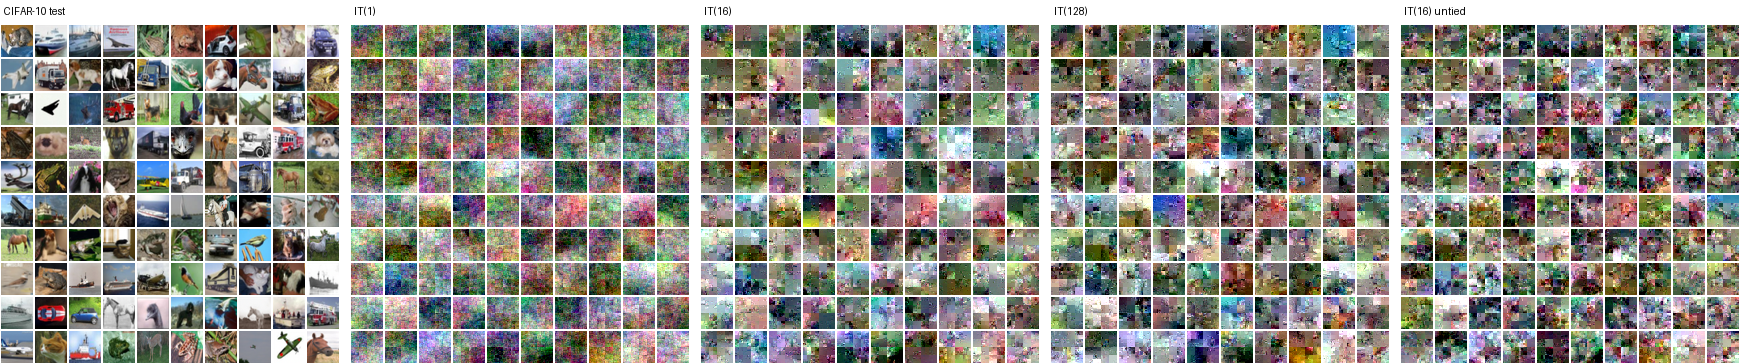
\includegraphics[width=\textwidth]{cifar_samples.png}
\caption{Left: CIFAR-10 test images. Right: samples (top-down, exact ancestral sampling) from the four models of
Table~\ref{tab:cifarmain}, all trained with zero labels.}\label{fig:cifarsamples}
\end{figure}

\subsection{The semantic top: the label as one more child of the root}\label{sec:semtop}
In \S\ref{sec:cifar-res} the label was attached \emph{after} learning: the model was fitted with zero labels and
the label kernel $\ell$ was then fitted on a frozen root. The model of Proposition~\ref{prop:readout} is a
joint one, $p(X,y)$, with $y$ a child of the root. Its maximum-likelihood fit on a mix of labelled and
unlabelled images uses the same generalized EM. The label leaf is observed where it is known and summed out
where it is not. Nothing else is added, so the rule stays pure. Partial tying (\S\ref{sec:partial}) says where
such a top should differ from the rest of the tree. This subsection works out what labels can and cannot
do in that model, before any run.

\begin{definition}[semantic top $\mathrm{ST}(H,c^*)$]\label{def:semtop}
$\mathrm{IT}(H)$ in which the kernels of parents at heights $c\ge c^*$ are untied (one copy per height),
the kernels below $c^*$ are tied, and the label $y\in\{1,\dots,C\}$ is a fifth child of the root with
kernel $\ell(y\mid h_R)$. $c^*=L+1$ is the tied model, and $c^*=1$ the untied one. It is trained by
generalized EM on $N$ images, of which $P$ carry their label.
\end{definition}

\begin{proposition}[price of semantics]\label{prop:price}
Let $\hat\theta_0$ maximize the pixel log-likelihood $\mathcal L_X(\theta)=\sum_n\log p_\theta(X_n)$, and let
$\hat\theta$ maximize the joint log-likelihood $\mathcal L_X(\theta)+\sum_{n\le P}\log p_\theta(y_n\mid X_n)$. Then
\[
0\ \le\ \mathcal L_X(\hat\theta_0)-\mathcal L_X(\hat\theta)\ \le\ \sum_{n\le P}\big(\log C+\log p_{\hat\theta}(y_n\mid X_n)\big)\ \le\ P\log C .
\]
On CIFAR-10 the pixel likelihood lost by learning with all labels is at most
$\log_210/3072=0.0011$ bits/dim.
\end{proposition}
\begin{proof}
Let $\theta_0'$ be $\hat\theta_0$ with the uniform label kernel. Its pixel marginal is that of $\hat\theta_0$, and
$\log p_{\theta_0'}(y\mid X)=-\log C$. The joint optimality of $\hat\theta$ against $\theta_0'$ gives the middle
inequality; the others follow from the optimality of $\hat\theta_0$ and from $\log p(y\mid X)\le0$.
\end{proof}
\noindent This works in both directions. Semantics cost nothing in density. But labels can move the model only
within the set of models whose pixel likelihood is within $H(Y)\le\log C$ nats per labelled image of the
optimum. A class-informative root can be selected by labels only if one already exists among the
near-optimal pixel models. On an image of $3072$ coordinates the label is worth one thousandth of a bit
per coordinate, and it can win only where the pixels are indifferent. The root type is such a place: the
root's own terms are a few bits per image, and they are the only terms that the root type alone decides.

The next statement says how far below the root that indifference extends. For positive vectors $u,u'$ on
the types let $d_H(u,u')=\log\max_h\frac{u(h)}{u'(h)}+\log\max_h\frac{u'(h)}{u(h)}$ (Hilbert's projective
metric; it is unchanged by normalization and by multiplying both vectors by the same positive vector). For a
positive kernel $T$ let $\Delta(T)=\max\log\frac{T[a,b]\,T[a',b']}{T[a,b']\,T[a',b]}$ and
$\kappa(T)=\tanh(\Delta(T)/4)<1$.

\begin{theorem}[label reach]\label{thm:reach}
Fix an image $X$ and a label $y$. Let $q_v$ and $q^y_v$ be the posteriors of the type at node $v$ without and
with the label observed. Let $v$ be at depth $d$ (distance from the root), and let $T^{(1)},\dots,T^{(d)}$ be the
kernels on the edges of its path. Put $\lambda_y=d_H(\ell(y\mid\cdot),\mathbf 1)=\operatorname{osc}_h\log\ell(y\mid h)$
and $\epsilon_v=1-\max_hq_v(h)$. Then
\[
d_H(q^y_v,q_v)\ \le\ D_v:=\lambda_y\prod_{j=1}^d\kappa(T^{(j)}),\qquad
\mathrm{TV}(q^y_v,q_v)\ \le\ \min\Big\{\tanh\frac{D_v}4,\ \frac{\epsilon_v\,e^{D_v}}{1-\epsilon_v}\Big\}.
\]
The joint posterior of $v$ and its parent obeys the bound of the parent ($D_p=D_v/\kappa(T^{(d)})$).
\end{theorem}
\begin{proof}
The posterior of $v$ is $q_v\propto(R_p\,T)\odot a_v$. Here $a_v$ collects $v$'s own emission and the messages
from its children, and $R_p$ is the belief of its parent $p$ without $v$'s message. Only $R_p$ depends on
the label. At the root, $R^y=R\odot\ell(y\mid\cdot)$, so $d_H(R^y,R)=\lambda_y$. A row vector times a positive
kernel contracts $d_H$ by $\kappa(T)$ (Birkhoff--Hopf). Multiplication by $a_v$, and by the messages of $v$'s
other children when passing to the next level, leaves $d_H$ unchanged. Induction down the path gives the
first bound. For probability vectors $\mathrm{TV}\le\tanh(d_H/4)$. For the second form, write
$q^y_v\propto q_v\,r$ with $r(h_0)=1$ at the mode $h_0$ and $r\in[e^{-D_v},e^{D_v}]$. Then
$1-q^y_v(h_0)\le\epsilon_ve^{D_v}/(1-\epsilon_v)$, which bounds the total variation. The joint posterior is
$\propto R_p(h)T[h,h']a_v(h')$, in which only $R_p$ depends on the label, so the same argument applies with $D_p$.
\end{proof}

\begin{corollary}[both rules see the label through the same reach]\label{cor:reach}
(a)~\emph{EM.} On a labelled image, the expected statistics of node $v$ (its type and its parent pair) differ
from those of the same image unlabelled by at most the bound of Theorem~\ref{thm:reach}. The pixel statistics
of every node of every image are label-free.
(b)~\emph{Backpropagation from the root label.} For any parameter $\theta$ of the emissions and transitions,
\[
\partial_\theta\log p(y\mid X)=\sum_v\sum_h\big(q^y_v(h)-q_v(h)\big)\,\partial_\theta\log e_v(h)
+\sum_v\sum_{h,h'}\big(\xi^y_v-\xi_v\big)(h,h')\,\partial_\theta\log T_v[h,h'] ,
\]
with $\xi_v$ the parent--child pair posterior and the root included as $e_R(h)=\pi(h)\,N(t_R;m_h,S_h)$ (Fisher
identity for $p(X,y)$ and $p(X)$). Node $v$ contributes
at most $\mathrm{TV}(q^y_v,q_v)\operatorname{osc}_h\partial_\theta\log e_v(h)$ plus the same for its pair. So
the label signal that reaches a node is the label reach in either rule.
\end{corollary}

\noindent This is the per-image counterpart of Theorem~\ref{thm:labelsignal}. There the root--leaf
correlation decays at rate $q_1$ over the process; here the influence of an observed label decays at rate
$\kappa$ per edge inside the fitted model, and it also vanishes wherever the image already decides the type
($\epsilon_v\to0$). The two rules differ in what else they use. EM also uses the label-free statistics of
every node, and depth multiplies these (claim~1). Backpropagation from labels has only the reach. Three
consequences follow for the design, and each is testable.
\begin{enumerate}
\item \emph{Labels shape the top, and the top is where untying pays.} Below the depth where $D_v$ or
$\epsilon_ve^{D_v}$ is small, labelled and unlabelled images give the same statistics. There, the
kernel is learned from unlabelled data at every height, and tying costs nothing. So $c^*$ should be where
the reach ends, and the untied heights are paid for by Proposition~\ref{prop:wilks}.
\item \emph{Ceiling.} If the kernels below $c^*$ are unchanged by the labels, the root belief, and hence the
Bayes head, is a function of the \emph{state grid} $G_{c^*-1}$. This consists of the thumbnails of the nodes
at height $c^*-1$, which determine every coarser thumbnail and detail, and the messages those nodes receive from
their children. No head of $\mathrm{ST}(H,c^*)$ beats the Bayes accuracy of $y$ from $G_{c^*-1}$. Lowering
$c^*$ raises this ceiling and adds $4^{L-c^*+1}$-fold more untied edges.
\item \emph{Naming.} The root has no context, so its types are named by labels, and only by labels
(Theorem~\ref{thm:ptlower}). The label need is set by the number of top types to name and by the few parameters
of the top that the labels move, not by depth.
\end{enumerate}

\subsection{Calibration and predictions for the semantic top (fixed before the run)}\label{sec:semtop-pred}
\emph{Calibration} (\texttt{verify/exp\_semtop.py cal}, one zero-label tied $\mathrm{IT}(16)$, $3000$ steps, test
$5.120$ bits/dim; Table~\ref{tab:semtopcal}). The fitted kernel is nearly deterministic in the Birkhoff sense:
$\kappa=0.979$--$0.987$ at the four positions. The label kernel fitted on its root has
$\lambda_y=8.5$--$12.1$ nats, and the mean posterior uncertainty is $\epsilon=0.11$--$0.14$ at every height ($0.07$ at
the root). So $D_v\approx9$ at every depth of a CIFAR tree, and \emph{Theorem~\ref{thm:reach} is vacuous on
CIFAR}: it allows a label to change any type in the image. It predicts no decay with depth over four levels, and
we do not claim one. The label's actual reach is measured below, but not predicted.
The class information in the state grids is the other half. An MLP on $G_3$ (the four quadrants: $4\times4$ thumbnail
and their incoming messages) reaches $0.554$, and on $G_2$ ($16$ regions) $0.622$. The zero-label root reaches only
$0.380$ from the same model. The messages add class information beyond the thumbnails at every height, more so
lower down ($+0.05$, $+0.10$, $+0.12$ for linear heads at $c=3,2,1$). \emph{The hidden context types of a zero-label
tree are partly semantic}, and the loss happens at the last merge into the root.

\begin{table}[h]\centering
\caption{Semantic-top calibration: test accuracy of heads (all $50{,}000$ labels, $5000$ held out for model
selection) on the state grid $G_c$ of a zero-label tied $\mathrm{IT}(16)$: thumbnails only, messages only, and
both. The root row uses $(t_R,\log\beta_R)$.}\label{tab:semtopcal}
\small\begin{tabular}{l|c|cc|cc|cc}\toprule
& nodes & \multicolumn{2}{c|}{thumbnails} & \multicolumn{2}{c|}{messages} & \multicolumn{2}{c}{state $G_c$}\\
& & linear & MLP & linear & MLP & linear & MLP\\\midrule
root & 1 & 0.301 & 0.361 & -- & -- & 0.331 & 0.380\\
$c=3$ & 4 & 0.379 & 0.538 & 0.286 & 0.305 & 0.432 & 0.554\\
$c=2$ & 16 & 0.409 & 0.589 & 0.379 & 0.430 & 0.504 & 0.622\\
$c=1$ & 64 & 0.411 & 0.582 & 0.451 & 0.502 & 0.529 & 0.640\\
\bottomrule\end{tabular}
\end{table}

\emph{Run.} $\mathrm{ST}(16,c^*)$ for $c^*=5$ (tied), $4$ (root kernel untied) and $3$ (top two untied), each with
$P=0$, $1000$ and $50{,}000$ labelled images among the $N=50{,}000$, all trained from the same initialization by
generalized EM on the joint likelihood ($3000$ steps). Heads: the joint Bayes head $\sum_h\beta_R(h)\ell(y\mid h)$
with the $\ell$ learned in training; for $P=0$, the post-hoc Bayes head of \S\ref{sec:cifar-res}.
\begin{enumerate}
\item[(S1)] \emph{Price of semantics} (Proposition~\ref{prop:price}). For every $c^*$, the test bits/dim at $P=50{,}000$
and at $P=1000$ are within $0.01$ of those at $P=0$. The bound is $0.0011$ at the optima; $0.01$ is the
optimization noise measured in \S\ref{sec:cifar-claim1}.
\item[(S2)] \emph{Label reach.} The bound of Theorem~\ref{thm:reach} holds at every node (it is a theorem; this checks
the code). No quantitative prediction (see above).
\item[(S3)] \emph{Ceiling} (Corollary~\ref{cor:reach}, item 2). The joint Bayes head stays below the state-grid
estimate plus $0.02$ for the MLP's estimation slack: $\le0.57$ for $c^*=5,4$ and $\le0.64$ for $c^*=3$.
\item[(S4)] \emph{Labels select a semantic root.} The labels move only what the pixels are indifferent to, and the root
type is such a place (Proposition~\ref{prop:price}). So at $P=50{,}000$ the joint Bayes head exceeds the zero-label
post-hoc Bayes head of the same $c^*$ ($0.167$ tied, \S\ref{sec:cifar-res}). The risky part: it exceeds the
zero-label root's best linear head ($0.33$). The labels then produce a root that is more class-informative than any
linear readout of the unlabelled one.
\item[(S5)] \emph{Few labels name, many labels shape.} The pixel side of the root is paid by all $N$ images, and the
label side is gained on $P$ of them. At $P/N=0.02$ the labels cannot reshape the root: the joint Bayes head at $P=1000$
is within $0.03$ of the zero-label model's post-hoc Bayes head with $1000$ labels. Semi-supervised EM with few
labels names the unlabelled types; it does not make new ones.
\item[(S6)] \emph{Untying the top helps the labels.} At $P=50{,}000$ the joint Bayes head is non-decreasing from $c^*=5$
to $4$ to $3$: an untied top can serve the labels without changing the kernel shared by all heights below.
\end{enumerate}

\subsection{Results: the semantic top}\label{sec:semtop-res}
\emph{Run} (\texttt{verify/exp\_semtop.py run}, Colab L4, $10$ minutes for the nine fits).

\begin{table}[h]\centering
\caption{$\mathrm{ST}(16,c^*)$ on CIFAR-10, $N=50{,}000$ images of which $P$ are labelled, joint generalized EM. Test
bits/dim; root heads (joint Bayes head with the $\ell$ learned in training; post-hoc Bayes head and logistic head on
$(\log\beta_R,t_R)$ with $50{,}000$ labels); root belief entropy (nats). Right: measured label reach, the mean
$\mathrm{TV}(q^y_v,q_v)$ over test images (true labels) at each height; Theorem~\ref{thm:reach}'s bound is $0.12$--$0.39$
at every height and was never violated.}\label{tab:semtop}
\small\begin{tabular}{cr|c|ccc|c|ccccc}\toprule
& & & \multicolumn{3}{c|}{root heads} & & \multicolumn{5}{c}{label reach (mean TV)}\\
$c^*$ & $P$ & bits/dim & joint & post-hoc & logistic & entropy & root & $c{=}3$ & 2 & 1 & 0\\\midrule
5 & 0 & 5.120 & -- & 0.176 & 0.338 & 0.15 & & & & &\\
& 1000 & 5.121 & 0.169 & 0.182 & 0.337 & 0.15 & 0.024 & $6\cdot10^{-4}$ & $4\cdot10^{-5}$ & $2\cdot10^{-6}$ & $1\cdot10^{-7}$\\
& 50000 & 5.120 & 0.167 & 0.175 & 0.334 & 0.11 & 0.028 & $2\cdot10^{-3}$ & $1\cdot10^{-4}$ & $5\cdot10^{-6}$ & $2\cdot10^{-7}$\\\midrule
4 & 0 & 5.116 & -- & 0.221 & 0.336 & 0.29 & & & & &\\
& 1000 & 5.113 & 0.189 & 0.211 & 0.344 & 0.25 & 0.031 & $2\cdot10^{-3}$ & $1\cdot10^{-4}$ & $7\cdot10^{-6}$ & $5\cdot10^{-7}$\\
& 50000 & 5.109 & \textbf{0.247} & 0.242 & 0.339 & 0.32 & 0.068 & $4\cdot10^{-3}$ & $2\cdot10^{-4}$ & $1\cdot10^{-5}$ & $8\cdot10^{-7}$\\\midrule
3 & 0 & 5.130 & -- & 0.226 & 0.348 & 0.30 & & & & &\\
& 1000 & 5.117 & 0.210 & 0.229 & 0.356 & 0.31 & 0.032 & $1\cdot10^{-3}$ & $7\cdot10^{-5}$ & $3\cdot10^{-6}$ & $2\cdot10^{-7}$\\
& 50000 & 5.115 & \textbf{0.252} & 0.252 & 0.355 & 0.37 & 0.068 & $4\cdot10^{-3}$ & $2\cdot10^{-4}$ & $9\cdot10^{-6}$ & $5\cdot10^{-7}$\\
\bottomrule\end{tabular}
\end{table}

\paragraph{Reading Table~\ref{tab:semtop}.}
(S1)~\emph{Confirmed in substance, with one margin missed in the harmless direction.} Labels never cost density: the
largest increase is $0.002$ bits/dim ($c^*=5$, $P=1000$), inside the theorem's $0.0011$ plus noise. At $c^*=3$ the
labelled fits are $0.013$--$0.015$ \emph{better} than the zero-label fit, which is outside the stated $0.01$. That
zero-label fit is simply a worse optimum ($c=2$ and $c=3$ bits are both worse), so the optimization noise of the more
untied model is larger than the $0.01$ measured for the tied one.
(S2)~\emph{Confirmed} (no violation at any node). See below for what the measured reach shows.
(S3)~\emph{Confirmed, but not binding}: every head is far below the ceilings ($0.57$, $0.64$).
(S4)~\emph{Refuted for the tied model, confirmed for the untied tops, and the risky part refuted.} With all labels, the
tied model's joint head is $0.167$, no better than its zero-label post-hoc head. The untied tops gain: $0.221\to0.247$ at
$c^*=4$ and $0.226\to0.252$ at $c^*=3$. No joint head approaches the $0.33$ of a linear readout of the unlabelled root.
(S5)~\emph{Confirmed.} At $P=1000$ the joint head is within $0.003$--$0.016$ of the zero-label post-hoc head, and always
below it. Few labels name; they do not shape.
(S6)~\emph{Confirmed}: $0.167\le0.247\le0.252$.

\emph{Why (S4) failed: the premise was wrong, and the calibration already showed it.} Proposition~\ref{prop:price} says
labels can move only what the pixels are indifferent to. We assumed the root type was such a place. It is not: the
root belief has entropy $0.11$--$0.37$ nats, so the pixels (the root thumbnail and the four quadrant types) already
decide the root type with a margin of several nats per image. The label pays at most $\lambda_y$, and the learned label
kernels have $\lambda_y\approx1$--$3$ nats: the label kernel is fitted to root types that are not class-pure, and so it
cannot pay for making them purer. This is a self-consistent fixed point of joint EM, and the calibration's root entropy
($0.15$) was the number that should have predicted it. Per image the statement is: an image's root type can follow
its label only if its pixel margin between root types is below the label kernel's spread. Pure likelihood with the label
as a root child therefore cannot create semantics at a root that the pixels have already decided. Untying the top
loosens the root (entropy $0.15\to0.3$), and only then do the labels move it a little.

\emph{What the measured reach shows.} The label's influence falls by a factor of $15$--$25$ per level: from
$\mathrm{TV}\approx0.03$--$0.07$ at the root to $\approx10^{-7}$ at the $2\times2$ patches. In $d_H$ the per-edge ratio is
$0.03$--$0.06$, nearly constant with depth (for $c^*=5$, $P=50{,}000$: $2.9$, $0.10$, $0.0055$, $0.00028$, $1.4\cdot10^{-5}$). The
kernel's own Birkhoff constant is $\kappa\approx0.98$, so the contraction does not come from the kernel. It comes from
the certainty of the parent. If the parent's belief $R$ puts mass $1-\epsilon$ on a type $h_0$ and the label multiplies
it by weights within $e^{\pm d}$, then with $\rho=\max_{h,h'}T[h,h']/T[h_0,h']$,
\[
d_H(R^yT,\,RT)\ \le\ \log\frac{1+e^{d}a}{1+e^{-d}a},\qquad a=\frac{\epsilon\rho}{1-\epsilon},
\]
which is $\approx2\sinh(d)\,a$ for small $a$: the downward perturbation is damped by the parent's uncertainty
$\epsilon\approx0.1$ (proof: only the non-modal part of $R$ is reweighted relative to the mode, and it enters $RT$ with
weight at most $a$ relative to the modal row). We did not measure $\rho$, so the constant is not checked; the mechanism
matches the observed order of magnitude. For claim~2 this is Corollary~\ref{cor:reach}(b) measured: \emph{per image,
the root label's signal reaching a node falls about twentyfold per level on CIFAR}, so even summed over the $4^d$ nodes
at depth $d$ it falls about fivefold per level. Backpropagation from root labels can teach, on its own, only the top one
or two levels of this tree. Below that, the kernel must come from unlabelled data, which is what tying and claim~1
provide.

\emph{What the semantic top teaches.} The class information is present in the zero-label tree ($0.55$ and $0.62$ from
the state grids at $c=3$ and $2$, with the hidden types contributing beyond the thumbnails) and is lost at the last
merge, where a near-certain discrete root type is chosen by pixel likelihood. Labels observed at that root, with
the pure joint likelihood, cannot get it back: they are too weak against a decided root, and too weak to reach below
it. The theory now says what a semantic top needs. Its state must stay uncertain enough under the pixels, meaning a
margin below $\lambda_y$, for labels to shape it. It must also carry the grid's information into the root rather than
a single type chosen by pixels. Both are properties of the top's state space, not of the learning rule.

\subsection{A context for the root: views of one scene}\label{sec:views}
\emph{Diagnosis.} Every hidden type below the root is shaped by its context: it must carry what its siblings and
parent need (Theorem~\ref{thm:mng}, Proposition~\ref{prop:hidden}). The root has no context. Its type is paid only
by its own children: it is whatever makes the root thumbnail and the four quadrant states conditionally independent.
Pixel likelihood spends it on the largest such dependence, which on CIFAR is the global look of the image. The
calibration shows this: the root type adds $0.02$--$0.03$ to the class accuracy of the whole image's $2\times2$ colour
thumbnail (Table~\ref{tab:semtopcal}). There are two further defects: the root sees the image only through a
$16$-way merge of four near-certain quadrant types, and a tied root means what a pixel patch means. A label cannot
repair this. It is a context worth at most $\log C$ per image, and the model can neutralize it at no pixel cost
(Proposition~\ref{prop:price}). The root needs a context made of pixels.

\begin{definition}[scene grammar $\mathrm{SG}(H,M)$ with $K$ views]\label{def:sg}
A scene type $z\in\{1,\dots,M\}\sim\pi$ is the common parent of $K$ views, each a whole image tree. Every node of a view
has state $(t,h,z)$, with $z$ copied from parent to child (parent-determined and hidden). Given $z$, a view is
$\mathrm{IT}(H)$ with root prior $\pi_z(h)$ and type kernel $T_{z}$ (tied across heights); the emissions are shared by all
$z$. So $z$ selects a grammar over shared types, and the types are its words. The label, when observed, is a child of the
scene node with kernel $\ell(y\mid z)$. Given $z$ the views are independent trees, so sum--product is exact at $M$ times
the cost of the type passes. With one view the scene node is a mixture over $M$ tied grammars.
\end{definition}

\noindent The scene type sees a view through its whole tree: $\log P(z\mid X)=\log\pi(z)+\log p_z(X)+\mathrm{const}$, and
$\log p_z(X)$ sums the transition evidence of all $340$ edges. There is no $16$-way merge at the top, which removes the
second defect. The first defect is what the views are for.

\begin{proposition}[agreement identity]\label{prop:agree}
For $K$ views and $w_k(z)=P(z\mid X^k)$, the single-view posteriors under the same model,
\[
\log p(X^1,\dots,X^K)=\sum_k\log p(X^k)+\underbrace{\log\sum_z\pi(z)\prod_k\frac{w_k(z)}{\pi(z)}}_{\text{agreement}} .
\]
With the label as a view ($p(y\mid z)=\ell(y\mid z)$), the agreement term is $\log\sum_zw(z)\ell(y\mid z)=\log p(y\mid X)$.
\end{proposition}
\begin{proof}
$p(X^1,\dots,X^K)=\sum_z\pi(z)\prod_kp_z(X^k)$, and $p_z(X^k)=w_k(z)p(X^k)/\pi(z)$ by Bayes.
\end{proof}

\begin{corollary}[leverage of a context]\label{cor:leverage}
(a)~\emph{Label.} Setting $\ell$ uniform makes the agreement term $-\log C$, whatever $z$ does, at no pixel cost. So a label
can move $z$ by at most $\log C$ per labelled image, and the model can refuse it cheaply. This is what happened in
\S\ref{sec:semtop-res}, where the learned $\ell$ had $\lambda_y\approx1$--$3$ nats.
(b)~\emph{Views.} The agreement term is at most $(K-1)\log(1/\min_z\pi(z))$, and it is attained when the views' posteriors
agree and are sharp. If the views' posteriors are sharp but disagree, it is about minus the smaller evidence margin,
without bound. The model has only two ways out. Either $z$ is a function of what the views share, or $z$ is
uninformative ($w_k=\pi$), which gives up the whole single-view gain of the mixture. So views can move $z$ by up to the
entire value of $z$ to the pixels.
\end{corollary}
\begin{proof}
(a) $\log\sum_zw(z)/C=-\log C$. (b) $\sum_z\pi\prod_k(w_k/\pi)\le\max_z\pi(z)^{-(K-1)}\sum_zw_1(z)\le\min_z\pi(z)^{-(K-1)}$.
If $w_1$ and $w_2$ put mass $\ge1-\epsilon$ on different types, the sum is at most $2\epsilon/\min\pi$, and
$\log\epsilon$ is minus the evidence margin.
\end{proof}

\noindent What $z$ becomes, if it agrees across views, is fixed by the view family.

\begin{theorem}[the scene type is the view invariant]\label{thm:invariant}
Let $S$ be a random scene, $g_1,g_2,\dots$ i.i.d.\ from $\nu$ and independent of $S$, and $X^k=g_k\cdot S$. Let $O(S)$ be
the law of $g\cdot S$ given $S$. Then:
(a) the views are conditionally i.i.d.\ given $O(S)$;
(b) if some latent $Z$ makes them conditionally i.i.d.\ with law $Q_Z$, then $Q_Z=O(S)$ almost surely: the views
determine $O(S)$, and a scene type distinguishes nothing finer than $O(S)$;
(c) if $\nu$ is Haar measure on a compact group $G$ acting on scenes, then $O(S)=O(S')$ iff $S'\in G\cdot S$: the scene
type is the $G$-orbit, the content of the scene that the transformations do not change.
\end{theorem}
\begin{proof}
(a) Given $S$, the $g_k$ are i.i.d. (b) The empirical measure of $X^1,\dots,X^n$ converges almost surely (on a countable
convergence-determining class) to $Q_Z$, because the views are conditionally i.i.d.\ given $Z$, and to $O(S)$ by (a).
(c) If $S'=h\cdot S$ then $g\cdot S'=(gh)\cdot S$, which has the law of $g\cdot S$ by invariance of Haar measure.
Otherwise the two laws live on the disjoint closed orbits $G\cdot S$ and $G\cdot S'$.
\end{proof}

\noindent With finitely many scene types, maximum likelihood chooses among partitions of the invariant content: the
agreement term (Corollary~\ref{cor:leverage}) requires $z$ to be (nearly) a function of $O(S)$, and the single-view term
picks, among such functions, the one worth the most pixels. Three consequences follow, each testable.
\begin{enumerate}
\item \emph{The family decides the semantics.} Crops and flips leave the global colour shared, so $z$ may carry it. With
independent colour jitter, colour is not shared, and $z$ must drop it. Class enters $z$ only as part of the invariant,
and only if it is worth pixels. The theory does not promise that it is; it says this is the only route.
\item \emph{Depth adds data at the top.} The scene node has $K$ children, so its kernel is learned from $K$ views per
scene, as every other node's is learned from its siblings (Theorem~\ref{thm:depthg}).
\item \emph{Labels only name.} With $z$ fixed by the views, labels fit $\ell$, which has $M(C-1)$ numbers
(Theorem~\ref{thm:ptlower}).
\end{enumerate}

\paragraph{Predictions (fixed before the run).} Models, all with zero labels on the $50{,}000$ training images: R, the
tied $\mathrm{IT}(16)$ (the old root); A, $\mathrm{SG}(16,16)$ with one view and no transformation (no merge bottleneck,
no context); B, two views under random crops (4-pixel reflect padding) and flips; C, two views under crops, flips and
independent colour jitter (brightness, contrast, saturation, channel gains, $20\%$ grey); D, as C with four views.
$3000$ steps of $128$ scenes each. The state of a test image is its single-view posterior $w(z)$ (R: the root belief).
\begin{enumerate}
\item[(W1)] \emph{Agreement produces invariance} (Corollary~\ref{cor:leverage}, Theorem~\ref{thm:invariant}). The mean
$\mathrm{TV}(w(gX),w(X))$ under random crops and flips is at most half of A's for B, C and D. Under colour jitter it is at
most half of B's for C and D.
\item[(W2)] \emph{The family decides the semantics.} The $R^2$ of an image's mean colour from its state is at most half
as large for C as for B.
\item[(W3)] \emph{Without context the root stays a pixel clustering.} A's state carries the global look (colour
$R^2$ at least that of R), and its post-hoc Bayes head is at most $0.28$: removing the merge alone does not make the
root semantic.
\item[(W4)] \emph{Density.} A contains R ($M=1$), so A's test bits/dim is at most R's $+0.01$.
\item[(W5)] \emph{Class, the risky one.} With all labels naming the scene types, the Bayes head of C is at least that of
B, at least $0.30$ (above every root so far, $\le0.25$), and D's is at least C's.
\item[(W6)] \emph{Labels only name.} For B, C, D the Bayes head with $1000$ labels is within $0.02$ of that with
$50{,}000$.
\end{enumerate}

\subsection{Results: views of one scene}\label{sec:views-res}
\emph{Run} (\texttt{verify/scenetree.py}, \texttt{verify/exp\_views.py}; checks in \texttt{verify/test\_scenetree.py}:
brute force, Fisher identity for $K=1,2,3$ with and without labels, the agreement identity, and $M=1$ equal to
$\mathrm{IT}$; Colab L4, $12$ minutes). One change was made after the predictions were fixed and before the run: a smoke test
showed one scene type taking $99\%$ of the images at initialization, and a mixture component that starts with no
responsibility never receives a gradient. The $M$ kernels therefore start from a shared kernel plus a small ($0.005$) per-type
perturbation, which gives every type about $1/M$ of the images at the start.

\begin{table}[h]\centering
\caption{Views of one scene, CIFAR-10, zero labels in training. Types used: scene types with $\ge5\%$ of the test images.
Heads on the state: post-hoc Bayes with $10^3$ and $5\cdot10^4$ labels, logistic on the state, and logistic on the state
and the root thumbnail. Invariance: mean $\mathrm{TV}(w(gX),w(X))$ for crops and flips, for colour jitter, and between two
different images (scale). Colour: $R^2$ of the image's mean colour from the state (D: least squares ill-conditioned, not
reported).}\label{tab:views}
\small\begin{tabular}{l|c|c|cc|cc|c|ccc|c}\toprule
& types & & \multicolumn{2}{c|}{Bayes} & \multicolumn{2}{c|}{logistic} & & \multicolumn{3}{c|}{invariance TV} & colour\\
model & used & bits/dim & $10^3$ & $5{\cdot}10^4$ & state & $+t_R$ & entropy & crop & colour & other & $R^2$\\\midrule
R: $\mathrm{IT}(16)$ root & 2 & 5.120 & 0.166 & 0.176 & 0.294 & 0.337 & 0.15 & 0.087 & 0.231 & 0.421 & 0.945\\
A: $K=1$ & 3 & 5.108 & 0.190 & 0.190 & 0.230 & 0.349 & 0.03 & 0.141 & 0.216 & 0.647 & 0.126\\
B: $K=2$, crop & 3 & 5.114 & 0.190 & 0.190 & 0.235 & 0.347 & 0.04 & 0.154 & 0.237 & 0.665 & 0.127\\
C: $K=2$, crop+colour & 2 & 5.128 & 0.148 & 0.154 & 0.185 & 0.316 & 0.01 & 0.054 & 0.119 & 0.341 & 0.128\\
D: $K=4$, crop+colour & 2 & 5.119 & 0.152 & 0.158 & 0.200 & 0.324 & 0.01 & 0.065 & 0.105 & 0.394 & --\\
\bottomrule\end{tabular}
\end{table}

\paragraph{Reading Table~\ref{tab:views}.}
(W1)~\emph{Refuted in substance.} B is no more crop-invariant than A ($0.154$ against $0.141$). C and D pass the stated
test (crop TV $0.054$, $0.065$ against A's $0.141$; D's colour TV $0.105$ against B's $0.237$; C's $0.119$ misses by $0.001$).
But they do it by using fewer types: relative to the TV between two different images, the invariance of C and D is no better
than B's (colour: $0.35$, $0.27$ against $0.36$).
(W2)~\emph{Not a test.} No scene state carries colour ($R^2\approx0.13$ for A, B and C). In this design colour lives in
the root type of each view, not in $z$, so the prediction could not discriminate.
(W3)~\emph{Half refuted.} A's state does not carry the global look ($R^2=0.13$, against $0.945$ for the old root). Its Bayes
head is $0.190\le0.28$, as predicted.
(W4)~\emph{Confirmed}: A $5.108$ against R $5.120$.
(W5)~\emph{Refuted.} C ($0.154$) is below B ($0.190$), far below $0.30$, and D equals C.
(W6)~\emph{Confirmed, trivially}: with two or three types in use there is little to name.

\emph{What happened, and what it says about the root.}
(i)~\emph{The old root is a colour code.} Its state predicts the image's mean colour with $R^2=0.945$ and uses essentially
two of its sixteen types ($73\%$ and $21\%$ of the images). This confirms the diagnosis at the start of \S\ref{sec:views}
directly.
(ii)~\emph{A global discrete variable is decided by hundreds of nats.} Once $z$ sees every edge, its single-view posterior
has entropy $0.01$--$0.04$ nats. Generalized EM on such hard posteriors keeps the few components that win early: two or
three of sixteen in every run. The near-symmetric start delays this but does not prevent it.
(iii)~\emph{The views pruned; they did not create.} Corollary~\ref{cor:leverage}(b) gives the model two ways out of
disagreement: an invariant $z$, or an uninformative one. With colour jitter the model took the second, keeping two scene
types. We had argued that this exit is expensive because it gives up the single-view gain of the mixture. That gain turned
out to be small: A is only $0.012$ bits/dim better than R. Views can remove distinctions that are not shared, but they
cannot make the likelihood want a distinction, such as the class, that is worth few pixels. Theorem~\ref{thm:invariant} says
what $z$ may be; the single-view term decides what it is, and on CIFAR it prefers very little.
(iv)~\emph{Where the class is.} Linear heads on the zero-label state grids reach $0.43$, $0.50$, $0.53$ at $c=3,2,1$
(Table~\ref{tab:semtopcal}), against $0.39$ for a linear head on the raw pixels: the unlabelled tree's region states are
better linear features than pixels. Every attempt to push this into \emph{one} variable at the top, whether a root type, a
labelled root, or a scene type shared by views, has produced a coarse clustering by bulk statistics. The class is carried by
the \emph{configuration} of region states, and a strong root must keep that configuration rather than choose among a few
pixel prototypes.

\subsection{A root that keeps the configuration: the state grid}\label{sec:grid}
Every failure above has the same cause: some variable at the top was chosen by pixel likelihood, and the pixels chose
bulk statistics. The alternative is to choose \emph{nothing} by pixel likelihood above some height $c$. Below $c$, every
node has context (siblings and a parent), and the zero-label tree is what the theory says it should be. Above $c$, the
class reads the whole grid of region states.

\begin{definition}[grid-parent model $\mathrm{GP}(c)$]\label{def:gp}
Keep the tied tree below height $c$. Replace everything above by the class: $y\sim p(y)$, and given $y$ the $n_c=4^{L-c}$
nodes $v$ at height $c$ are independent, with type $h_v\sim\rho_v(h\mid y)$ and thumbnail $t_v\sim N(\mu_{v,y},\Sigma_v)$.
The head is \emph{untied} if $\rho_v,\mu_v,\Sigma_v$ depend on the position $v$, and \emph{tied} if they do not.
\end{definition}

\begin{proposition}[grid readout]\label{prop:gridread}
Let $e_v(h)=p(X_{<v}\mid h_v=h,t_v)$ be the message that grid node $v$ receives from its subtree (computed by the
zero-label tree), and $\tilde e_v=e_v/\sum_he_v(h)$. Under $\mathrm{GP}(c)$,
\[
\log P(y\mid X)=\log p(y)+\sum_v\Big[\log\sum_h\rho_v(h\mid y)\,\tilde e_v(h)+\log N(t_v;\mu_{v,y},\Sigma_v)\Big]+\mathrm{const}(X).
\]
If $\tilde e_v$ puts mass $1-\epsilon_v$ on one type $h^*$, then
$0\le\log\sum_h\rho_v(h\mid y)\tilde e_v(h)-\sum_h\tilde e_v(h)\log\rho_v(h\mid y)\le\log\big(1+\epsilon_v\tfrac{\max\rho}{\rho(h^*)}\big)
+\epsilon_v\log\tfrac{\rho(h^*)}{\min\rho}$. So, up to that error, the Bayes log-odds are \emph{linear} in the features
$(\tilde e_v,t_v)_v$: a linear head on the grid is the Bayes rule of $\mathrm{GP}(c)$.
\end{proposition}
\begin{proof}
Given $y$ the grid nodes are independent, and below each of them the tree is the zero-label tree, so
$p(X\mid y)=\prod_v\sum_h\rho_v(h\mid y)N(t_v;\mu_{v,y},\Sigma_v)\,e_v(h)$. Normalizing $e_v$ changes only a factor
that does not depend on $y$. The quadratic terms in $t_v$ cancel between classes because $\Sigma_v$ is shared. The lower
bound is Jensen's inequality. For the upper bound, the sum is at most $\rho(h^*)+\epsilon_v\max\rho$, and
$\sum_h\tilde e_v\log\rho\ge(1-\epsilon_v)\log\rho(h^*)+\epsilon_v\log\min\rho$.
\end{proof}

\noindent Nothing above height $c$ is chosen by pixels, so the failure of \S\ref{sec:semtop-res} and
\S\ref{sec:views-res} cannot occur. The labels choose which regions, which types and which colours matter. The price is that
labels now fit more numbers than a root kernel.

\begin{corollary}[who pays for what]\label{cor:gridcost}
(a)~\emph{Labels.} The untied head has $d_c=n_c(H+12)(C-1)$ free numbers, and its expected excess log-loss from $P$ labels is
$\approx d_c/(2P)$ (Proposition~\ref{prop:wilks}). So its label need grows fourfold per level of refinement. The tied head has
$d=(H+12)(C-1)$ at every $c$, since it reads the grid as a bag of region states and gives up position. This is
self-similarity applied to the readout.
(b)~\emph{Unlabelled images.} The features $(\tilde e_v,t_v)$ are made by the zero-label tied kernel, which $\approx10^3$
unlabelled images already fix (\S\ref{sec:cifar-claim1}). So the readout's accuracy is fixed by $\approx10^3$ unlabelled images
as well (claim~1, now for classification).
(c)~\emph{Same architecture, two rules} (claim~2). Local EM learns the kernel from unlabelled images, and labels fit only
the head. Backpropagation of the label loss through the same tree must also learn the kernel ($26{,}032$ numbers) from the
labels, and the label's signal reaches the nodes below the grid only through the label reach, which fell about twentyfold per
level on CIFAR (\S\ref{sec:semtop-res}).
\end{corollary}

\paragraph{Predictions (fixed before the run).} Features from the zero-label tied $\mathrm{IT}(16)$ ($3000$ steps, $N$
unlabelled images), at $c=3,2,1$ ($4$, $16$, $64$ regions). Heads: untied and tied logistic (conditional maximum
likelihood of $\mathrm{GP}(c)$), and the generative $\mathrm{GP}(c)$ fit by maximum likelihood (the Bayes grid head:
$\rho_v(h\mid y)$ from soft counts of $\tilde e_v$, class means and a pooled covariance for $t_v$). Labels
$P\in\{100,300,10^3,3\cdot10^3,10^4,5\cdot10^4\}$. $P_{0.02}$ denotes the smallest of these at which a head is within $0.02$ of
its own accuracy at $P=5\cdot10^4$.
\begin{enumerate}
\item[(G1)] \emph{Label need grows with the grid} (Corollary~\ref{cor:gridcost}(a)). For the untied logistic head,
$P_{0.02}$ is non-decreasing from $c=3$ to $2$ to $1$; at $c=3$ it is at most $10^4$, and at $c=1$ it is $5\cdot10^4$
($d_1=17{,}920$).
\item[(G2)] \emph{The tied head is label-cheap.} At every $c$ its $P_{0.02}$ is at most $3000$.
\item[(G3)] \emph{Depth adds data to the readout} (Corollary~\ref{cor:gridcost}(b)). The untied head at $c=2$ with all
labels, on features from $N=1024$ unlabelled images, is within $0.02$ of the same head on features from $N=50{,}000$.
\item[(G4)] \emph{Claim~2} (Corollary~\ref{cor:gridcost}(c)). At $c=2$, EM features with the untied logistic head against
backpropagation of the cross-entropy through the same tree and head from the same initialization (learning rate best of
three on $5000$ held-out labelled images, early stopping on them, neither counted in $P$). EM is at least as accurate at
every $P\le10^4$, and ahead by at least $0.05$ at $P=1000$.
\item[(G5)] \emph{The grid beats the root, even generatively.} The Bayes grid head at $c=2$ with all labels exceeds $0.30$,
above every Bayes head on a single top variable so far ($\le0.25$).
\end{enumerate}

\subsection{Results: the state grid}\label{sec:grid-res}
\emph{Run} (\texttt{verify/exp\_grid.py}, Colab L4, $12$ minutes).

\begin{table}[h]\centering
\caption{Readouts of the zero-label tied $\mathrm{IT}(16)$'s state grid, CIFAR-10 test accuracy against the number of labels
$P$. Features from $N=50{,}000$ unlabelled images. Last row: backpropagation of the cross-entropy through the same tree and
untied head ($c=2$) from the same initialization, learning rate best of three and early stopping on $5000$ further labelled
images; its largest $P$ is $45{,}000$.}\label{tab:grid}
\small\begin{tabular}{ll|cccccc}\toprule
& head & $P=100$ & 300 & $10^3$ & $3\cdot10^3$ & $10^4$ & $5\cdot10^4$\\\midrule
$c=3$ (4 regions) & untied & 0.221 & 0.232 & 0.318 & 0.387 & 0.420 & 0.434\\
& tied & 0.199 & 0.245 & 0.313 & 0.336 & 0.339 & 0.341\\
& Bayes grid & 0.247 & 0.319 & 0.362 & 0.377 & 0.384 & 0.386\\\midrule
$c=2$ (16 regions) & untied & 0.243 & 0.290 & 0.336 & 0.379 & 0.462 & \textbf{0.505}\\
& tied & 0.214 & 0.286 & 0.333 & 0.351 & 0.360 & 0.365\\
& Bayes grid & \textbf{0.259} & \textbf{0.337} & \textbf{0.382} & 0.396 & 0.403 & 0.409\\\midrule
$c=1$ (64 regions) & untied & 0.249 & 0.342 & 0.366 & 0.388 & 0.419 & \textbf{0.525}\\
& tied & 0.225 & 0.306 & 0.364 & 0.380 & 0.394 & 0.388\\
& Bayes grid & 0.239 & 0.337 & 0.370 & 0.389 & 0.397 & 0.407\\\midrule
$c=2$ & backprop & -- & 0.283 & 0.373 & \textbf{0.425} & \textbf{0.475} & 0.483\\
\bottomrule\end{tabular}
\end{table}

\paragraph{Reading Table~\ref{tab:grid}.}
(G1)~\emph{Confirmed.} The untied head's $P_{0.02}$ is $10^4$ at $c=3$ and $5\cdot10^4$ at $c=2$ and $c=1$: the finer the grid,
the more labels, as $d_c$ says.
(G2)~\emph{Confirmed.} The tied head is within $0.02$ of its limit at $P=3000$ at every $c$. It pays for this with a lower
limit ($0.34$--$0.39$): position matters.
(G3)~\emph{Confirmed.} Features from $1024$ unlabelled images give $0.496$ at $c=2$, against $0.505$ from $50{,}000$. Claim~1
holds for classification: the unlabelled data a readout needs are fixed by the tied kernel, and $10^3$ images suffice.
(G5)~\emph{Confirmed.} The Bayes grid head reaches $0.41$ at $c=2$, against $\le0.25$ for every single top variable. It is
also the most label-efficient readout: $0.34$ with $300$ labels and $0.38$ with $1000$.
(G4)~\emph{Refuted.} Backpropagation through the same architecture is behind at $P=300$ ($0.283$, against $0.290$ for the
untied head and $0.337$ for the Bayes grid head). It leads from $P=1000$ to $10^4$ by up to $0.05$ ($0.425$ against
$0.379$--$0.396$ at $3000$), and it is behind again with all labels ($0.483$ against $0.505$; with $3000$ steps it may be
under-trained there). Backprop also had $5000$ extra labels for learning-rate choice and early stopping, which the EM heads did
not use; the refutation stands without that.

\emph{Why (G4) failed: tying shortens the label's path for backpropagation too.} Corollary~\ref{cor:gridcost}(c) argued
from the label reach: the signal of the label falls about twentyfold per level below it. That is true per node. But the
kernel is tied, so backpropagation needs to reach only the \emph{first} level below the grid. Every level's edges update the
same kernel, and the nearest edges carry an undamped label signal. With the grid at $c=2$ that is one edge away. The decay
argument (and Theorem~\ref{thm:labelsignal}) constrains backpropagation for untied deep parameters, or for labels far
above the parameters they must teach; it does not apply to a tied kernel read at a grid just above it. Once the labels
number in the thousands, backpropagation then gets what EM does not: types chosen for the class rather than for the pixels.
The zero-label kernel spends its sixteen types on explaining pixels, and a linear head on them saturates at $0.38$--$0.40$
for $P\le3000$.

\emph{What this settles.} The strong root is the grid, and it can be built without labels: $0.51$--$0.53$ linear and $0.41$
generative, from features that $10^3$ unlabelled images fix. That is well above every root variable ($\le0.38$), and
above a linear head on raw pixels ($0.39$). Labels are needed only for the head, and the generative head is best when
labels are few. Claim~2, in its strong form on CIFAR, does not hold for this architecture. Local EM beats backpropagation
only below about $10^3$ labels. Between $10^3$ and $10^4$, backpropagation through the same tied tree uses the labels
better, because it makes class-relevant types and tying brings the label within one edge of the kernel. The advantage
of the local rule on CIFAR is claim~1: zero labels and $10^3$ images for the representation.

\subsection{What a label can buy, wherever it sits}\label{sec:labelworth}
The natural pure repair is to make the label the \emph{parent} of the grid in a joint model, $\mathrm{GP}(c)$ above a
tied tree, and fit everything by EM on labelled and unlabelled images together. The label would then vote on
$n_c$ region types instead of one root type. The theory rules this out before it is built.

\begin{proposition}[a label is worth at most $\log C$, wherever it sits]\label{prop:labelworth}
For any joint model $p_\theta(X,y)$, whatever the position of $y$, let $\hat\theta$ maximize the joint log-likelihood on
$N$ images of which $P$ are labelled, and let $\hat\theta_0$ maximize the pixel log-likelihood. Then
$\mathcal L_X(\hat\theta_0)-\mathcal L_X(\hat\theta)\le P\log C$: the joint optimum is within $(P/N)\log C$ nats per image of a
pixel-optimal model.
\end{proposition}
\begin{proof}
$\log p(X,y)=\log p(X)+\log p(y\mid X)$ for every model, so the joint log-likelihood is the pixel log-likelihood plus the
conditional log-likelihood of the labels. The argument of Proposition~\ref{prop:price} applies unchanged.
\end{proof}

\begin{corollary}[when a generative rule can beat a discriminative one]\label{cor:genvsdisc}
The classifier of the joint optimum is the best one among models within $(P/N)\log C$ nats per image of the pixel optimum.
If the class is a function of the pixel-optimal state, it reaches the Bayes rule from few labels, whatever the depth.
This is the tied grammar, where the class is the root of the context-optimal state (Theorem~\ref{thm:mng}), and the local rule
wins exponentially in depth (\S\ref{sec:claim2}). If the class is not such a function, labels cannot move the representation
toward it by more than $(P/N)\log C$ per image. A rule that ignores the pixels (conditional likelihood only) has no such cap
and pays only in label variance.
\end{corollary}

\noindent On CIFAR with $P=1000$ of $N=50{,}000$, the cap is $0.046$ nats per image. Moving the class-mixture of
$\mathrm{GP}(c)$ from the pixel-optimal partition (colour and texture, \S\ref{sec:views-res}) to the class costs far more, and
so would sharpening the band of types below the grid. So the label-as-parent joint EM is predicted to equal the two-stage
readout of \S\ref{sec:grid-res} at small $P$, and to lose to backpropagation between $10^3$ and $10^4$ labels. We do not run
it.

\begin{proposition}[the label gradient is local]\label{prop:localgrad}
In any tree model with the label as a node, $\partial_\theta\log p(y\mid X)$ is the difference of the grid-local expected
statistics with the label clamped and with it free (Corollary~\ref{cor:reach}(b)). Two sum--product passes compute it, each
node using only its own posterior and its parent pair.
\end{proposition}

\noindent So on a tree, ``backpropagation from labels'' and ``local learning'' do not differ in locality: conditional
maximum likelihood is itself a clamped-minus-free local rule. They differ in what they learn from. The only resource a local
rule has beyond the labels is the unlabelled data, and Proposition~\ref{prop:labelworth} bounds what a generative objective can
extract from it for a class that the pixels do not favour. On such data, claim~2 reduces to two estimators in sequence. First,
maximum likelihood on the unlabelled images fixes the representation (claim~1: $10^3$ images). Second, conditional maximum
likelihood by the clamped-minus-free rule refines it from the labels. The comparison with backpropagation from scratch is then
a comparison of starting points on the same objective. (The head-to-head of \S\ref{sec:grid-res} used a discriminative
linear head on the messages rather than the generative head of $\mathrm{GP}(c)$. Its gradient also travels only along tree
edges, but it is not literally the clamped-minus-free difference.)

%==========================================================================
\section{Discussion and what remains open}
%==========================================================================
\paragraph{What the symmetry buys.}
In the untied model the top level is a grid without context, so labels are necessary
(Theorem~\ref{thm:lower}). Tying the rules lets the top level borrow the bottom level's context:
the $s^{L-1}$ bottom grids of a single example are $s^{L-1}$ conditionally independent views of
the same local problem. This is the formal version of the notes' ``the substrate is identical,
so a strategy learned at one level transfers to all''. The learning rule is not gradient-based.
It is the statistical Myhill--Nerode quotient (merge grids no context can distinguish), followed
by naming through self-consistency across scales.

\paragraph{Limitations.}
(i)~Theorem~\ref{thm:rec} assumes a non-degenerate realized histogram; Prop.~\ref{prop:neff}
certifies this only via a conservative worst-case $\lambda$. (ii)~Brute-force naming costs
$v!$. Constraint propagation (as in isomorphism testing of random structures) should be
polynomial on typical instances, but we have not proved it. (iii)~The RHM is noise-free and
unambiguous. Noisy or ambiguous grammars need the soft version (belief propagation;
srg.pdf, \S5). (iv)~Experiments use one small configuration.

\begin{problem}[a lower bound for backprop on the tied model; partly addressed in \S\ref{sec:claim2}]
Show that SGD on a deep CNN with root labels (tied or untied weights) needs a number of labelled
examples growing with $L$ on the tied RHM, e.g.\ via the decay of label--tuple correlations
$\le\lambda^{L-1}$ \cite{cagnetta2024}. Together with Corollary~\ref{cor:main}, this would be a
strict separation between backprop and a symmetry-exploiting local rule.
\end{problem}
\begin{problem}[polynomial naming]
Prove that naming by self-similarity can be done in polynomial time with high probability over
the random grammar.
\end{problem}
\begin{problem}[soft and ambiguous grammars]
Extend \S\ref{sec:partial} to noisy rules, where exact parsing is replaced by belief propagation
and deviations are soft. (The fully tied case is covered by \S\ref{sec:general}: context identifies beliefs, Theorem~\ref{thm:mng}.) Does depth--frequency cancellation (Lemma~\ref{lem:cancel}) survive?
\end{problem}
\begin{problem}[anchorless classes]
Show that cross-level consistency identifies the deviations of classes that keep no base rule at
some height, pushing the learner's breakdown in \S\ref{sec:partial} from $\rho\approx0.5$
towards $\rho\to0$. Is the floor of Theorem~\ref{thm:ptlower} attainable for every $\rho>0$?
\end{problem}
\begin{problem}[estimating $\rho$ on real data]
The partial-tying model gives an operational definition of how self-similar a dataset is. Estimate
the effective $\rho$ of natural images or text by matching learned synonym partitions across
scales (the statistic $S(\pi)$ of Prop.~\ref{prop:snaming}).
\end{problem}

\begin{thebibliography}{9}\small
\bibitem{cagnetta2024} F.~Cagnetta, L.~Petrini, U.~Tomasini, A.~Favero, M.~Wyart. How deep neural networks learn compositional data: the random hierarchy model. \emph{Phys.\ Rev.\ X} 14, 031001, 2024.
\bibitem{cagnetta2024b} F.~Cagnetta, M.~Wyart. Towards a theory of how the structure of language is acquired by deep neural networks. \emph{NeurIPS} 2024.
\bibitem{korchinski2026} D.~J.~Korchinski, A.~Favero, M.~Wyart. Learn from your own latents and not from tokens: a sample-complexity theory. arXiv:2605.27734, 2026.
\bibitem{pinelis1994} I.~Pinelis. Optimum bounds for the distributions of martingales in Banach spaces. \emph{Ann.\ Probab.} 22, 1994.
\end{thebibliography}
\end{document}
